\documentclass[11pt,a4paper]{article}
\usepackage[T1]{fontenc}
\usepackage{lmodern}
\usepackage[margin=25mm]{geometry}
\usepackage{amsmath,amssymb,amsthm,mathtools,microtype,graphicx,booktabs,longtable,array}
\usepackage[dvipsnames]{xcolor}
\usepackage{enumitem,fancyhdr,tikz,listings,seqsplit}
\usetikzlibrary{arrows.meta,positioning,calc,fit}
\usepackage{xurl}
\usepackage[colorlinks=true,linkcolor=MidnightBlue,urlcolor=MidnightBlue,citecolor=MidnightBlue]{hyperref}
\setlength{\parindent}{0pt}\setlength{\parskip}{5pt}
\setlist{itemsep=2pt,topsep=4pt}
\clubpenalty=10000\widowpenalty=10000\displaywidowpenalty=10000
\newcommand{\fpaheadL}{Five-particle binary automata}
\newcommand{\fpaheadR}{Front matter}
\pagestyle{fancy}\fancyhf{}\fancyhead[L]{\small\fpaheadL}\fancyhead[R]{\small\fpaheadR}\fancyfoot[C]{\thepage}
\setlength{\headheight}{14pt}
\numberwithin{equation}{section}
\newtheorem{theorem}{Theorem}[section]
\newtheorem{lemma}[theorem]{Lemma}
\newtheorem{proposition}[theorem]{Proposition}
\newtheorem{corollary}[theorem]{Corollary}
\newtheorem{definition}[theorem]{Definition}
\newtheorem{remark}[theorem]{Remark}
% Macros: the union of the six delivered preambles (Report 14's \enc is \Enc here).
\newcommand{\N}{\mathbb N}\newcommand{\Z}{\mathbb Z}\newcommand{\R}{\mathbb R}
\newcommand{\supp}{\operatorname{supp}}\newcommand{\Swap}{\operatorname{Swap}}
\newcommand{\sgn}{\operatorname{sgn}}\newcommand{\diam}{\operatorname{diam}}
\newcommand{\enc}{\operatorname{enc}}\newcommand{\Enc}{\operatorname{Enc}}
\newcommand{\Hh}{\mathsf H}\newcommand{\Oo}{\mathsf O}\newcommand{\Ii}{\mathsf I}\newcommand{\HH}{\mathsf H}
\newcommand{\ADD}{\mathsf{ADD}}\newcommand{\SUB}{\mathsf{SUB}}\newcommand{\NOP}{\mathsf{NOP}}\newcommand{\HALT}{\mathsf{HALT}}
\newcommand{\START}{\mathsf{START}}
\newcommand{\code}[1]{\texttt{\small #1}}
\newcommand{\ph}{\operatorname{phys}}
\newcommand{\floor}[1]{\left\lfloor #1\right\rfloor}
\newcommand{\TV}{\operatorname{TV}}
\newcommand{\lam}{\lambda}
\newcommand{\sha}[1]{\begin{quote}\small\ttfamily\seqsplit{#1}\end{quote}}
\lstset{basicstyle=\small\ttfamily,columns=fullflexible,keepspaces=true,breaklines=true,showstringspaces=false,frame=none,aboveskip=7pt,belowskip=7pt}
\newcommand{\wtag}{\textup{[write]}}
\newif\iffpaafterpart
\newcommand{\fpapart}[2]{\clearpage\global\fpaafterparttrue\part{#1}\label{#2}}
\newcommand{\reportopening}[4]{%
  \iffpaafterpart\else\clearpage\fi\global\fpaafterpartfalse\phantomsection
  \addcontentsline{toc}{section}{\protect\numberline{}\textit{Report #1: #2}}%
  \renewcommand{\fpaheadL}{#2}\renewcommand{\fpaheadR}{Report #1}%
  \begin{center}
  {\Large\bfseries #2\par}
  \ifx\relax#3\relax\else\smallskip{\large #3\par}\fi
  \medskip{\small #4\par}
  {\small 3 October 2026\par}
  \end{center}}
\newenvironment{reportabstract}[1]{\begin{quote}\small\textbf{Abstract of Report #1, as delivered.}\ }{\end{quote}}
\title{Five-Particle Binary Automata\\[6pt]\large Reversible universality, a literal universal source,\\startup and cellular clocks, and exact lazy evaluation}
\author{Research Reports 14--19 of one AI-assisted research pipeline\\\small merged from six manuscripts (batch 82, cluster M1)}
\date{3 October 2026}
\hypersetup{pdftitle={Five-Particle Binary Automata},pdfauthor={Research Reports 14-19 (AI-assisted)}}

\begin{document}
\maketitle
\thispagestyle{empty}
\begin{abstract}
One fixed kind of object runs through six research reports: a one-dimensional cellular automaton on the full binary shift that conserves the number of ones, is often globally reversible, and computes with exactly five ones. Part~\ref{fpa:part:one} proves that five particles suffice. Report~15 compiles every finite partial-injective guarded two-counter machine with a terminal halt into a globally reversible, number-conserving binary automaton of explicit finite radius, by an all-input isolated-swap lemma and a reflection argument; Report~14 compiles every deterministic two-counter program into a binary conservative automaton and instantiates it with a literal 8,408-row universal source (radius 756,787). With the separately proved four-mass decision theorem (Report~12), five is the exact particle threshold in both classes. Part~\ref{fpa:part:two} (Report~16) prints a literal universal reversible two-counter source, 122,622 controls and 141,561 rows, with a clean loader and all-input proofs; on its clean family positive return and periodicity of the fixed automaton are r.e.-complete with least period exactly $2\Theta+2$. Part~\ref{fpa:part:three} (Reports~17 and~18) changes four history tags to remove an empty-startup cost of about $8\cdot10^{13}$ steps (138 executed steps remain), proves paired-boundary domination of the clocks and first-encounter optimality among $2^{233}$ static orientations, and lifts both to the automaton's clock through the identity $\Theta=\lambda M+\mathrm{TV}(A^2)+\mathrm{TV}(B^2)+U$. Part~\ref{fpa:part:four} (Report~19) evaluates the frozen ordered product of 269,291,358,255 involutions exactly on every finite support without building it. Both compilers come with fixed-horizon degree-four sum-of-squares certificates whose natural fibers are empty or singletons. These are AI-assisted research manuscripts with executable audits; they are unrefereed, not formalized, and make no novelty or priority claim. Re-proofs of results printed in neighbouring reports of the collection are kept as marked second presentations.
\end{abstract}
\clearpage
{\small\setlength{\parskip}{0pt}\tableofcontents}
\clearpage

\section{The series and this report}\label{fpa:sec:series}
\wtag\ Sections~\ref{fpa:sec:series}--\ref{fpa:sec:nonclaims} and Appendix~\ref{fpa:app:provenance} were written when the six manuscripts were merged into this report (batch~82, cluster~M1, 3~October 2026); text added inside the manuscripts' own sections at that time is marked \wtag. Everything else is the text of the six manuscripts, with labels prefixed and the corrections listed in Appendix~\ref{fpa:app:provenance}.

\subsection{Six Reports on one automaton}\label{fpa:sec:six}
The six manuscripts are ``Research Reports'' 14--19 of one AI-assisted research pipeline. They concern one object: the binary, number-conserving, globally reversible cellular automaton that Report~15's compiler builds from a reversible two-counter source, together with the explicit universal source that Report~16 feeds it. Report~14 is a sibling construction in the wider class of binary conservative (not necessarily reversible) automata.
\begin{center}
\small
\begin{tabular}{@{}lcp{0.47\textwidth}p{0.17\textwidth}l@{}}
\toprule
Report & archive & delivered title (pages) & here & labels\\
\midrule
15 & 15 & \emph{Globally reversible binary computation with five particles} (21) & Part~\ref{fpa:part:one}, first & \texttt{fpa:}\\
14 & 23 & \emph{Five particles in a binary conservative cellular automaton} (24) & Part~\ref{fpa:part:one}, second & \texttt{fpa:bc:}\\
16 & 13 & \emph{A literal universal reversible two counter source} (26) & Part~\ref{fpa:part:two} & \texttt{fpa:ls:}\\
17 & 16 & \emph{Startup history in a literal reversible source} (14) & Part~\ref{fpa:part:three}, first & \texttt{fpa:st:}\\
18 & 04 & \emph{Cellular clocks for a literal reversible source} (13) & Part~\ref{fpa:part:three}, second & \texttt{fpa:cc:}\\
19 & 09 & \emph{Exact lazy finite support evaluation of the frozen reversible binary CA} (14) & Part~\ref{fpa:part:four} & \texttt{fpa:lz:}\\
\bottomrule
\end{tabular}
\end{center}
Report~15 is printed first because it is the base of the merge and because Reports~16--19 build on its compiler; Report~14 was written about forty minutes before Report~15 (archive member times 19:58 and 20:38 on 2~October 2026) and neither cites the other. The archive names and the files each Report contributed are listed in Appendix~\ref{fpa:app:provenance} and in the report's \texttt{README.md}.

\subsection{Where the rest of the series is printed}\label{fpa:sec:map}
The Reports cite one another by number, and so does this report. The whole series is filed in the Hilbert's-tenth-problem category of the research-report collection (directory \path{SetTheory/Cardinals/docs/reports/hilbert-tenth-problem/}):
{\small
\begin{longtable}{@{}lp{0.72\textwidth}@{}}
\toprule
Reports & where printed\\
\midrule
\endhead
8--12 & \path{signal-machine-collision-certificates} (SMC), sources 13--17: Report~8 is source~13 (Part~IV), Reports~9--10 are sources~14--15 (Part~V; Report~10 is the clean-target theorem), Reports~11--12 are sources~16--17 (Part~VI; Report~12 is the four-mass decision theorem)\\
13 & SMC Part~VI, source~18 (the timed four-mass quartic; batch~82M4)\\
14--19 & this report, Parts~\ref{fpa:part:one}--\ref{fpa:part:four}\\
20, 26, 27, 28 & this report, Parts~V--VI (event-budgeted quartic certificates, two parallel involutions, sparse parallel evaluation, canonical parallel quartic certificates; batch~82M2; their files are already in this directory, their text is to be printed after Part~\ref{fpa:part:four})\\
21--22 & SMC Part~VIII, sources~22--23 (the three-mass automaton; batch~82M2)\\
23--25, 33, 34 & \path{fixed-universal-polynomials} (batch~82M3)\\
29--31 & SMC Part~VII, sources~19--21 (mass four in every dimension, orbit geometry, a binary planar shuttle; batch~82M4)\\
32 & \path{group-theoretic-substrates}, Part~V (a universal matrix semigroup; batch~82M3)\\
\bottomrule
\end{longtable}}
Some of these destinations were placed in the same batch and may be written after this report; they are cited by path and Report number.

\subsection{How the six Reports depend on one another}\label{fpa:sec:deps}
\begin{center}
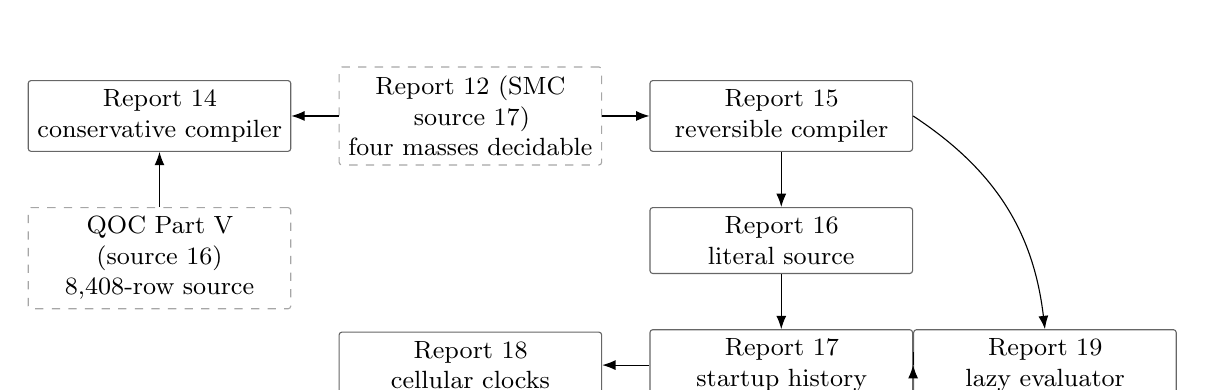
\begin{tikzpicture}[>=Latex,node distance=7mm and 6mm,
  r/.style={draw=black!60,rounded corners=1pt,align=center,font=\small,minimum height=8mm,text width=3.1cm},
  ext/.style={draw=black!35,dashed,rounded corners=1pt,align=center,font=\small,minimum height=8mm,text width=3.1cm}]
\node[ext] (r12) {Report 12 (SMC source 17)\\ four masses decidable};
\node[r,right=of r12] (r15) {Report 15\\ reversible compiler};
\node[r,left=of r12] (r14) {Report 14\\ conservative compiler};
\node[ext,below=of r14] (qoc) {QOC Part V (source 16)\\ 8,408-row source};
\node[r,below=of r15] (r16) {Report 16\\ literal source};
\node[r,below=of r16] (r17) {Report 17\\ startup history};
\node[r,left=of r17] (r18) {Report 18\\ cellular clocks};
\node[r,right=of r17,xshift=-6mm] (r19) {Report 19\\ lazy evaluator};
\draw[->] (r12)--(r15); \draw[->] (r12)--(r14); \draw[->] (qoc)--(r14);
\draw[->] (r15)--(r16); \draw[->] (r16)--(r17); \draw[->] (r17)--(r18);
\draw[->] (r17)--(r19); \draw[->] (r15.east) to[bend left=25] (r19.north);
\end{tikzpicture}
\end{center}
An arrow points from a Report to one that uses it. Report~12 supplies the matching lower bound of the threshold corollaries of Reports~14 and~15; Report~14 compiles the 8,408-row two-counter program of QOC Part~V; Report~16 instantiates the universal source that Report~15 left existential; Report~17 changes four history tags of Report~16's source; Report~18 lifts Report~17's comparison to the automaton's clock; Report~19 evaluates Report~15's automaton for Report~17's source. Report~18 also reuses Report~16's shared-offset certificate. Inside the series, Reports~20 and~26--28 (Parts~V--VI) use Reports~15, 17 and~19, and Report~28 also Report~14; SMC source~19 (Report~29) cites Report~16 for its four-versus-five boundary; GTS Part~V (Report~32) uses Report~16's loader and Turing table.

\subsection{What the Parts prove}\label{fpa:sec:overview}
\begin{itemize}
\item \textbf{Part~\ref{fpa:part:one} (Reports~15 and~14).} Every finite partial-injective guarded two-counter machine with a terminal halt compiles to a globally reversible (bijective on $\{0,1\}^{\Z}$), number-conserving binary automaton of explicit finite radius, with inputs of exactly five ones and an anchored halt word (Theorem~\ref{fpa:thm:main}); with Report~12 this makes five the exact particle threshold for globally reversible binary automata, for halt-pattern occurrence and for exact finite targets (Corollary~\ref{fpa:cor:threshold}). Report~14 proves the same number five for binary conservative automata by a different compiler for every deterministic ADD/SUB/NOP program (Theorem~\ref{fpa:bc:thm:compiler}, Corollary~\ref{fpa:bc:cor:sharp}), with a literal universal instance of radius 756,787 and a persistent halt word. Both give fixed-horizon degree-four sum-of-squares certificates with empty-or-singleton natural fibers and paid nonnegative-real variants.
\item \textbf{Part~\ref{fpa:part:two} (Report~16).} One pinned reversible two-counter machine with 122,622 controls and 141,561 literal rows is universal on a clean loader family (Theorem~\ref{fpa:ls:thm:literal}); on that family positive return and periodicity of the fixed five-particle automaton are r.e.-complete, with least period exactly $2\Theta+2$ (Corollary~\ref{fpa:ls:cor:period}).
\item \textbf{Part~\ref{fpa:part:three} (Reports~17 and~18).} Four history-tag swaps give a new source with the same semantics whose literal clock is no larger at every normalized boundary and strictly smaller at every Turing-machine cut (Theorem~\ref{fpa:st:thm:main}); first encounters determine the optimal static orientations (Theorem~\ref{fpa:st:thm:greedy}); both statements hold for the automaton's clock as well (Theorems~\ref{fpa:cc:thm:optimal} and~\ref{fpa:cc:thm:oldnew}), through the identity $\Theta=\lambda M+\mathrm{TV}(A^2)+\mathrm{TV}(B^2)+U$.
\item \textbf{Part~\ref{fpa:part:four} (Report~19).} A source-sized lazy evaluator equals the frozen ordered product of 269,291,358,255 involutions on every finite support, inverse included (Theorem~\ref{fpa:lz:thm:main}).
\end{itemize}

\subsection{Questions answered inside the series and elsewhere}\label{fpa:sec:answered}
Inside this report: Report~15's first research question (a literal universal reversible source) is answered by Part~\ref{fpa:part:two}; Report~15's limit on periodicity conclusions (the missing no-blocking premise) is supplied for Report~16's clean family by Corollary~\ref{fpa:ls:cor:period}; Report~16's first two questions (initialization cost; a lazy indexed compiler) are answered by Part~\ref{fpa:part:three} and Part~\ref{fpa:part:four}; Report~17's open old/new cellular-clock comparison is settled by Report~18, and its lazy-evaluator question by Report~19. Dated notes stand at each of these questions.

The six Reports also bear on questions of two neighbouring reports (labels of those reports are given in typewriter type):
\begin{center}
\small
\begin{tabular}{@{}p{0.43\textwidth}p{0.08\textwidth}p{0.42\textwidth}@{}}
\toprule
question & Report & effect\\
\midrule
SMC Part~IV, \S\path{smc:sl:sec:questions}, item~1: ``Print one safe universal source'' & 16 & answered in substance for Report~15's guarded syntax (122,622 controls, 141,561 rows, clean loader, all-input proofs); the lattice table of SMC Part~IV in source~13's pulse interface is still not printed\\
SMC \path{smc:tm:q:source}: a universal reversible two-counter table in the separated syntax & 16 & answered in part: a literal universal reversible two-counter table now exists, but not in source~14's separated syntax\\
SMC: ``a reversible numerical threshold, a binary upper bound'' (front matter; Part~IV item~4); source~17's non-claim ``a five-particle upper bound for binary automata''; the mass-5 cell of SMC's threshold table & 14, 15 & a binary upper bound five (Reports~14 and~15); with Report~12, five is exactly the threshold for binary and for globally reversible binary number-conserving automata (Corollaries~\ref{fpa:bc:cor:sharp} and~\ref{fpa:cor:threshold}); source~17's non-claim remains true of source~17\\
SMC \path{smc:tm:q:mass}, \path{smc:ct:q:mass}: the sharp reversible threshold & 15 & answered for automata with one unit symbol (binary); with several weight-one types three suffices (SMC Part~V)\\
QOC \path{qoc:um:thm:poly}: certificates for the 8,408-row source & 14 & bears on it: Report~14's certificate for the same source is weaker (degree four, not two) but adds the automaton's clock (note at Section~\ref{fpa:bc:sec:frontend})\\
\bottomrule
\end{tabular}
\end{center}

\subsection{Relation to the collection and to the formal project}\label{fpa:sec:relation}
\textbf{Re-proofs.} Several passages re-derive results already printed in the collection; they are kept, as second presentations, with a \wtag\ pointer naming the host statement and without any novelty claim: Report~14's Section~\ref{fpa:bc:sec:universal} (the 528- and 8,408-instruction programs and their proofs are QOC Part~V's Lemmas \path{qoc:um:lem:virtual} and \path{qoc:um:lem:prime}); the Neary--Woods table and its $(u_{10},b)$ discrepancy in Reports~14 and~16 (printed once in QOC Part~III, after Table \path{qoc:wf:tab:tm}); Report~16's front end (Section~\ref{fpa:ls:sec:frontend}); Report~15's clean-target wrapper (Section~\ref{fpa:sec:clean}), which is the forward/inverse/bridge construction of SMC source~15 (Report~10, Theorem \path{smc:ct:thm:restore}) for guarded sources, and is Bennett's uncomputation~\cite{fpa:bennett}; Report~16's history and prime-encoding invariants (Sections~\ref{fpa:ls:sec:history}--\ref{fpa:ls:sec:composition}), which make literal the existence argument of SMC Part~IV, \S\path{smc:sl:sec:safe}. Within this report the compiler clock $\tau_e(c)=3+2(Z+c)+\Delta_e-4S$ is printed in four Reports (equation~\eqref{fpa:eq:clock}, \eqref{fpa:ls:eq:caclock}, Report~17's Section~\ref{fpa:st:sec:ca}, \eqref{fpa:cc:eq:rowtime}), and Report~19 restates Report~15's ledger; the later occurrences carry pointers.

\textbf{Reviews.} At the time of this write the Hilbert's-tenth research programme (\path{Computability/HilbertTenthProblem/}) has \emph{not} reviewed Reports~14--19. Its note \path{Papers/research-wip/native-stream-queue/reviewed_report_archive_replay.md} (commit \texttt{ceb7222e9}), which restores the batch's archives from an earlier revision for replays, lists the six archives of this report as ``Relocation only'' and states that relocation is not a scientific review. Its review \path{Papers/research-wip/native-stream-queue/review_parallel_particle_reports.md} (commit \texttt{fb7e3cb47}) covers Reports~26--28 (Parts~V--VI to come), found no defect, and notes that the inherited template geometry and source simulation of Reports~15--17 remain a dependency it did not reconstruct; its review \path{review_binary_planar_four_particle31.md} (commit \texttt{16f50dcc6}) concerns Report~31 (SMC Part~VII) and separates it from the five-particle line. The programme's note \path{neary_woods_explicit_universal_tm.md} transcribes the same Neary--Woods table.

\textbf{Formal status.} No statement of this report is formalized in Lean or Rocq, and none of the Reports cites a declaration; the report's placement in the collection confers no formal status. Report~15's research question~5 and Report~16's question~4 propose mechanizing the trusted cores; Report~14's question~4 proposes formalizing its full-shift extension.

\section{Conventions and notation}\label{fpa:sec:notation}
\textbf{Labels and numbering.} Every label carries the prefix \texttt{fpa:}: Report~15's labels are \texttt{fpa:} followed by the delivered name, and the other Reports use the sub-prefixes \texttt{fpa:bc:} (14), \texttt{fpa:ls:} (16), \texttt{fpa:st:} (17), \texttt{fpa:cc:} (18) and \texttt{fpa:lz:} (19); labels added in the write are those beginning \texttt{fpa:sec:}, \texttt{fpa:part:} and \texttt{fpa:app:}, the labels \texttt{fpa:rep:}$r$\texttt{:first} and \texttt{fpa:rep:}$r$\texttt{:last} on the first and last section of Report~$r$, and \texttt{fpa:lz:sec:pinned} and \texttt{fpa:lz:sec:bytes} on two unlabelled sections of Report~19. Sections and theorems are numbered continuously through the report (Theorem $n.m$ is the $m$th numbered statement of Section~$n$). Reports~15 and~16 number their displays by hand, $(1)$, $(2)$, \dots, and their prose cites them as ``(3)'', ``(26)''; these numbers are kept as delivered and are \emph{local to the Report}: in Part~\ref{fpa:part:one} a bare $(n)$ is Report~15's display~$n$, in Part~\ref{fpa:part:two} it is Report~16's. Displays that the Reports number automatically (Reports~14, 17 and~18) are numbered $(n.m)$ by section, so they cannot be confused with the hand-numbered ones.

\textbf{Delivery paths.} The Reports name their files by their paths inside the delivered archives (for instance \code{source/source.json}, \code{reproducibility/run\_checks.py}, \code{companions/report15/}, \dots). Those names are kept in the text. The \texttt{README.md} of this report maps every delivery path to its shipped name (shipped files carry the prefixes \path{14-five-binary-}, \path{15-rev-five-}, \path{16-literal-source-}, \path{17-startup-}, \path{18-cell-clock-} and \path{19-lazy-eval-}), and lists the files that are not shipped: byte copies of other files, the delivered PDFs and checksum ledgers, the companion copies of Reports~12 and~15, and eighteen heavy generated files (among them both \code{source.json} tables, each 32,034,272 bytes) that the shipped programs rebuild in seconds (README, ``Reconstructing the excluded data'').

\textbf{Notation.} No symbol of a Report was renamed: each Part uses its Report's symbols. The same letter often means different things in different Reports; the table lists the collisions. In the text written for the merge, these notions are named in words.
\begin{center}
\small
\begin{longtable}{@{}p{0.08\textwidth}p{0.42\textwidth}p{0.42\textwidth}@{}}
\toprule
symbol & Reports~15--19 (Parts~\ref{fpa:part:one}--\ref{fpa:part:four}) & Report~14 (second half of Part~\ref{fpa:part:one}) and others\\
\midrule
\endhead
$m$ & number of source controls & same (all controls, halt included)\\
$p$ & number of nonzero-update branches & number of ADD or SUB \emph{rows} (a SUB row has two branches)\\
$a$ & number of zero-update branches & a counter value ($c_0=a$, $c_1=b$; initial $a_0,b_0$)\\
$n$, $z$ & Report~19: $n$ is the mass of a support & $n$ NOP rows, $z$ SUB rows\\
$D$ & $2m+4p$, the gap alphabet of signed modes & $m+2p$, the gap alphabet of unsigned codes\\
$S$ & $2D+2$, the home offset of the close pair & ---\\
$Z$ & $10B_3+10+2J=40D+60+2J$, the counter buffer & $4K=16D+20$\\
$K$ & Report~16: the source horizon in primitive rows of the certificates ($141{,}565K$ witnesses) & $4D+5$, the component and contact distance\\
$L$, $R$ & Report~15: travel constant $L=3D+4$ and radius bound $R$, eq.~(18); Reports~16--18: half-tape integers $L,R$ & radius $R=30D+37$; $L,R$ also half tapes in Section~\ref{fpa:bc:sec:universal}\\
$T$ & Report~15: context radius of a gate, and a microedge count in Proposition~\ref{fpa:prop:cycle}; Reports~16--18: the scratch counter & scratch register; tick and clock variable in the certificates\\
$H$, $h$ & Report~15: source horizon $H$ of a certificate and halt control $h$; Reports~16--18: history counter $H$; $\mathsf H$ a home mode & horizon $h$ of a certificate; $H$ the terminal residual\\
$\Theta$ & the automaton's clock: microedges to the first plus-halt home & ---\\
$\lambda$ & Report~18: $3+2Z-4S=36{,}684{,}691$ for the universal source & ---\\
$J$ & the class cutoff of guards & a Turing state ($J1=(u_{10},b)$ is the halt cell), as also in Report~16's Table~16\\
$A$, $B$ & Reports~16--18: the two physical counters; Report~15: $A_t$ a residual, $B$ a swap radius or normalized-branch count & $B$ the number of branches\\
$F$ & Report~15: one automaton step $P\circ E$; Report~19: the number of factors & ---\\
$M$, $U$ & Report~18: moving-row and zero-update counts; Report~15 certificates: $M$ bounds the initial counters & $U_t$ the one-hot residual\\
\bottomrule
\end{longtable}
\end{center}
Tempting false readings: Report~14's $D=m+2p$ is not Report~15's $D=2m+4p$ (they count different alphabets, and $p$ is not the same count); the two radius bounds $30D+37$ (Report~14) and eq.~(18) (Report~15, quadratic in $D$) bound different automata; Report~16's $K$ is a horizon, not Report~14's contact distance; $J$ in ``$J1$'' is a Turing state, not a class cutoff.

\section{Status and non-claims}\label{fpa:sec:nonclaims}
The six Reports are AI-assisted research manuscripts; Report~14's delivery README says ``prepared with AI assistance''. They are unrefereed, not formalized, and not yet reviewed by the research programme (Section~\ref{fpa:sec:relation}). Each Report states its own limits; all of them are kept in its text, and they are collected here.
\begin{itemize}
\item \textbf{Report~15.} Mathematical proofs with independent computational and mathematical audits, not proof-assistant formalizations or claims of novelty or priority. Universality is in an effective finite-input halting-observation sense; there is no claim of intrinsic universality, real-time simulation, efficient input conversion, radius optimality, or a printed universal binary truth table. The universal source of Corollary~\ref{fpa:cor:universal} is existential in Report~15 (Part~\ref{fpa:part:two} materializes one); the executable example is finite and accepting, not universal. The radius bound is an upper bound, and writing the truth table would be impractical. The certificate horizon is a compiler argument; no unbounded single-fold representation follows; the paid variant concerns the nonnegative orthant with natural initial counters, not unrestricted reals. Periodicity and positive return need an extra no-blocking premise for general sources. The threshold depends on Report~12's separate proof. The Alhazov--Imai construction was not inspected in full; an incomplete search is not a novelty argument; no first-construction claim is made.
\item \textbf{Report~14.} No reversibility, intrinsic universality, efficient input preparation, efficient CA time or minimal radius is claimed. The universal truth table ($2^{1,513,575}$ rows) and the 1,272,679,260 indexed cases are specified, not materialized; universality rests on the Neary--Woods source and all-input proofs, not on table size. The horizon is fixed at emission; there is no unbounded single-fold representation and no universal-polynomial record; the $h=1$ universal schema is not an accepting universal computation. The sharp threshold depends on Report~12, excludes infinite backgrounds, active zero-weight states, several unit labels, signed weights and nonuniform rules, and is not a priority claim; the literature search was limited. The loader is not a polynomial-time map in the length of the Turing-machine input. Finite tests do not replace the proofs.
\item \textbf{Report~16.} An ordinary mathematical proof with executable audits, not a proof-assistant formalization, efficient simulation, novelty claim or size record. The automaton's factor list, truth table and universal-instance quartic are not materialized. Empty-tape initialization has a predicted clock near $8\cdot10^{13}$ source steps; only small literal macros and the fresh entry were executed. Universality and no-blocking hold under the clean-input promise; the clean wrapper and its automaton are theorem-level only; the four-mass lower bound is imported.
\item \textbf{Report~17.} No raw cellular-automaton speed comparison and no completion of a universal program is claimed (Report~18 adds the clock comparison); the old 79,936,151,060,302-step startup is derived, not executed; an equal-history internal state can be slower (28 versus 104 steps). Optimality is within the fixed templates. Report~16's machine and artifacts are not revised; equal counts do not identify the two automata. Not a formalization, novelty, efficiency or size claim.
\item \textbf{Report~18.} The comparison holds within the fixed static-orientation, recorder, prime-template and compiler class. No novelty, optimal universal-machine size, unrestricted speedup or host-runtime claim; no uniform ratio of arrival times, no equal-time alignment; no automaton orbit or giant rule array was executed; symbolic factor and radius counts are not allocated objects.
\item \textbf{Report~19.} An implementation-equivalence result, not a new universality proof, a proof-assistant formalization or a novelty claim. No constant-time or polylogarithmic cost guarantee; the 128 universal microsteps do not complete startup or a Turing transition; no eager universal comparison was made; the benchmark's resource figures are environment-specific.
\end{itemize}

\fpapart{Five particles suffice in binary automata (Reports 15 and 14)}{fpa:part:one}

\reportopening{15}{Globally reversible binary computation with five particles}{An explicit finite-radius compiler and counted finite-horizon Diophantine certificates}{Report 15 \quad Mathematical construction and reproducible audit}

\begin{reportabstract}{15}
A finite partial-injective deterministic machine with two natural counters is
compiled into one time-independent cellular automaton on the full binary shift.
Every encoded configuration has exactly five occupied sites and an otherwise
zero background. The automaton is globally reversible, conserves the ordinary
number of ones, and has an explicit finite radius. Full-shift reversibility is
proved by an isolated equal-mass pattern-swap lemma valid on arbitrary dense or
infinite inputs; simulation correctness is a separate matching argument on a
precisely delimited admissible set. Forward and backward copies of a subdivided
counter computation reflect at missing edges. The classical existence of a
universal reversible two-counter source gives a five-particle universality
existence theorem, without pretending that a literal universal source table has
been materialized here. We count all gate factors and radii, give exact clocks,
and construct degree-at-most-four sum-of-squares certificates for fixed finite
source horizons, with exact natural witness fibers and explicit costs. A small
fully materialized accepting machine, its complete raw particle orbit, vector
figure, and exact replay tests accompany the proof. A separate, byte-preserved
four-mass decidability report supplies the matching lower bound. These are
mathematical proofs with independent computational and mathematical audits,
not proof-assistant formalizations or claims of novelty or priority.
\end{reportabstract}

\wtag\ Delivered as \path{Reversible_Binary_Five_Particle_Package.zip} (batch~82, archive~15; arrival \texttt{db37d18c8}), dated 3~October 2026; files placed by \texttt{bca6383e9} with the prefix given in Appendix~\ref{fpa:app:provenance}. This Report is the base of the merge: its text is printed in full, with its three \verb|\input| files inlined.

\section{Scope and theorem}\label{fpa:rep:15:first}
We use $\N=\{0,1,2,\ldots\}$. A binary configuration is an element
$x\in\{0,1\}^{\Z}$. Its support is $\supp(x)=\{i:x_i=1\}$; for finite support,
its numerical mass is $M(x)=|\supp(x)|$. A radius-$R$ cellular automaton (CA) is
given by one map $f:\{0,1\}^{2R+1}\to\{0,1\}$ used at every integer site and
every time. Reversible means bijective on the \emph{entire} full shift, not
merely injective on encoded or finite configurations. We call it
number-conserving when $M(Fx)=M(x)$ for every finite-support $x$. The all-zero
configuration is fixed by the construction.

\begin{theorem}[Effective reversible five-particle compiler]\label{fpa:thm:main}
Let $C$ be a finite deterministic partial-injective two-natural-counter machine
of the form in Section~\ref{fpa:sec:source}, with $m$ controls, $p$ nonzero-update
branches, $a$ zero-update branches and class cutoff $J$. Suppose its designated
halt control has no outgoing branch. An effective procedure constructs:
\begin{enumerate}
\item a binary, translation-equivariant, time-independent, finite-radius CA
$F$ that is bijective on $\{0,1\}^{\Z}$ and preserves finite numerical mass;
\item a computable injection from source IDs into configurations with exactly
five ones and zero elsewhere; and
\item one finite anchored binary word whose occurrence along the encoded
forward orbit is equivalent to eventual reachability of the source halt
control.
\end{enumerate}
The factor count, radius bound, encoding diameter and exact source-edge clock
are given explicitly below. No spatial checkerboard, external step counter,
changing background or additional stored particle is used.
\end{theorem}

\begin{corollary}[Universality by a fixed source]\label{fpa:cor:universal}
There exists a fixed globally reversible, number-conserving binary CA of finite
radius for which occurrence of a fixed finite anchored halt word is undecidable
on a computable family of initial configurations containing exactly five ones.
\end{corollary}
\begin{proof}
Choose a fixed universal deterministic Turing machine, apply the effective
reversible two-counter simulation theorem of Morita~\cite{fpa:morita1996}, make the
terminal-control normalization in Section~\ref{fpa:sec:source}, then apply
Theorem~\ref{fpa:thm:main}. The resulting source, compiler parameters, CA and observer
are fixed; only the effectively encoded finite input varies.
\end{proof}

This is universality in an effective finite-input halting-observation sense.
It is not a claim of intrinsic universality, real-time simulation, efficient
input conversion, radius optimality, or a printed universal binary truth table.
The explicit executable example in this release is finite and accepting, but
is \emph{not} universal. The universal reversible source is supplied by an
existence-by-effective-construction theorem, rather than by an instantiated
list of universal transition rows in this report.

\wtag\ The literal universal reversible source that this paragraph says is absent is supplied in Part~\ref{fpa:part:two}: Report~16 instantiates it (Theorem~\ref{fpa:ls:thm:literal}) and feeds it to the compiler of Theorem~\ref{fpa:thm:main}, so the fixed automaton of Corollary~\ref{fpa:cor:universal} now has explicit parameters (Section~\ref{fpa:ls:sec:binary}).

\section{Source machine and primary attribution}\label{fpa:sec:source}
A source ID is $(q,c_0,c_1)\in Q\times\N^2$. Each branch $e$ specifies source
$q_e$, target $q'_e$, a selected counter $j_e\in\{0,1\}$, an update
$\Delta_e\in\{-1,0,1\}$ and a finite Boolean predicate $G_e(c_0,c_1)$ built
from atoms $c_j=k$ and $c_j>k$, where $k\in\N$. The other counter is unchanged.
The following are hypotheses on \emph{all} source IDs:
\begin{enumerate}
\item enabled branches have natural-number outputs;
\item branch domains with a common source control are pairwise disjoint;
\item actual branch image domains with a common target control are pairwise
disjoint.
\end{enumerate}
The exact image predicate is
\[
 I_e(c')=\bigl[c'-\Delta_e\mathbf e_{j_e}\in\N^2\bigr]
 \wedge G_e(c'-\Delta_e\mathbf e_{j_e}).                 \tag{1}\label{fpa:eq:image}
\]
It is computed from the branch; it is not an independently trusted guard.
These hypotheses make the source transition relation a partial injection.
An ID outside every branch domain is stuck. It counts as a halt observation
only if its control is the designated $h$.

Choose a finite $J$ such that every domain and image predicate is determined
by each counter's class
\[
 \mathcal K_J=\{0,1,\ldots,J,\star\},\qquad \star=\{J+1,J+2,\ldots\}.
\]
Finite class enumeration verifies disjointness for predicates satisfying this
cutoff promise. The parser uses a sufficient syntactic criterion that includes
all atom thresholds and their updated-counter shifts. This criterion can
reject logically redundant formulas even if a smaller cutoff would suffice;
that is a deliberate validation restriction. Counter values are exact
nonnegative integers. Floats and Boolean values masquerading as integers do
not provide source IDs.

\subsection{What is imported from Morita, and what is added here}
Morita's 1996 Definitions 2.1--2.3 (printed pp.~304--306) specify natural-counter
IDs and reversible counter-machine transitions. Theorem 4.1 (p.~313) reduces
reversible $k$-counter computation to two counters by an effective prime
encoding. Theorem 4.2 (p.~319) simulates each deterministic Turing machine by a
reversible two-counter machine~\cite{fpa:morita1996}. Thus no uncounted history or
work register remains beyond the final two counters and finite control.

Its row types translate into this interface as follows:
\begin{center}
\begin{tabular}{lll}\toprule
Row type & Domain on selected counter $c$ & Update\\\midrule
zero test & $c=0$ & $0$\\
positive test & $c>0$ & $0$\\
increment & true & $+1$\\
decrement & $c>0$ & $-1$\\
no change & true & $0$\\\bottomrule
\end{tabular}
\end{center}
Here $J=1$ suffices for all domains and exact images. For example, increment's
image is positive, while an increment restricted to zero has image exactly
one. A reverse gate must use these images, not blindly reuse a forward test.

The cited definition designates a final control but does not explicitly ban
outgoing rows from it. \emph{Our normalization} deletes all such rows. This
restricts a partial injection and preserves first reachability of that control.
It does not claim to preserve post-halt behavior. If a predecessor-free initial
control is wanted, Morita--Imai 2001, Lemma 3.5 (printed pp.~245--246), supplies
a reversible two-counter normal form with no row entering its initial
control~\cite{fpa:moritaimai2001}. Apply that first, then delete final-control exits.
This extra condition is used for exact finite reflection cycles and the clean
target construction, but not for the forward halt-pattern equivalence.

Prime encoding can be expensive in time and value. The input conversion need
only be computable. No numerical values of $m,p,a$ for a literal universal
reversible table are claimed here, and no nonreversible source table from a
previous report is silently substituted.

\wtag\ Report~16 (Part~\ref{fpa:part:two}) gives such numerical values for one literal universal reversible table in this schema: $m=122{,}622$ controls, $141{,}561$ branches and $J=0$. The nonreversible 8,408-row source of the second half of this Part (Report~14) is not that table, and Report~16 does not use it.

\section{An isolated swap on every binary input}\label{fpa:sec:swap}
The all-input lemma is the reason malformed configurations cannot undermine
global reversibility.

Fix $B\ge1$ and two finite supports $P,Q\subseteq[-B,B]$ with equal nonzero
cardinality $k$. Suppose $P$ and $Q$ are not translates. Their coordinate zero
is an assigned key, not necessarily the leftmost occupied site. A position $u$
is a \emph{raw key} in $x$ when the ones in $[u-B,u+B]$ are exactly $u+P$ or
exactly $u+Q$. Let a local, translation-covariant contextual predicate read
within radius $T$ of the key, and assume it has the \emph{same truth value at
paired endpoints} when outside bits are fixed. Set
\[
 L_B=3B+1,\qquad M_B=\max(L_B+B,T+B)+1,\qquad r_B=M_B+2B. \tag{2}\label{fpa:eq:swapconst}
\]
A raw key $u$ is eligible if:
\begin{enumerate}
\item its only ones in $[u-L_B,u+L_B]$ are its displayed $k$ particles;
\item no other raw key lies at distance at most $M_B$; and
\item the contextual predicate holds.
\end{enumerate}
Swap $u+P$ and $u+Q$ at all eligible keys simultaneously and leave every other
bit unchanged. Denote this map by $\Swap(P,Q;B,G,T)$.

\begin{lemma}[All-input isolated-swap lemma]\label{fpa:lem:swap}
The displayed map is an involutive binary CA of radius at most $r_B$. It
preserves numerical mass on every finite configuration. These statements hold
without any density, finite-support or well-formedness promise on the input
for the involution and locality claims.
\end{lemma}
\begin{proof}
Distinct eligible keys are farther than $M_B$ apart. Their radius-$B$ cores
are disjoint. This makes even an infinite family of simultaneous rewrites
well-defined. No other active core intersects the radius-$L_B$ isolation halo
or radius-$T$ contextual window of an active key, since intersection would
force key distance at most $L_B+B$ or $T+B$.

Write $y$ for the rewritten configuration. We first prove that the \emph{entire
raw-key set}, not merely the active subset, is unchanged. A raw-test window
that changes intersects the rewritten core of some active key $u$. Its key
$v$ has $|v-u|\le2B$, so its entire window is contained in
$[u-3B,u+3B]$. In $x$ this larger interval has just $u+P$ or $u+Q$ as its $k$
ones. In $y$ it has precisely the other support. If the window at $v$ is raw
at either endpoint, its $k$ ones must therefore be the \emph{entire} support
of the active pattern at that endpoint. Nontranslation of $P,Q$ forces its
label to be that of the active pattern. A nonempty finite set cannot equal a
nonzero translate of itself, so $v=u$. Every active key remains raw after
its own rewrite. All other raw-test windows that could change are nonraw on
both sides. This proves raw-key invariance, including changes involving a
required zero in a matching window.

Consequently, the no-other-raw-key condition is invariant. An active key
retains isolation because its only changed particles are its own equal-mass
core. It retains the contextual condition by the paired-endpoint assumption
and separation from all other active cores. An inactive raw key that is
blocked by another raw key stays blocked. An inactive raw key with no such
blocker is farther than $M_B$ from every active key, so none of its code,
isolation or context tests can change. Thus eligibility is unchanged at every
key. A second application rewrites exactly the same disjoint cores and
restores their original patterns: $\Swap^2(x)=x$ for every $x$.

For an output site $i$, only keys within $B$ can write at $i$. A key's
eligibility is determined by its radius-$(M_B+B)$ input window, which covers
the raw-key exclusion, isolation and context tests. Radius $M_B+2B$ about $i$
therefore suffices. Every test is in relative coordinates, proving translation
equivariance. Finally, for finite input there are finitely many disjoint active
cores, and each replaces $k$ ones by $k$ ones. This proves mass conservation.
\end{proof}

The guard requirement is genuinely cross-endpoint. Giving the $P$ endpoint
a constant true guard and the $Q$ endpoint a constant false guard would break
the involution, although each constant is individually insensitive to bits.
Every contextual gate below uses one identical predicate of unchanged exterior
bits at both endpoints, so it meets the stronger requirement directly.

A finite ordered composition of these gates is a full-shift reversible,
number-conserving CA. Its inverse applies the same involutions in reverse
order. The ordered product itself need not be an involution.

\section{Five-particle geometry}\label{fpa:sec:geometry}
There are $m+2p$ unsigned head modes: $\Hh_q$ for each source control, and
$\Oo_e,\Ii_e$ for each nonzero branch. Give each signed mode $u^+,u^-$ a
\emph{distinct} gap $d(u^\pm)$ in $\{1,\ldots,D\}$, where
\begin{align}
 D&=2m+4p, & S&=2D+2, & B_2&=D+1,\notag\\
 L&=3D+4, & B_3&=4D+5, & Z&=10B_3+10+2J=40D+60+2J. \tag{3}\label{fpa:eq:constants}
\end{align}
A signed head $u^\sigma$ at anchor $x$ is the pair $\{x,x+d(u^\sigma)\}$.
The anchor is always its leftmost particle, even during leftward travel.

The home encoding, with origin zero, is
\[
 \enc(q,c_0,c_1)=
 \{-(Z+c_0),\;0,\;Z+c_1,\;S,\;S+d(\Hh_q^+)\}.        \tag{4}\label{fpa:eq:encoding}
\]
It has exactly five distinct occupied sites. Three singleton markers encode
the left endpoint, origin, and right endpoint. The endpoints carry counter
values by their distances to the origin. The remaining close pair encodes all
control and sign information. The singleton particles have no hidden colors.
The initial diameter is $2Z+c_0+c_1$.

On the admissible microstates below, marker separations are at least $Z$.
All head-to-marker distances are at least $S-D=D+2$, while the head's internal
gap is at most $D$. Thus the head is the unique close pair. Removing it leaves
three markers whose middle member is the origin. This proves effective
geometric decoding and disambiguates roles with only binary sites. In
particular, signed mode information is paid for in pair spacing and radius,
not in additional particles or a larger alphabet.

\section{The partial micrograph and its exact clock}\label{fpa:sec:micrograph}
For a nonzero branch $e$, write $v=-1$ for the left counter and $v=+1$ for the
right. Let $o$ be the origin, $m$ the selected endpoint, and $c$ its old counter
value. Replace its source edge by the following finite path of unsigned
microstates:
\begin{enumerate}
\item \textbf{Dispatch.} Replace a home $\Hh_{q_e}$ head at $o+S$ by an
$\Oo_e$ head at $o+vS$, under $G_e$.
\item \textbf{Outbound travel.} Move its anchor by $v$ at each microedge,
from $o+vS$ to $m-vS$.
\item \textbf{Endpoint interaction.} Move the selected endpoint to
$m'=m+v\Delta_e$ and change the head to $\Ii_e$ at $m'-vS$.
\item \textbf{Return travel.} Move its anchor by $-v$ at each microedge until
$o+vS$.
\item \textbf{Commit.} Change to $\Hh_{q'_e}$ at $o+S$, under the exact
image predicate $I_e$ evaluated on the post-counters.
\end{enumerate}
A zero-update branch is one directly guarded home-to-home microedge.

\begin{definition}[Admissible microstates]\label{fpa:def:admissible}
The unsigned admissible set consists of every home ID in $Q\times\N^2$ and
only the strict intermediate configurations on a displayed subdivision of an
\emph{enabled} source edge $e,c$ satisfying $G_e(c)$. The doubled admissible
set contains a plus and minus copy of exactly this set.
\end{definition}

Arbitrary geometrically plausible outbound or return packets are \emph{not}
included merely because their spacings look reasonable. Branch-domain and
exact-image compatibility are part of admissibility. Global CA reversibility
will not depend on this restriction, but simulation closure does.

\begin{lemma}[Injective subdivision and time]\label{fpa:lem:subdivision}
The micrograph on admissible unsigned states is a partial injection. A
nonzero branch at selected counter $c$ has exactly
\[
 \tau_e(c)=3+2(Z+c)+\Delta_e-4S                         \tag{5}\label{fpa:eq:clock}
\]
microedges; a zero-update branch has one.
\end{lemma}
\begin{proof}
Distinct branch labels distinguish intermediate paths. An outbound mode
retains old counters and branch label; a return mode retains the post-counters
and branch label, from which the old counters are recovered. Its anchor fixes
its unique position within that corridor. Home successors are unique by
source-domain disjointness. Home predecessors are unique by disjointness of
actual branch images. Therefore subdivisions neither branch nor merge
improperly. Their outbound and return travel lengths are respectively
$Z+c-2S$ and $Z+c+\Delta_e-2S$. Both are nonnegative with a large strict margin
by (3). Adding dispatch, endpoint interaction and commit gives (5).
\end{proof}

For motion of direction $w\in\{-1,+1\}$ near a marker $m$, a marker behind
the head has anchor $x=m+wt$, with travel allowed for $t\ge S$. A marker ahead
has $x=m-wt$, with travel allowed for $t>S$; at $t=S$ the next edge is the
appropriate interaction. There is no travel edge from behind distance $S-1$
into a dispatched or reversed state. These endpoint conventions are essential
to the matching argument.

\section{The edge matching as concrete pattern swaps}\label{fpa:sec:edge}
For each unsigned microedge $z\to z'$, we want the transposition
$z^+\leftrightarrow z'^-$. The following finite list of individual isolated
swaps is composed once, in any one fixed order, to form the edge block $E$.
The fixed order is part of the compiled local rule.

\subsection{Free flight}
For each moving mode $u$ with direction $w$, use a two-particle gate with
$B=B_2$, $T=0$ and supports
\[
 P=\{0,d(u^+)\},\qquad Q=\{w,w+d(u^-)\}.              \tag{6}\label{fpa:eq:free}
\]
Its invariant key is the \emph{predecessor} anchor $x$. It is eligible on an
admissible predecessor exactly when no marker lies within $[x-L,x+L]$.
The gate's raw key is unique because any raw pair must be the unique close
pair. The reverse endpoint still checks isolation at $x$, not at its new
anchor $x+w$.

\subsection{Contact travel}
For each moving $u$ of direction $w$, use three-particle gates keyed at the
contacted marker zero, with $B=B_3,T=0$:
\begin{align}
 \{0,wt,wt+d(u^+)\}&\longleftrightarrow
 \{0,w(t+1),w(t+1)+d(u^-)\}, && S\le t\le L; \tag{7}\label{fpa:eq:behind}\\
 \{0,-wt,-wt+d(u^+)\}&\longleftrightarrow
 \{0,-w(t-1),-w(t-1)+d(u^-)\}, && S+1\le t\le L. \tag{8}\label{fpa:eq:ahead}
\end{align}
These cover the complement of free flight on valid predecessors near a marker.
All integer $t$ in the displayed ranges give separate finite gate factors.

\paragraph{The free/contact boundary, both directions.}
Behind a marker, departure from predecessor distance $L$ uses (7), ending
at distance $L+1$. The potential inverse of (6) still tests the predecessor
key at distance $L$, and therefore sees the marker and is blocked. Ahead of
a marker, arrival from predecessor distance $L+1$ uses (6), ending at distance
$L$. There is no gate (8) with predecessor distance $L+1$, so it cannot compete.
At behind distance $S$, an outgoing travel edge exists but no incoming travel
edge from $S-1$ does; dispatch or endpoint reversal supplies that incoming
edge. At ahead distance $S$, travel has no outgoing edge; endpoint interaction
or commit supplies it. These statements remain true for $w=-1$ because (6)
preserves the predecessor key rather than redefining it by the sign of travel.

\subsection{Dispatch, endpoint and commit}
Each nonzero branch supplies three triple gates, with $B=B_3$:
\begin{align}
 \{0,S,S+d(\Hh_{q_e}^+)\}
 &\longleftrightarrow\{0,vS,vS+d(\Oo_e^-)\},          \tag{9}\label{fpa:eq:dispatch}\\
 \{0,-vS,-vS+d(\Oo_e^+)\}
 &\longleftrightarrow\{v\Delta_e,v\Delta_e-vS,
 v\Delta_e-vS+d(\Ii_e^-)\},                           \tag{10}\label{fpa:eq:endpoint}\\
 \{0,vS,vS+d(\Ii_e^+)\}
 &\longleftrightarrow\{0,S,S+d(\Hh_{q'_e}^-)\}.       \tag{11}\label{fpa:eq:commit}
\end{align}
The dispatch gate uses $G_e$, the commit gate uses $I_e$, and the endpoint gate
has no context. The endpoint gate's invariant key is the \emph{old} endpoint
coordinate, including when its reverse endpoint is inspected.

For a zero-update branch use the triple gate
\[
 \{0,S,S+d(\Hh_{q_e}^+)\}\longleftrightarrow
 \{0,S,S+d(\Hh_{q'_e}^-)\},                           \tag{12}\label{fpa:eq:zero}
\]
with the same source/image predicate $G_e=I_e$.

\subsection{Reading bounded counter classes without storing anything}
At a home gate's origin key, read the bits at $-(Z+k)$ and $Z+k$ for
$0\le k\le J$. In an admissible state one present bit determines its finite
class; all-zero reads indicate $\star$. If more than one bit appears on a
side on a malformed input, define the guard false. This is a finite Boolean
word test of radius $T=Z+J$.

All read positions are outside the swapped support. At each of (9), (11)
and (12), the same origin key, same exterior bits, and same predicate are used
at both endpoints. Hence the contextual gate satisfies Lemma~\ref{fpa:lem:swap}
on the full shift, not just the intended data.

Every displayed triple has three distinct sites, one uniquely close pair of
gap at most $D$, and other gaps greater than $D$. Plus and minus gaps differ,
so the two supports are not translates. Their extremes lie in $[-B_3,B_3]$;
in particular, the largest contact departure endpoint is $L+1+D=B_3$.
Other markers are outside its particle-isolation halo because
$Z>3B_3+1$, with margin even for the old-key displacement in (10). Any raw
triple must contain the unique close pair and its nearby marker. Its gap
identifies the endpoint label, and then its anchor identifies the key. Thus
there is only one raw key on an admissible state. A large contextual
raw-key-exclusion radius cannot accidentally veto the intended gate.

\begin{lemma}[Matching and closure]\label{fpa:lem:matching}
On the doubled admissible set, $E$ acts exactly as the matching that exchanges
$z^+$ with $z'^-$ for each unsigned microedge $z\to z'$, and fixes unmatched
vertices. No order choice among its fixed gate factors changes this action.
\end{lemma}
\begin{proof}
A plus state belongs only to its outgoing microedge; a minus state belongs only
to its incoming microedge. Equations (6)--(12) realize precisely those edges,
with the travel-boundary cases above eliminating overlap and gaps. At homes,
plus incidence is unique by domain disjointness and minus incidence by exact
image disjointness. Conversely, a minus home passing $I_e$ has a unique natural
predecessor $c=c'-\Delta_e\mathbf e_{j_e}$ satisfying $G_e(c)$ by (1).
Its inverse commit or direct gate therefore enters an \emph{included}
subdivision, not spurious moving geometry. Forward dispatch similarly enters
an enabled subdivision. Branch labels preserve intermediate uniqueness.
Thus every gate stays in the admissible set and realizes its one matching
edge there. Once one factor moves a vertex to its partner, no other matching
edge is incident at the partner, so subsequent factors do nothing to it.
\end{proof}

The matching claim is restricted to admissible configurations. It is not a
claim that $E$ itself is an involution on every malformed configuration.
Full-shift reversibility follows instead from the independently involutive
factors, which require no matching hypothesis.

\section{Phase flip, reflection and observation}\label{fpa:sec:reflection}
The signed phase block $P$ uses the following factors. For each moving $u$,
include the pair gate
\[
 \{0,d(u^+)\}\longleftrightarrow\{0,d(u^-)\}
 \quad(B_2,T=0).                                    \tag{13}
\]
For each moving $u$, each $s\in\{-1,+1\}$ and $S\le t\le L$, include
\[
 \{0,st,st+d(u^+)\}\longleftrightarrow
 \{0,st,st+d(u^-)\}\quad(B_3,T=0).                   \tag{14}
\]
For each $q\in Q$, include the home triple
\[
 \{0,S,S+d(\Hh_q^+)\}\longleftrightarrow
 \{0,S,S+d(\Hh_q^-)\}\quad(B_3,T=0).                 \tag{15}
\]
On an admissible state, precisely one phase gate is active. At a moving anchor
with no marker within $L$, it is the pair gate. Otherwise there is one nearby
marker at a distance in $[S,L]$, and exactly one contact phase gate applies.
At a home the origin supplies its home phase gate. A phase flip keeps the
anchor fixed, so it cannot change this classification. The fixed-order block
$P$ therefore acts as sign reversal on admissible states.

Define \emph{one CA time step} to be
\[
                         F=P\circ E.                \tag{16}\label{fpa:eq:F}
\]
This is one fixed composition of finitely many translation-equivariant local
rules. Composition of radius-$r_i$ rules has radius at most $\sum_i r_i$.
Evaluating the factors internally is an algorithm for the single local map
$f$; it is not an externally alternating CA, a spatial phase convention or an
extra clock layer. Its full-shift inverse is the reverse list of the same
involutions. Thus Lemma~\ref{fpa:lem:swap} proves full-shift bijectivity and finite
mass conservation independently of simulation validity.

On an admissible plus vertex with successor, $E$ moves to its successor's
minus copy and $P$ restores plus. On a minus vertex with predecessor, $E$
moves to its predecessor's plus copy and $P$ restores minus. At a missing
outgoing or incoming edge, $E$ fixes the vertex and $P$ flips its sign in one
step. This proves the desired reversible reflection dynamics.

\begin{proposition}[Exact reflection cycle]\label{fpa:prop:cycle}
If a starting source ID has no predecessor and its forward computation reaches
terminal halt after $T$ microedges, the encoded orbit has exactly $2T+2$
states, visiting the full forward history, then the full reverse history, then
returning to its initial plus state.
\end{proposition}
\begin{proof}
A finite partial-injective path from a predecessor-free start to a terminal
vertex has $T+1$ distinct unsigned vertices. Plus and minus copies are distinct
because their gaps differ. The forward and backward traversals take $T$ steps
each; the two boundary sign flips each take one. This visits each of the
$2T+2$ signed vertices once before returning.
\end{proof}

In particular, a reversible orbit does not enter a separate periodic attractor
or freeze at halt. Its backward history is part of its own cycle.

The observer is the anchored binary word on $[0,S+D]$ with ones exactly at
\[
                 \{0,S,S+d(\Hh_h^+)\},              \tag{17}\label{fpa:eq:observer}
\]
and zeros at all other sites in that interval. Its length is $3D+3$. Both
endpoints lie outside the word. The unique head gap identifies the halt plus
home. No moving head or other home mode can give that gap. The interval's
origin and fixed head position force the home geometry on admissible states.

If the forward source run reaches $h$, the observer occurs. For the converse,
a different stuck home may reflect, but a backward traversal cannot newly
reach an $h$ home: that would require an outgoing microedge from $h$, and
$h$ is terminal. Reflection only retraces the same path component. Therefore
the observer occurs along the full encoded orbit if and only if the forward
source computation reaches $h$. The negative halt code is different. This
also explains why terminal-control normalization is required for the stated
unrestricted-in-time observation equivalence.

\section{The exact resource ledger}\label{fpa:sec:ledger}
All factors use alphabet $\{0,1\}$; all encoded microstates have mass five.
Unoccupied guard-reading positions store no data. With constants (3), the
factor counts and individual radius bounds are:
\begin{center}
\begin{tabular}{lrr}\toprule
Factor category & Number & Radius bound\\\midrule
Pair gates & $4p$ & $r_2=6D+8$\\
Unguarded triple gates & $8pD+23p+m$ & $r_3=24D+32$\\
Contextual triple gates & $2p+a$ & $r_c=Z+J+12D+16$\\\midrule
All factors & $8pD+29p+m+a$ & sum below\\\bottomrule
\end{tabular}
\end{center}
To check the count, each of $2p$ moving modes has one free-flight and one
pair-phase gate. Its contact travel contributes $(L-S+1)+(L-S)=2D+5$
triples; contact phase contributes $2(L-S+1)=2D+6$. Add $p$ unguarded endpoint
triples, $m$ home-phase triples, $2p$ contextual dispatch/commit triples, and
$a$ contextual direct triples. This gives every row above.

For $T=0$, (2) gives radius $6B+2$, which yields $r_2,r_3$ after substitution.
For contextual triples, $T=Z+J$ dominates and the radius is
$T+3B_3+1=r_c$. Therefore a valid explicit composition radius is
\begin{align}
 R={}&4p(6D+8)+(8pD+23p+m)(24D+32)\notag\\
     &+(2p+a)(Z+J+12D+16).                            \tag{18}\label{fpa:eq:radius}
\end{align}
This is a counted upper bound, not a minimum radius. A literal local truth
table has $2^{2R+1}$ binary entries. It can be generated by finite composition
of the factor algorithms, but writing it explicitly would typically be far
larger than the gate description. Compilation is effective without any claim
that this truth-table expansion is practical.

For a source path of $H$ branches with old selected values $c_{t,j_t}$, its
first halt time is
\[
 T=\sum_{t=0}^{H-1}\left\{
 \begin{array}{ll}1,&\Delta_{e_t}=0,\\
 3+2Z+\Delta_{e_t}-4S+2c_{t,j_t},&\Delta_{e_t}\ne0.
 \end{array}\right.                                 \tag{19}\label{fpa:eq:totalclock}
\]
A certificate's source horizon is $H$, not this counter-dependent CA time.
After at most $H$ source steps, both counters are at most their initial value
plus $H$, their sum is at most the initial sum plus $H$, and the entire
subdivided path remains inside a span of at most
\[
                         2Z+c_{0,0}+c_{0,1}+H.       \tag{20}\label{fpa:eq:diameter}
\]
The head stays between endpoints throughout. These are value/diameter bounds;
they are not bit-complexity estimates.

\section{Counted finite-horizon certificates}\label{fpa:sec:certificates}
This algebraic construction needs deterministic source semantics, natural
outputs and a terminal halt; its proof does not need reversibility. The
additional image-disjointness validation connects its source interface to the
reversible CA compiler. Fix natural initial counters $c_{0,0},c_{0,1}$, a
control $q_0$, and a source horizon $H$. The horizon is a \emph{compiler
argument}: a separate finite polynomial is generated for each $H$. It is not
an unbounded variable inside one fixed polynomial.

\subsection{Disjoint finite class normalization}
For each original branch, enumerate all $(J+2)^2$ pairs of classes from
$\mathcal K_J$. Retain $(e,\alpha_0,\alpha_1)$ exactly when its guard is true
on that class cell. Call these retained normalized branches $\beta$. Write
$B$ for their count, $r$ for the total number of tail-coordinate occurrences
among them, and $P_{\ne0}$ for their nonzero-update count. Then
\[
 B\le(p+a)(J+2)^2,\qquad 0\le r\le2B,\qquad P_{\ne0}\le B.
                                                               \tag{21}
\]
Also $B\le(m-1)(J+2)^2$ by determinism and terminal halt. Exactly
$(p+a)(J+2)^2$ original-branch/cell pairs are examined. Boolean formula
length is an additional finite evaluation cost. Unsatisfiable rows retain no
cells.

Each normalized branch retains the original source and target controls,
selected counter, update and duration. This is a partition of a branch's
domain, not a new sequence of instructions. It neither increases the source
horizon nor changes $m,p,a,D,S,Z$. Full cells avoid duplicate witnesses from
formulas such as $A\lor A$, which would be easy to introduce by a careless
disjunctive expansion.

Use distinct integer control codes $0,\ldots,m-1$, with source and target
codes $s_\beta,t_\beta$. Let $\delta_{\beta,k}$ denote its counter-$k$ update,
zero on the unselected counter. For $H\ge1$, introduce natural variables
\begin{itemize}
\item $e_{t,\beta}$ for $0\le t<H$ and all $B$ normalized branches;
\item postcounters $c_{t+1,0},c_{t+1,1}$ at each layer;
\item a slack $z_{t,\beta,k}$ exactly for each tail coordinate
$\alpha_{\beta,k}=\star$.
\end{itemize}
Initial counters and control are external parameters or specialized constants,
and are not counted as witness variables.

\subsection{Every residual explicitly}
The polynomial is the sum of squares of the following integer polynomials:
\begin{align}
 A_t&=\sum_\beta e_{t,\beta}-1,                                      \tag{22}\\
 Q_0&=\sum_\beta s_\beta e_{0,\beta}-q_0,                            \tag{23}\\
 Q_t&=\sum_\beta s_\beta e_{t,\beta}
          -\sum_\beta t_\beta e_{t-1,\beta}\quad(t>0),              \tag{24}\\
 U_{t,k}&=c_{t+1,k}-c_{t,k}-\sum_\beta\delta_{\beta,k}e_{t,\beta},   \tag{25}\\
 E_{t,\beta,k}&=e_{t,\beta}(c_{t,k}-\alpha_{\beta,k})
           \quad(\alpha_{\beta,k}\ne\star),                       \tag{26}\\
 T_{t,\beta,k}&=e_{t,\beta}(c_{t,k}-J-1)-z_{t,\beta,k}
           \quad(\alpha_{\beta,k}=\star),                         \tag{27}\\
 F_H&=\sum_\beta t_\beta e_{H-1,\beta}-h.                           \tag{28}
\end{align}
There is exactly one class residual, either (26) or (27), for every
$(t,\beta,k)$. Let $\mathcal P_H$ be the sum of the squares of all these
residuals. Each residual has degree at most two, so $\deg\mathcal P_H\le4$.
This is an ordinary polynomial with integer coefficients; sum-of-squares
notation is a finite representation of it, not an extra unbounded predicate.
There are no exponentiation atoms, floor operations or hidden integrality
tests.

\begin{theorem}[Exact complete natural witness fiber]\label{fpa:thm:certificate}
For fixed natural initial input, the complete zero fiber of $\mathcal P_H$ in
its natural witness domain is empty or a singleton. It is a singleton exactly
when the source first reaches its designated halt control after exactly $H$
original source instructions.
\end{theorem}
\begin{proof}
The sum of squares is zero exactly when each residual vanishes. Over $\N$,
$A_t=0$ forces exactly one selector to be one and all others zero. The state
rows select a branch at the current control, and the counter rows impose its
exact update. If its selected cell is exact, (26) enforces that old counter
value. If its selected cell is a tail, (27) forces
$z=c_{t,k}-J-1\ge0$, giving precisely the required class. Inactive tail rows
force $z=0$, so even their coordinates are uniquely determined. Therefore
all selected rows are genuinely enabled, and all updates remain natural.
The last residual enforces terminal halt. Since halt has no outgoing branch,
it cannot have been reached at an earlier layer of an $H$-step legal trace.

Conversely, the deterministic first-halt trace specifies its one-hot
selectors, postcounters, selected tail slacks, and zero inactive slacks, and
these satisfy every row. Induction using domain disjointness makes the
normalized branch and every coordinate unique at every layer. This proves
uniqueness of the \emph{entire} tuple, not just uniqueness after discarding
auxiliary variables.
\end{proof}

For $H=0$, use $(q_0-h)^2$ with no witness variables. The empty tuple is its
unique zero exactly when $q_0=h$. If $H>0$ but $B=0$, each one-hot residual
is $-1$, so no witness exists, as required. Other stuck controls never count
as halt.

\subsection{Paying for the exact CA clock}
For a nonzero original branch define
\[
 \kappa_e=3+2Z+\Delta_e-4S=72D+115+4J+\Delta_e.
\]
Its duration is $\kappa_e+2c_{t,j_e}$; a zero-update row's duration is one.
Using \emph{the original compiler constants}, add a natural variable $\Theta$
and the residual
\[
 K=\Theta-\sum_{t,\beta}e_{t,\beta}\,
               \tau_{\operatorname{original}(\beta)}(c_{t,j_\beta}).\tag{29}
\]
This adds one witness and one squared residual, keeps degree at most four,
and uniquely forces $\Theta$. The CA simulation theorem identifies it with
the first anchored plus-halt observation time. The phase reflection \emph{after}
halt is not charged. Counting individual factors within a CA step would be
a different and incorrect clock convention here.

Alternatively, specialize $\Theta$ as a natural external input; then only
the square is added. At $H=0$, the unsimplified clock row is simply $\Theta$,
so a clocked witness version has one variable and two residual slots. A deadline
$N$ can be imposed with one more natural slack $d$ and one square
$(N-\Theta-d)^2$, uniquely forcing $d=N-\Theta$. This still represents fixed
source horizon $H$. Although positive step durations imply $H\le\Theta\le N$
on accepting runs, combining all horizons $H\le N$ requires an additional
explicitly charged construction.

\subsection{Exact counts, expansion cost and height}
For $H\ge1$, the core witness and residual counts are
\[
 \boxed{V=H(B+2+r)},\qquad
 \boxed{S_{\rm SOS}=H(4+2B)+1},\qquad \deg\mathcal P_H\le4.          \tag{30}
\]
Residual slots are counted even when a specialized input makes a row
identically zero. The clock adds one variable and one slot. Eliminating state
variables by selector-coded controls is already reflected in these counts.

Before collecting terms or specializing constants, a bound on the written
residual monomial slots is
\[
                 H(7B+P_{\ne0}+r+5)+2.                            \tag{31}
\]
Indeed the one-hot rows use $H(B+1)$ slots; state rows use $B+1$ initially
and $2B$ thereafter; the two update rows together use at most $P_{\ne0}+4$
per layer; class rows use at most $4B+r$ per layer; and the terminal row uses
$B+1$. The clock adds at most $1+H(B+P_{\ne0})$ slots. First-layer external
input coordinates are counted as atomic terms; any polynomial substitution
for them must pay its own expansion cost.

Let $L_i$ be the actual collected term count in residual $i$. Fully expanding
the sum of squares produces at most $\sum_iL_i^2$ ordered term occurrences
before final collection. Both $\sum_iL_i$ and $\sum_iL_i^2$ are emitted, and
the emitter can also compute an exactly collected expanded polynomial. Thus
squaring is explicitly costed, not treated as free.

Write $M=\max(c_{0,0},c_{0,1})$ and
$\kappa_{\max}=\max(1,\max_{\Delta_e\ne0}\kappa_e)$. At the unique valid
witness,
\begin{align}
 0\le e_{t,\beta}&\le1,& 0\le c_{t+1,k}&\le M+H,\notag\\
 0\le z_{t,\beta,k}&\le M+H,&
 0\le\Theta&\le H(\kappa_{\max}+2M)+H(H-1).             \tag{32}
\end{align}
The clock bound sums $c_{t,j}\le M+t$. All non-clock coordinates therefore
need at most $\lceil\log_2(\max(1,M+H)+1)\rceil$ bits each in ordinary
unsigned binary. With the clock, replace that height by the maximum of
$1,M+H,H(\kappa_{\max}+2M)+H(H-1)$. These are witness-value and representation
bounds, not the complexity of finding a witness or encoding a universal input.
The conditional CA diameter bound is (20).

With fixed initial constants, a safe bound on collected core residual
coefficients is
\[
 C_0=\max(2,m-1,J+1,M+J+1).
\]
With the clock use $C_1=\max(C_0,\kappa_{\max}+2M,2)$, and include $N$ if a
deadline is present. A deliberately coarse expanded coefficient bound is
$(\sum_iL_i^2)C_1^2$, by the triangle inequality over all ordered products.
This includes possible coefficient collection and cancellation. For symbolic
initial counters, their monomials must be counted explicitly and $M$ is
removed from the coefficient bound, while value-height bounds still depend
on the evaluated natural input.

\subsection{The paid nonnegative-real variant}
Natural selectors summing to one are automatically one-hot; real selectors
are not. To obtain the same complete fiber over the nonnegative real orthant,
add one residual per layer:
\[
                 N_t=\sum_\beta e_{t,\beta}^{\,2}-1.                \tag{33}
\]
When $A_t=N_t=0$ and all selectors are nonnegative,
$\sum_{\beta<\gamma}e_{t,\beta}e_{t,\gamma}=0$. Every summand is nonnegative,
so exactly one selector is one. From natural initial counters, the update
rows inductively force natural postcounters, then all tail slacks and the
clock are natural too. Hence the entire orthant zero fiber is exactly the
same empty-or-singleton natural tuple.

The price is $H$ additional squared residual slots and $H(B+1)$ raw monomial
slots, with no additional variables and degree still at most four. This is
neither an unrestricted-real theorem nor a theorem for arbitrary real initial
counter values. Exact software checks use integers and rational numbers;
the mathematical orthant argument applies to all nonnegative reals.

\wtag\ The same norm row is used by Report~14 for its own certificates (equation~\eqref{fpa:bc:eq:norm} and Theorem~\ref{fpa:bc:thm:real}); it is printed once here and once there because the two certificates have different selectors. For degree-two certificates the collection uses a different device, products forcing a single selector (quadratic-orthant-certificates, Lemma \path{qoc:rn:lem:gates}).

\subsection{Materialized certificate of the small source}
For the one-increment source in Section~\ref{fpa:sec:example}, $J=1$ gives nine
retained cells, six tail occurrences and nine normalized nonzero branches:
$B=9,r=6,P_{\ne0}=9$. At $H=1$ the core has $17$ variables and $23$ squared
residual slots. Adding the clock gives $18$ variables and $24$ slots, with its
unique witness forcing $\Theta=696$. The paid orthant version has the same
$18$ variables and $25$ slots. The JSON artifacts list every variable,
coefficient and monomial and the full exact witness, so this is an emitted
finite polynomial rather than a notation-only example.

No claim of an unbounded single-fold Diophantine representation follows by
varying $H$ outside the polynomial. Likewise, ordinary zero/positive-only
counter certificates cannot be copied unchanged for arbitrary Boolean guards:
the explicit disjoint cell normalization and all $rH$ uniquely forced slack
coordinates are essential to the present theorem and counts.
\section{Clean exact targets without another particle}\label{fpa:sec:clean}
Suppose the source's initial \emph{control} $q_0$ has no incoming branch at
any counter values, and $h$ has no outgoing branch. A predecessor-free
\emph{particular input ID} is insufficient for the unconditional bridge used
below. The control-wide normalization discussed in Section~\ref{fpa:sec:source}
is available for the classical universal source.

Make controls $\mathsf F(q),\mathsf B(q)$ for every $q\in Q$ and a fresh
terminal control $H_*$. For every original branch include
\begin{align*}
 \mathsf F(q_e)&\longrightarrow\mathsf F(q'_e)
       &&\text{with update }\Delta_e\text{ and guard }G_e,\\
 \mathsf B(q'_e)&\longrightarrow\mathsf B(q_e)
       &&\text{with update }-\Delta_e\text{ and guard }I_e.
\end{align*}
Add two zero-update true-guard bridges
\[
             \mathsf F(h)\longrightarrow\mathsf B(h),\qquad
             \mathsf B(q_0)\longrightarrow H_*.                    \tag{34}
\]
The reverse domains are exactly the original images, and reverse images are
exactly the original domains. Their disjointness conditions are therefore
exchanged. The first bridge fills a missing outgoing slot at $\mathsf F(h)$
and missing incoming slot at $\mathsf B(h)$, using terminality of $h$. The
second fills the missing outgoing slot at $\mathsf B(q_0)$ and enters an
otherwise unused control, using the control-wide no-incoming hypothesis.
Thus the wrapper is deterministic and partial-injective on \emph{all}
natural IDs. Its initial control has no incoming row and $H_*$ has no exit.
Its counts are
\[
                 m'=2m+1,\qquad p'=2p,\qquad a'=2a+2.              \tag{35}
\]
The same semantic class cutoff $J$ suffices because reverse domains/images
are the old images/domains. A literal guard syntax may need simplification
or a conservatively enlarged parser cutoff, which must then be reflected in
the compiler constants; no unchecked image predicate is accepted as data.
Write $J_*$ for the actual valid serialized cutoff, using $J_*=J$ when the
serialization meets the original cutoff.

On a halting input, the source runs forward to $h$, takes its bridge, retraces
all work backward and takes the second bridge into $(H_*,c_{0,0},c_{0,1})$.
The original initial control cannot recur internally because it has no incoming
row. The counters are restored exactly, without augmentation. If the original
forward computation does not reach $h$, this wrapped forward computation
cannot reach $H_*$. Apply the five-particle compiler to this enlarged table,
\emph{recomputing} all constants from $m',p',a',J_*$.

\begin{corollary}[Exact finite-target reachability]\label{fpa:cor:exact}
For a fixed compiler instance built from a universal source in the stated
normal form, exact finite-configuration reachability is undecidable on pairs
of five-particle configurations. The designated target for input
$(c_{0,0},c_{0,1})$ is
\[
 \{-(Z+c_{0,0}),0,Z+c_{0,1},S,S+d(\Hh_{H_*}^+)\}.                 \tag{36}
\]
It is a computable \emph{input-dependent} target, not a single constant target
shared by every input.
\end{corollary}
\begin{proof}
The wrapper reaches its clean terminal ID exactly when the original input
halts. The CA reaches the displayed plus-home configuration on that forward
path. Conversely, later sign reflection cannot create a new terminal home
that the forward path never visited, by Section~\ref{fpa:sec:reflection}.
\end{proof}

\wtag\ \textbf{Credit.} The forward copy, inverse copy and two bridges above are the clean wrapper of signal-machine-collision-certificates source~15 (Report~10 of this series; its equations \path{smc:ct:eq:copies} and \path{smc:ct:eq:bridges}, Lemma \path{smc:ct:lem:syntax}, Theorem \path{smc:ct:thm:restore}, and its \S\path{smc:ct:sec:fresh} on the fresh-entry condition), here generalized to guarded sources, whose reverse guard is the exact image predicate~(1). The construction is Bennett's uncomputation~\cite{fpa:bennett}. Report~15 cites neither; the clock~(37) corresponds to that report's Theorem \path{smc:ct:thm:clock}, and the zero-set bijection of the next subsection to its Theorem \path{smc:ct:thm:lift}. No priority is claimed for the wrapper.

Let $\Theta'$ be the physical microedge count of the original forward
computation measured with the \emph{enlarged} compiler constants. For a
nonzero step,
\[
 3+2(Z+c)+\Delta-4S
   =3+2(Z+c+\Delta)-\Delta-4S.
\]
Forward and reverse durations are equal, as are zero-update durations.
Consequently the first clean-target time and full CA reflection period are
\[
                  T_*=2\Theta'+2,\qquad \Pi=4\Theta'+6.           \tag{37}
\]
For $H$ original source instructions the wrapped source has $2H+2$
instructions. The bounded certificate may be applied directly to that
wrapped table and horizon, paying for its own normalized counts; alternatively
an explicit rescaled clock of the original forward trace must use the enlarged
constants, not its old geometry.

\subsection{Full-history and projected clean certificates}
Applying Section~\ref{fpa:sec:certificates} to the validated wrapped table at
source horizon $2H+2$ gives
\[
 V_*=(2H+2)(B_*+2+r_*),\qquad
 S_*=(2H+2)(4+2B_*)+1.
\]
The exact full clock adds one variable and one square; the paid orthant version
adds $2H+2$ squares. Final-counter restoration follows from the wrapper
semantics. If one wants the target equalities visible as polynomial rows,
add $c_{2H+2,k}-c_{0,k}$ for $k=0,1$, paying two more squares and no variables.
They are redundant on the wrapper's zero set, and are not counted in the
bundled core.

There is also a theorem-level forward-only option. Keep the original
$\mathcal P_H$ and its class normalization, and append a natural variable
$T_*$ with the single residual
\[
 T_*-2\sum_{t,\beta}e_{t,\beta}
       \tau^*_{\operatorname{original}(\beta)}(c_{t,j_\beta})-2,
\]
where $\tau^*$ uses the enlarged geometry. This costs one variable, one
square and at most $2+H(B+P_{\ne0})$ raw monomial slots, with degree at most
four. For $H=0$ it is simply $T_*-2$. An accepting forward zero uniquely
reconstructs the reverse trace, reverse cells and reverse slacks. Conversely,
a wrapped zero projects to its forward trace. This is a bijective
correspondence \emph{on zero sets}; it is not equality of polynomials away
from their zeros, nor a globally polynomial reverse-witness map. For example,
a forward tail decrement can land in exact class $J$, so reverse selectors
must be recomputed from the actual restored trace. The executable emitter
supplies the full-history option; the projected formula here is not presented
as an implemented command-line feature.

The fully materialized clean example uses the one-increment source and its
inverse decrement, with two bridges. It has $m'=5,p'=2,a'=2,J=1,D=18,S=38$,
$Z=782$, $353$ factors, radius bound $164314$ and observer length $57$.
At input $(0,0)$ its supports are
\[
 \text{initial }\{-782,0,38,39,782\},\qquad
 \text{target }\{-782,0,38,47,782\}.
\]
Here $\Theta'=1416$, first target time is $2834$, and the checked full
reflection period is $5670$. Its complete raw trace is included.
Here the full wrapped normalization has $B_*=33,r_*=23,P_{\ne0,*}=15$.
At its source horizon four, the core has $232$ witnesses and $281$ squared
residuals; the emitted clocked version has $233$ witnesses and $282$ squares,
and the paid orthant version has $286$ squares. Both emitted exact witnesses
force clock $2834$.

\paragraph{A limit on periodicity conclusions.}
A predecessor-free start returns to itself under reflected dynamics exactly
when its unsigned forward path is finite; an infinite partial-injective path
from such a start cannot repeat a vertex. But a finite path may stop at a
\emph{nonhalt} control. Therefore universality of periodicity or positive
return needs the additional source-family premise that every nonhalting input
continues forever. It is not an unconditional consequence of the guarded
source interface proved here. The halt-pattern and exact-target conclusions
do not need that extra premise.

\wtag\ For the literal source of Part~\ref{fpa:part:two} the extra premise holds on its clean input family (Proposition~\ref{fpa:ls:prop:continue}), and Corollary~\ref{fpa:ls:cor:period} proves that positive return and periodicity are r.e.-complete there, with least period exactly $2\Theta+2$.

\section{A fully materialized accepting example}\label{fpa:sec:example}
The release supplies this entire source table: controls $\mathtt{START}$ and
$\mathtt{HALT}$, initial control $\mathtt{START}$, terminal control
$\mathtt{HALT}$, and one branch
\[
 (\mathtt{START},c_0,c_1)\longmapsto
 (\mathtt{HALT},c_0+1,c_1) \quad\hbox{for every }(c_0,c_1)\in\N^2.
\]
The start has no predecessor and the image at halt is exactly $c_0>0$.
With $J=1$, the parameters are
\[
 m=2,\ p=1,\ a=0,\ D=8,\ S=18,\ B_2=9,\ L=28,\ B_3=37,\ Z=382.
\]
The eight signed gaps, in order, are
\[
 \Hh_{\mathtt{START}}^\pm:1,2;\quad
 \Hh_{\mathtt{HALT}}^\pm:3,4;\quad
 \Oo_e^\pm:5,6;\quad \Ii_e^\pm:7,8.
\]
For input $(0,0)$, the raw initial and first halt supports are exactly
\[
 \{-382,0,18,19,382\},\qquad \{-383,0,18,21,382\}.
\]
There are $47$ edge factors and $48$ phase factors, for $95$ total; the
composition radius bound is $21150$ and the observer length is $27$. Its
one source edge takes
\[
 1+346+1+347+1=696
\]
CA steps: dispatch, outbound travel, endpoint interaction, return travel,
commit. The reflection period is $1394$. The observer occurs just at time
$696$ in that cycle. The raw trace includes all occupied coordinates at every
time, and the next state after the complete cycle is checked against the
initial support, using the actual full gate composition.

\begin{figure}[p]
\centering
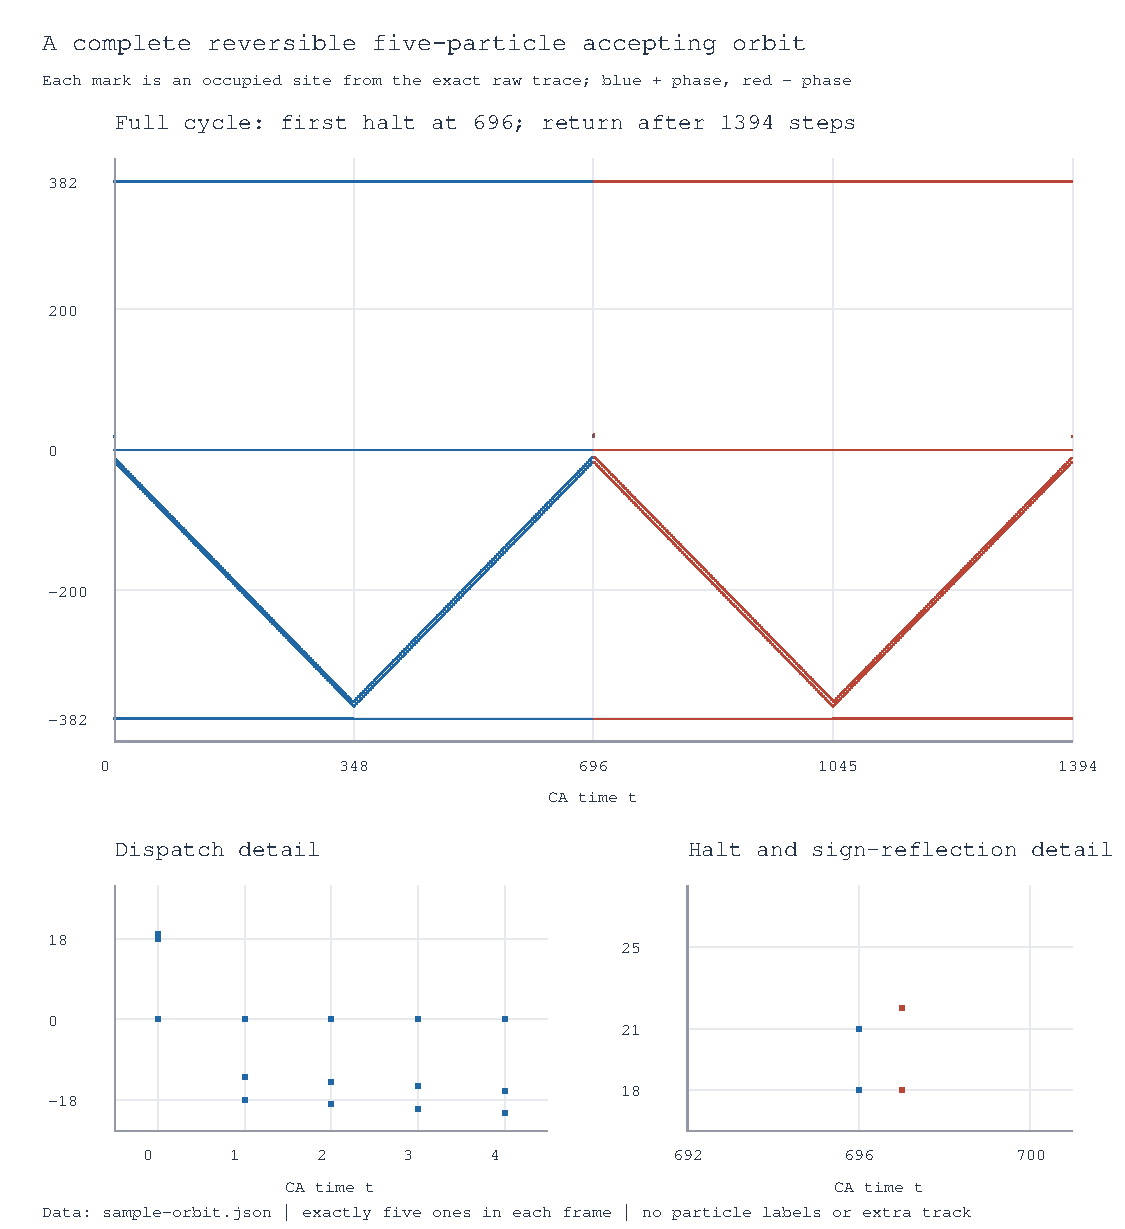
\includegraphics[width=\textwidth]{figures/accepting-orbit.pdf}
\caption{Raw five-particle space--time trace of the fully materialized
one-increment source. Every mark is drawn from the recorded occupied
coordinates; it is not an illustration inferred only from source-level
control. The large panel shows the full reflection cycle, and the detail
panels expose the close pair near dispatch and halt, where its two particles
would otherwise visually merge. The exact trace and deterministic vector
renderer are included.}\label{fpa:fig:orbit}
\end{figure}

The four explicit free/contact demonstrations cover both directions and both
boundary cases. In a departure case a triple gate acts at predecessor distance
$L$ and its reverse pair competitor is blocked at the same predecessor key.
In an arrival case a pair gate acts at predecessor distance $L+1$, with no
contact gate at that predecessor distance. These finite demonstrations support
rather than replace the general argument in Section~\ref{fpa:sec:edge}.

\section{Verification, reproducibility and limitations}\label{fpa:sec:verification}
The portable archive separates the authored article, finite compiler and
source fixtures, certificate implementation and examples, vector renderer,
and the companion lower-bound article. It requires only Python's standard
library for mathematical replay. Rebuilding the articles additionally requires
a normal \LaTeX{} installation with the packages declared in their sources.
No third-party primary-source PDF, screenshot, private working note, execution
log, bytecode cache or external dependency installation is bundled.

\wtag\ The companion lower-bound article (Report~12) is not shipped with this report: it is printed in the collection as source~17 of \path{signal-machine-collision-certificates}. The replay runner and fixtures named in this section are shipped under the prefix \path{15-rev-five-} (README).

The replay runner checks the SHA256 manifest before testing, stages mutable
outputs in a temporary directory, runs the exact checks, and compares
reproduced mathematical outputs with frozen fixtures. Its purpose is to make
the release independently executable after fresh extraction, with no absolute
workspace paths or network dependency. Generated elapsed-time measurements
are not mathematical fixtures and are not compared byte for byte.

The final independent CA executable audit comprises ten suites in ordinary
Python and again with optimization enabled. It includes $27412$ systematic
source/image predicate checks, $4448$ home-semantics checks, $1080$ independent
isolated-gate window inputs, and $835$ malformed finite inputs tested for both
inverse identities and numerical conservation. It also tests strict schema
validation, deep and cyclic Boolean syntax, constructor bypasses, immutable
snapshots, signed coordinates and exact integer domains. Runtime validation
is not implemented by assertions that disappear under optimization.

The independent certificate audit has six suites in each mode. It compares
$384$ certificate variants, $7008$ exact residual rows and $43318$ expanded
coefficients against separately built formulas; enumerates $6274$ bounded
natural/rational complete witness tuples; and rejects $556$ single-coordinate
mutations of accepted witnesses. A fractional convex mixture demonstrates
why the extra real selector-norm residual is needed. The producer's separate
suite performs $13640$ exact checks in each mode. A reinitialization loophole
in an earlier supposedly immutable certificate record was found and fixed;
the released constructors reject a second initialization before mutation, and
both audits passed the final bytes. The formulas themselves were unaffected.

Both accepting raw orbits are regenerated by full CA steps and compared with
the recorded finite fixtures. Separate independent scripts reconstruct all
$1394$ ordinary and $5670$ clean-target frames directly from the mathematics.
The certificate CLI regenerates natural and paid-real ordinary and clean
artifacts and compares each polynomial and witness byte for byte. The vector
renderer regenerates its PDF and SVG from the raw ordinary trace.

The independent isolated-swap proof establishes reversibility on the infinite
full shift. A periodic-ring exhaustive check corroborates it for one tiny
instance: all $2^{17}=131072$ binary inputs with support-radius parameter
$B=1$ were tested, and $3060$ change. Every case preserves raw keys,
eligibility, mass and the square-identity law. This is finite corroboration,
not an exhaustive check of the general theorem.

The independent geometric compiler stress test uses $m=5,p=4,a=1,J=2$ and
$954$ gates. It checks $31957$ source-path microedges, $63914$ signed endpoint
checks and $250$ signed homes. Its deliberately merging target control has
disjoint \emph{actual} image predicates; it also tests decrement on both
sides, stuck states, image gaps, interaction endpoints and the free/contact
boundary. These checks isolate potential geometric and predicate errors,
but neither this finite source nor the accepting example proves universal
source existence.

The release's claims have four distinct supports: the all-input mathematical
lemma, the admissible simulation proof, the classical universal-source theorem,
and reproducible finite implementation checks. None is silently used in place
of another. The software is an audited research implementation, not a certified
proof assistant extraction. The mathematical audit does not certify a literal
universal source table that is absent from the release.

\section{The five-particle threshold and relation to earlier work}\label{fpa:sec:threshold}
The companion Report 12 proves a separate four-mass decision theorem for fixed
one-dimensional finite-alphabet conservative CAs with a unique zero-weight
vacuum, positive integer nonvacuum weights, and at most one weight-one symbol.
For mass at most four, exact finite-configuration reachability and finite-pattern
occurrence, anchored or anywhere, are decidable. Its proof handles translating
packets and expanding shuttles rather than assuming timed semilinearity.
It is included with its original \LaTeX{}, PDF and vector figure
byte-preserved~\cite{fpa:report12}.

\begin{corollary}[Matched binary reversible particle threshold]\label{fpa:cor:threshold}
Taking the separate four-mass decision theorem as proved in the companion,
five is the least number of ones allowing undecidable effective finite-input
halt-pattern occurrence or exact finite-target reachability for a fixed
one-dimensional globally reversible, number-conserving binary CA of arbitrary
finite radius. For exact reachability, both the initial and target
configurations are computable functions of the input.
\end{corollary}
\begin{proof}
The companion applies to all binary conservative CAs and hence to their
reversible subclass, excluding a computable halting reduction at mass at most
four. Corollary~\ref{fpa:cor:universal} gives such a reduction with exactly five
ones. Corollary~\ref{fpa:cor:exact} supplies the five-particle exact-target upper
bound, and the same companion supplies its mass-at-most-four lower bound.
All statements use finite zero-background inputs and their specified local
observations or exact finite targets.
\end{proof}

This matched statement explicitly depends on two proofs. The upper construction
does not reprove the four-mass theorem. The companion's numerical four-mass
statement is broader in alphabet and does not by itself provide the binary
upper bound. Its byte-preserved version predates the present reversible binary
upper construction, so its discussion of that previously open part is read
in that chronological context.

\wtag\ Report~12 is source~17 of \path{signal-machine-collision-certificates} (Part~VI, Theorem \path{smc:fm:thm:main}); it arrived in batch~80, a day before this report. Its statement that a binary five-particle upper bound was open is answered by this Part: Report~14 (second half of this Part) and the present Report~15 each supply it.

Morita--Imai's 2001 construction provides a finite-zero-background,
number-conserving reversible simulation with a numerical triple-part alphabet;
its reported mass depends on the source-control count~\cite{fpa:moritaimai2001}.
Morita's 2012 construction gives a one-dimensional reversible
number-conserving CA with $96$ numerical states, but its discussed universal
configurations have an infinite ultimately periodic background~\cite{fpa:morita2012}.
Neither statement alone is a binary five-one construction. These are relevant
precedents, not inputs to the isolated binary-swap proof.

The 2016 article by Alhazov and Imai is directly relevant to particle
complexity~\cite{fpa:alhazovimai}. Its full construction was not available in
the targeted source review used here, so no inference about its exact binary,
reversible or optimality scope is made. An unsuccessful or incomplete search
is not a novelty or priority argument. No claim of being the first such
construction is made in this report.

\section{Research questions and sharpenings}\label{fpa:rep:15:last}
The construction raises concrete questions that do not affect the established
bounds:
\begin{enumerate}
\item \textbf{Literal universal source.} Materialize and independently audit a
universal reversible two-counter table in the accepted schema. This would turn
symbolic $m,p,a,J$ into numerical universal parameters and permit end-to-end
source-level replay of a chosen encoded computation.
\wtag\ Answered by Part~\ref{fpa:part:two} (Report~16): a literal universal reversible table in this schema, with $m=122{,}622$, $p+a=141{,}561$ and $J=0$, its clean loader and all-input proofs. End-to-end source-level replay of a universal computation remains out of reach (Report~16 predicts about $8\cdot10^{13}$ source steps for empty-tape initialization; Report~17 reduces that startup to 138 executed steps).

\item \textbf{Radius and gate optimization.} The sum-of-factor bound is
intentionally generous. Can one reuse gap codes, reduce isolation halos, or
prove a smaller composed dependency cone without losing all-input reversibility?
Can the fixed five-particle construction be made near a useful minimal radius?
\item \textbf{More economical certificates.} Finite class normalization can
multiply branch count by $(J+2)^2$. Can a direct guard-circuit encoding preserve
a unique natural witness fiber with fewer residuals and controlled degree?
\item \textbf{Uniform versus bounded arithmetization.} The horizon here is
compiled syntax. A single horizon-free polynomial representing the same
unbounded reachability relation would require an additional genuine uniform
arithmetization theorem, not a reinterpretation of these bounded certificates.
\item \textbf{Mechanized proof.} Formalize the all-input raw-key invariance
lemma, enabled-edge admissibility, and signed matching construction in a proof
assistant; relate the executable sparse-set implementation to its local-rule
semantics.
\item \textbf{Conservation and small-particle lower bounds.} Examine how the
separate four-mass analysis changes with multiple distinguishable unit labels,
nonuniform schedules, higher-dimensional lattices or active zero-weight
backgrounds. The current threshold does not cover those different models.
\end{enumerate}

\reportopening{14}{Five particles in a binary conservative cellular automaton}{}{An explicit counter compiler and finite horizon Diophantine certificates}

\begin{reportabstract}{14}
Every finite deterministic two-counter program with increment and conditional
decrement compiles effectively to a fully specified one-dimensional binary
conservative cellular automaton. Every valid simulation uses exactly five
occupied sites. Finite geometric gap codes carry control; two unbounded gaps
carry counters. A read-only remote zero sensor and strictly bounded component
writes make the rule conservative on arbitrary binary configurations, including
malformed inputs. The proof supplies a finite radius, exact instruction clocks,
and a finite anchored halt word with no premature occurrences.

A pinned 8,408-instruction universal source gives alphabet size two, radius
756,787 and halt-word length 50,452. Its guarded component description has
1,272,679,260 indexed cases. The binary truth table has $2^{1,513,575}$ input
rows and is specified algorithmically, not materialized. Universality uses the
independently checked finite-input Neary--Woods source and all-input
Turing-machine-to-counter proofs, rather than an inference from table size.
Together with the separately proved mass-four decision theorem in companion
Report 12, this gives a sharp five-particle threshold in the stated binary
finite-input halt-observation model.

For each syntactically fixed literal-source horizon $h$, an explicit ordinary
sum-of-squares polynomial has $10,750h$ natural witness variables,
$2,344h+1$ squared residuals and degree at most four. Its complete witness fiber
is empty or a singleton. Exact CA time costs one further variable and square;
a paid nonnegative-real variant costs one further square per source step.
Natural external inputs, the prime-encoded loader, enormous geometric
constants and expansion costs are all retained. This is a mathematical proof
with executable audits, not a proof-assistant formalization or a priority claim.
\end{reportabstract}

\wtag\ Delivered as \path{five-particle-binary-portable.zip} (batch~82, archive~23; arrival \texttt{db37d18c8}), dated 3~October 2026; files placed by \texttt{bca6383e9} with the prefix given in Appendix~\ref{fpa:app:provenance}. Report~14 is unnumbered in its own header; Report~16's compiler proof identifies it (``Report~14's nonreversible 8408-row source''). It and Report~15 were written about forty minutes apart and neither cites the other; Report~15's Corollary~\ref{fpa:cor:threshold} implies Report~14's Corollary~\ref{fpa:bc:cor:sharp} (note after it). Both are printed in full, since their compilers, classes and universal instances differ.

\section{The model and the result}\label{fpa:rep:14:first}
A binary configuration is a function $x:\Z\to\{0,1\}$. Its occupied set is
$X=\{i:x(i)=1\}$. When $X$ is finite, its mass is $|X|$; thus a particle here
is exactly one occupied lattice site, without a hidden color, weight or label.
A radius-$R$ cellular automaton (CA) is determined by a Boolean function
$f:\{0,1\}^{2R+1}\to\{0,1\}$, with
$F(x)(i)=f(x(i-R),\ldots,x(i+R))$. Its radius need not be minimal.
We require the all-zero vacuum to be fixed and mass to be conserved on every
finite-support input. We also give a full-shift transport interpretation,
where total cardinality need not be finite.

A source program has a finite set $Q$ of controls, an entry control $q_0$, a
distinguished halt control $q_*$ with no outgoing row, and two counters
$a,b\in\N=\{0,1,2,\ldots\}$. Every other control has one row:
\[
\begin{array}{lll}
\ADD(j,q') &: & c_j\gets c_j+1,\quad q\gets q',\\
\SUB(j,q_+,q_z) &: &
  c_j>0:\ c_j\gets c_j-1,\ q\gets q_+;\qquad
  c_j=0:\ q\gets q_z,\\
\NOP(q') &: & q\gets q'.
\end{array}
\]
Here $c_0=a,c_1=b$ and $j\in\{0,1\}$. The optional no-operation row is
included for convenience. All destinations are defined controls; self-loops
are allowed. The implementation orders control labels lexicographically,
with the halt control placed last. Control labels are finite strings, and
the supplied source table is held fixed after compilation.

\begin{theorem}[Binary five-particle compiler]\label{fpa:bc:thm:compiler}
From every such finite source program one can effectively construct a fixed
binary finite-radius CA $F$, a computable finite-input encoding
$\Enc(q,a,b)$ of mass exactly five, and a fixed finite binary word $w_*$ anchored
at the origin, with the following properties.
\begin{enumerate}
\item $F$ is defined on the whole binary shift and conserves every finite-support
configuration. Every valid simulation has exactly five particles at every tick.
\item There is an exact positive integer duration for each nonhalting source
step. The CA reaches the encoding of its source successor after that duration.
Iterating gives exact simulation of every finite or infinite source run.
\item On every valid encoded orbit, $w_*$ occurs at its fixed anchor precisely
when a committed source halt configuration has been reached. The first
occurrence time is the sum of the exact source-step durations. Halt persists.
\end{enumerate}
\end{theorem}

The theorem states a simulation of sequential source computations. It does
not assert reversibility, intrinsic universality, efficient input preparation,
efficient CA time, or minimal radius. The proof is independent of whether the
chosen source program is universal. Section~\ref{fpa:bc:sec:universal} supplies a
particular universal instance with a separately checked provenance chain.
Section~\ref{fpa:bc:sec:lower} then combines this upper bound with a separate lower
bound in an exactly matched model.

\section{Finite codes and buffered geometry}\label{fpa:bc:sec:geometry}
Let $m=|Q|$, let $p$ be the number of $\ADD$ or $\SUB$ rows, let $n$ be the
number of $\NOP$ rows, and let $z$ be the number of $\SUB$ rows. Thus
$m=p+n+1$. Make one home code $H_q$ for each control and one outbound code
$O_q$ and inbound code $I_q$ for each moving control. Give these codes distinct
integer gaps, first all home codes, then all outbound codes, then all inbound
codes, in the specified control order. Write $d(\cdot)$ for this bijection
onto $\{1,\ldots,D\}$, where
\begin{align}
D&=m+2p,& C&=D+1,&E&=2D+2,\label{fpa:bc:eq:constants1}\\
K&=4D+5=2E+1,&Z&=4K,&R&=Z+3K+E=30D+37.\label{fpa:bc:eq:constants2}
\end{align}
The constants have distinct functions. $D$ bounds a packet's internal gap;
$C$ separates it from a marker; $E$ bounds the write enlargement; $K$ defines
components and contact; $Z$ is the counter buffer and zero-read distance;
$R$ is the sufficient local radius.

For a marker at $o$, a side $s\in\{-1,+1\}$ and a gap code $d$, define
\[
 \mathcal P(o,s,d)=\{o+sC,\ o+s(C+d)\}.\label{fpa:bc:eq:pair}
\]
This is a two-particle packet. Its two particles have no separate labels.
The valid source-boundary encoding is
\begin{equation}
 \Enc(q,a,b)=\{-(Z+a),\ 0,\ Z+b\}\ \cup\ \mathcal P(0,+1,d(H_q)).
 \label{fpa:bc:eq:encoding}
\end{equation}
The outer left marker encodes $a$, the outer right marker encodes $b$, and
0 is the origin marker. These names describe an invariant of valid runs;
they are not extra states available to the binary local rule.

All five coordinates in \eqref{fpa:bc:eq:encoding} are distinct: the close packet is
strictly right of 0, its furthest site is at most $C+D=2D+1<Z$, and both outer
markers lie at distance at least $Z$ from 0. The only adjacent occupied gap
at most $D$ is the packet gap. Every unspecified site is exactly zero.
Translation of the encoding simply translates the whole future and its
observer anchor. For definiteness, inputs use origin 0.

If $q$ acts on counter $j$, put $s_q=-1$ when $j=0$ and $s_q=+1$ when $j=1$.
The travel direction of $O_q$ is $s_q$, and that of $I_q$ is $-s_q$.
Direction is recovered from a geometric code and the fixed source table;
it is not stored as a separate particle property.

\section{The complete rule on arbitrary configurations}\label{fpa:bc:sec:rule}
Join consecutive occupied sites when their distance is at most $K$.
The resulting maximal connected occupied sets are called components.
For an infinite configuration, components may be finite, infinite in one
direction, or infinite in both directions. Empty regions contain no component.
Every component is left fixed unless one of the rules below applies.
In particular, singletons, components of size at least four, and infinite
components are all frozen.

A three-particle component is eligible only if exactly one of its two adjacent
gaps is at most $D$ and the other adjacent gap is in $[C,K]$. The close pair is
the packet and the remaining particle is the marker. This parsing is unique
because $C=D+1>D$. Denote the marker by $o$, the packet by $P$, its internal
gap by $d$, and its nearest distance to the marker by
$a=\min_{x\in P}|x-o|$. In particular, no triple with two close gaps is parsed
as two competing packets.

\subsection{Free travel and departure}
For a two-particle component with gap $d(O_q)$ or $d(I_q)$, translate both
particles by one site in the recovered travel direction. A home-coded pair
is fixed. Any pair without a recognized travel code is fixed.

In an eligible travel triple, let $v\in\{-1,+1\}$ be its travel direction.
The marker is \emph{behind} the packet when
\[
 (v=+1\text{ and }o<\min P)\quad\text{or}\quad
 (v=-1\text{ and }o>\max P).
\]
In that case fix the marker and translate the packet by $v$, for every
$a\in[C,K]$. If the marker is ahead, do nothing unless $a=K$; the contact
rules below cover exactly that case. An ahead marker at distance less than
$K$ freezes. Such malformed cases need not simulate anything, but have a
well-defined conservative evolution.

\subsection{Home dispatch and the contextual zero test}
A home triple must have the exact orientation and coordinates
\[
 \{o,\ o+C,\ o+C+d(H_q)\}.
\]
Other arrangements carrying a home gap freeze. The home rules retain $o$:
\begin{enumerate}
\item For $\ADD(j,q')$, replace the packet by
$\mathcal P(o,s_q,d(O_q))$.
\item For $\SUB(j,q_+,q_z)$, inspect the old binary value at $o+s_qZ$.
If that value is one, replace the packet by
$\mathcal P(o,+1,d(H_{q_z}))$. If it is zero, dispatch
$\mathcal P(o,s_q,d(O_q))$.
\item For $\NOP(q')$, replace it by $\mathcal P(o,+1,d(H_{q'}))$.
\item For $q=q_*$, leave the component fixed.
\end{enumerate}
The contextual inspection is a read of the old global configuration. It does
not move or erase the sensed site, does not reserve its component, and does
not change the component partition. All components are updated simultaneously
from the same old configuration.

\subsection{Endpoint reversal and home commit}
Consider an ahead-marker contact at distance exactly $K$.
For code $O_q$, write $s=s_q$ and
\[
 \Delta_q=\begin{cases}+1,&q\text{ is }\ADD,\\-1,&q\text{ is }\SUB.\end{cases}
\]
Move the contacted marker to $o'=o+s\Delta_q$, and replace the packet by
$\mathcal P(o',-s,d(I_q))$. This reverses the packet on the inner side of
the updated endpoint. On valid runs the decrement case was dispatched only
when the selected counter was positive.

For code $I_q$, retain the contacted marker $o$ and put the packet at
$\mathcal P(o,+1,d(H_{q_+}))$, where $q_+$ denotes the $\ADD$ successor or
the positive $\SUB$ successor. In a left-counter excursion this final rewrite
may carry the packet across the origin marker. The marker itself remains fixed.
All unlisted cases freeze.

\begin{lemma}[Deterministic parsing]\label{fpa:bc:lem:parse}
These rules assign exactly one output set to every component in every binary
configuration, without a promise of valid encoding.
\end{lemma}
\begin{proof}
Component sizes separate pair rules from triple rules. An eligible triple has
one uniquely selected close pair and one marker. Its positive gap selects
exactly one code among the disjoint $H$, $O$, and $I$ code ranges. Home geometry
has a specified orientation and distance. Travel direction is fixed by the
code; ahead and behind are exclusive. A contact requires precisely $a=K$.
Finally, the two home $\SUB$ alternatives read the same old bit and have
complementary guards. No case requires a priority ordering between competing
rewrites. Every remaining configuration is covered by the freeze convention.
\end{proof}

\section{Conservation with remote reads and bounded writes}\label{fpa:bc:sec:conservation}
The zero sensor can lie in a different component, whose own update can be
unrelated to the computation. This is the reason to separate reading distance
from writing distance. Conservation depends on a uniform bound on the latter,
not on independence of the former.

\begin{lemma}[Equal cardinality and bounded output hull]\label{fpa:bc:lem:hull}
For every finite component $A$, its replacement $A'$ has $|A'|=|A|$ and
\[
 A'\subseteq[\min A-E,\max A+E].
\]
The statement holds for either value of every contextual guard.
\end{lemma}
\begin{proof}
Frozen components retain all their sites. A translated pair retains two
distinct sites. Every rewritten triple consists of a marker and a pair with
positive internal gap and marker-to-pair distance at least $C>D$, hence has exactly
three distinct sites.

Free and departure translations enlarge the hull by at most one. A changed
home gap enlarges it by at most $D$. A dispatch to the opposite side or a
return commit across the marker has new coordinates of absolute marker
relative value at most $C+D=2D+1<E$.

At an outbound contact the old near packet site lies $K$ on the inner side of
the marker, and the far site is another $d(O_q)$ inward. The new marker moves
by one, while both new packet sites are on its inner side within $C+D$.
The inequalities $K>C+D$ and $K>C+2D+1$ put the new inner pair between the old
far extent and the marker, allowing the marker's one-site enlargement.
Thus the coarser common allowance $E$ covers every case. Both zero-test
outcomes satisfy the same estimate, regardless of what caused the read bit.
\end{proof}

\begin{proposition}[Global numerical conservation]\label{fpa:bc:prop:cons}
The component rule conserves mass on every finite-support binary configuration.
\end{proposition}
\begin{proof}
Two distinct old components have occupied endpoint separation greater than
$K$. Their closed output-hull allowances enlarge toward each other by at most
$2E$, whereas $K=2E+1$. The enlarged lattice intervals are therefore disjoint.
This includes intervals around frozen components. Consequently output sites
from different components cannot collide or overwrite retained sites.
Summing the cardinality equality of Lemma~\ref{fpa:bc:lem:hull} over components gives
$|F(X)|=|X|$. No valid-input invariant entered the proof.
\end{proof}

For example, two malformed home triples may simultaneously read
the same remote particle. Those reads may all select a misleading zero branch.
Each selected rewrite still preserves its own cardinality and stays in its
private bounded output allowance. Shared reads do not consume the particle,
so they cannot create or destroy mass. Dense components and ambiguous packets
are frozen instead of being resolved by an unproved global scheduler.

There is also a useful full-shift formulation. Match old and new particles
in increasing order within each changed component; match frozen particles to
themselves. Each changed component has diameter at most $2K$, so its matching
has displacement at most $2K+E$. Disjoint enlarged hulls make the union a
bijection from the old occupied set to the new occupied set, for arbitrary
infinite as well as finite configurations. This matching is translation
equivariant. On a periodic configuration it descends to a bijection of occupied
site orbits modulo the spatial period, proving per-period conservation.
This is a transport statement, not an assertion that the CA map itself is
injective or reversible.

\section{A finite local rule and its radius}\label{fpa:bc:sec:locality}
A component definition is not automatically a local rule: in particular, the
instruction to freeze an infinite or very large component must be locally
indistinguishable from the appropriate finite cases. We verify that the
claimed radius covers both the positive detection and this exclusion issue.

\begin{lemma}[Local determination]\label{fpa:bc:lem:local}
The output bit at $i$ is determined by the old word on $[i-R,i+R]$, with
$R=Z+3K+E$ from \eqref{fpa:bc:eq:constants2}.
\end{lemma}
\begin{proof}
A component that can change or supply the output at $i$ has at most three
particles. By Lemma~\ref{fpa:bc:lem:hull}, its old hull is within $E$ of $i$, and its
diameter is at most $2K$. Thus all its particles are within $E+2K$ of $i$.
To certify that it is an entire component, inspect the $K$ sites just beyond
each endpoint. These boundary guards are within $E+3K$ of $i$. Any contextual
home read is at distance at most $Z$ from its marker, hence within $E+2K+Z$
of $i$. Both bounds are at most $R$.

Conversely, a large component containing a relevant occupied site cannot be
misread as a small one merely because the observed word is truncated.
If it contains at least four particles, four consecutively connected
particles including that site can be exposed within distance $3K$ of it.
Equivalently, if a purported size-two or size-three component of the truncated
word could change the central output, the preceding bounds put \emph{both}
its complete $K$-wide boundary guards strictly inside the observation window.
It therefore has no hidden continuation outside that window. Components whose
only observed fragments lie near the window endpoints cannot write at $i$,
by the same diameter and hull allowance. For a central occupied site in a
frozen large component, the four-site witness certifies that it stays occupied.
An empty central site can acquire a particle only through one of the completely
visible small components. This handles retention as well as creation of the
central bit and proves equality with the full-configuration definition.
\end{proof}

A literal Boolean evaluator is now specified: given the exact radius-$R$ word,
regard its ones as a finite set of occupied offsets, partition them into
$K$-components, apply Section~\ref{fpa:bc:sec:rule} using the supplied old word, and
return one exactly when its output contains offset zero. The code
\texttt{BinaryCA.local} implements this finite algorithm. Absent offsets in
the supplied window mean exact zeros; offsets outside the window are rejected.
Lemma~\ref{fpa:bc:lem:local} proves that this evaluator agrees with the full-shift
map. Translation equivariance and time independence follow from the rule's
relative-coordinate definition. The vacuum is fixed.

The count of Boolean inputs is exactly $2^{2R+1}$. A finite program that
terminates on every one of those inputs completely specifies the local table.
This release does not enumerate that bit string. The sparse component evaluator
is a convenient way to compute selected local outputs and whole finite traces;
it is not a different state space or an extra oracle outside the CA.

\section{The all-input simulation proof}\label{fpa:bc:sec:simulation}
We now restrict to valid encodings. The source counters may be arbitrarily
large natural numbers; none of the proof depends on a finite test range.

\begin{lemma}[Packet and marker separation]\label{fpa:bc:lem:separation}
Throughout a valid source excursion, the packet has internal gap at most $D$,
there is exactly one close pair, and it cannot belong to a component containing
two distinct markers. All other components are isolated markers.
\end{lemma}
\begin{proof}
At a source boundary the markers are at $-(Z+a),0,Z+b$ and their consecutive
separations are at least $Z$. Home and travel codes all have gaps in $[1,D]$.
A two-site packet can connect two markers by gaps at most $K$ only if their
separation is at most $2K+D$. But $Z=4K>2K+D$. Endpoint addition increases
its separation from the origin; positive decrement reduces it to no less
than $Z$. The origin stays fixed, and both reversals and home commits place
an intact coded packet at distance at least $C>D$ from their marker.
Translations preserve its internal gap. These facts propagate the asserted
separations through every phase.
\end{proof}

\begin{lemma}[Exact home zero test]\label{fpa:bc:lem:zero}
At a valid home configuration with selected counter $c$ and side $s$, the old
bit at $sZ$ is one if and only if $c=0$.
\end{lemma}
\begin{proof}
The selected endpoint is at $s(Z+c)$, so it occupies $sZ$ precisely when
$c=0$. The other endpoint is on the opposite side, the origin is at zero,
and the entire home packet is within $C+D<Z$ of zero. No other valid particle
can occupy the tested site. Thus dispatch of a decrement excursion implies
$c\ge1$; it can never decrement below the buffer.
\end{proof}

\subsection{Exact microstates of an arithmetic excursion}
Fix a moving control $q$, selected old counter $c$, side $s=s_q$, and change
$\Delta=+1$ for addition or $-1$ for positive decrement. Put
\begin{align}
 d_O&=d(O_q),&d_I&=d(I_q),\\
 L_O&=Z+c-K-C-d_O,&
 L_I&=Z+c+\Delta-K-C-d_I.\label{fpa:bc:eq:flights}
\end{align}
The untouched endpoint stays fixed throughout. After the dispatch tick the
packet is $\mathcal P(0,s,d_O)$. After $u$ subsequent travel ticks,
$0\le u\le L_O$, it is
\begin{equation}
 \{s(C+u),\ s(C+d_O+u)\}.\label{fpa:bc:eq:outstate}
\end{equation}
Its separation from the origin initially equals $C$ and grows one site at a
time. It first uses the behind-marker rule, then the free-packet rule. At
$u=L_O$ its leading site is exactly $K$ from the selected endpoint
$s(Z+c)$. Integer unit motion cannot skip this contact. Before then its
ahead distance is greater than $K$, so there is no early reversal.

The next tick moves the endpoint to $o'=s(Z+c+\Delta)$ and places the inbound
packet at $\mathcal P(o',-s,d_I)$. After $v$ return travel ticks,
$0\le v\le L_I$, its sites are
\begin{equation}
 \{o'-s(C+v),\ o'-s(C+d_I+v)\}.\label{fpa:bc:eq:instate}
\end{equation}
Again it departs a behind marker, travels freely, and then contacts the origin
at distance $K$, exactly at $v=L_I$. Its next tick commits the successor home
code. The resulting configuration is
$\Enc(q_+,a+\Delta,b)$ for the left counter and
$\Enc(q_+,a,b+\Delta)$ for the right counter.

The travel lengths are strictly positive even at the smallest counters:
\[
 L_O\ge Z-K-C-D=3K-C-D>0,
\]
and, using $c+\Delta\ge0$ in the decrement case,
$L_I\ge3K-C-D>0$. Thus the formulas include departure, separation and contact
without a zero-length ambiguity. At every intermediate phase the packet lies
between the two outer markers. The origin-crossing commit also remains there.

\begin{proof}[Proof of Theorem~\ref{fpa:bc:thm:compiler} apart from observation]
The whole-shift CA and conservation assertions follow from
Proposition~\ref{fpa:bc:prop:cons} and Lemma~\ref{fpa:bc:lem:local}. At a home state,
Lemma~\ref{fpa:bc:lem:zero} selects the correct zero branch or arithmetic excursion.
The explicit microstates \eqref{fpa:bc:eq:outstate}--\eqref{fpa:bc:eq:instate} and
Lemma~\ref{fpa:bc:lem:separation} show that all intermediate rules apply exactly as
claimed and that the endpoint update changes only the selected counter.
A zero decrement or no-operation instead commits its stated successor in one
tick. A halt encoding is fixed. Induction over source steps proves the
source-boundary invariant for arbitrary natural inputs. Because every
nonhalting source instruction has a finite positive duration, any infinite
source run produces an infinite CA run with all its source boundaries reached.
Global conservation keeps mass exactly five at every intermediate tick.
\end{proof}

\section{Exact clocks and the anchored halt word}\label{fpa:bc:sec:clock}
An arithmetic excursion consists of one dispatch, $L_O$ translations, one
endpoint reversal, $L_I$ translations and one home commit. Therefore its
exact duration is
\begin{equation}
 \tau_q(c)=3+2(Z+c)+\Delta_q-2K-2C-d(O_q)-d(I_q)
          =2c+\kappa_q,\label{fpa:bc:eq:clock}
\end{equation}
where
$\kappa_q=3+2Z+\Delta_q-2K-2C-d(O_q)-d(I_q)$.
Zero decrements and no-operations take exactly one tick. A state already halted
has first-halt time zero, and its future configuration is fixed.

Define a finite word $w_*$ on the integer interval $[0,C+D]$ by requiring ones
exactly at
\begin{equation}
 0,\quad C,\quad C+d(H_{q_*}),\label{fpa:bc:eq:observer}
\end{equation}
and zeros at \emph{every} other site of the interval. Its length is
$C+D+1=2D+2=E$. No counter value appears in this word.

\begin{proposition}[No false or early halt observation]\label{fpa:bc:prop:halt}
On the orbit of any valid encoding, the anchored word $w_*$ occurs if and only
if a committed source halt has been reached. Its first occurrence is at the
sum of the durations \eqref{fpa:bc:eq:clock} and the unit zero/no-operation durations
along the first-halt source trace.
\end{proposition}
\begin{proof}
Both endpoints remain outside the observer window. The three prescribed ones
must therefore be the origin and the packet. Their only close pair has gap
$d(H_{q_*})$. At every intermediate time there is exactly one close pair,
and every outbound and inbound code has a different gap. The halt gap also
differs from every other home code. Hence an excursion whose \emph{future}
source successor is halt cannot exhibit the word before the home commit.
At a committed home state the packet has the exact positive-side geometry
of \eqref{fpa:bc:eq:observer}, and the word appears precisely for control $q_*$.
The required zeros hold because no additional particle lies in the window.
The halt rule is the identity, so the word then persists. Summing the exact
step clocks gives its first occurrence time.
\end{proof}
This completes Theorem~\ref{fpa:bc:thm:compiler}. The observation is anchored and
finite. It is not an exact finite-configuration target test: the two final
counter endpoints can be arbitrarily far away and can encode arbitrary final
counter values. Conversely, conservation does not weaken the observer's zero
requirements; they are essential parts of the finite word.

\section{Exact finite description counts}\label{fpa:bc:sec:counts}
Before removing identity cases or cases unreachable from valid encodings,
the complete component scheme has the following indexed guarded cases:
\begin{center}
\begin{tabular}{lr}
\toprule
Rule family&Number of indexed cases\\
\midrule
Free outbound and inbound packet translation&$2p$\\
Behind-marker departure for every $a\in[C,K]$&$2p(K-C+1)$\\
Ahead-marker endpoint contact and home contact&$2p$\\
Home dispatch or commit, splitting each zero read&$p+n+z$\\
\midrule
Total&$4p+2p(K-C+1)+p+n+z$\\
\bottomrule
\end{tabular}
\end{center}
Every SUB has two complementary home guard alternatives, which accounts for
the extra $z$ beyond the number of nonhalting controls. Each travel code has
one permitted behind orientation and one ahead orientation, so no uncharged
direction label is missing. The otherwise-frozen convention is part of the
finite rule definition.

These are counts of an indexed component schema. This release stores the
finite algorithm and its source table, not one written record for every
indexed component case. In particular, neither this schema count nor the
number of source instructions is the number of Boolean local-table rows.
The latter is exactly $2^{2R+1}$. Given a neighborhood, the algorithm fixes its
central output in finite time, so the distinction is representational rather
than a missing rule or unspecified behavior.

\section{The pinned universal source}\label{fpa:bc:sec:universal}
\wtag\ \textbf{A second presentation.} The 8,408-row source of this section is the prime-coded program of quadratic-orthant-certificates (QOC) Part~V, source~16 (its \S\path{qoc:um:sec:virtual} and \S\path{qoc:um:sec:prime}); the 528-row three-counter program, the stack invariants with cost $5Q+r+7Y_0+w+4$, the prime macros with cost $(3p+1)N+2$, the row count 8,408 and the verifier's 4,475 symbolic paths are proved there as Lemmas \path{qoc:um:lem:virtual} and \path{qoc:um:lem:prime}. Report~14 shipped that report's \texttt{verify\_source.py} and receipt byte for byte; they are not shipped again. The section is kept in full, as Report~14's own route to the same lemmas, because Report~14's universal instance and its counts depend on it; no novelty is claimed for it.

The generic theorem becomes a universal CA only after a universal source is
supplied and its input interface is matched to the encoding. The delivered
source has 8,408 literal two-counter instructions, comprising 6,068 ADD rows
and 2,340 SUB rows, with 8,409 controls including halt. All aliases and
instruction macros have been expanded. Its exact bytes are pinned in the
portable source-verification dependency. Row count alone establishes none
of its semantic or universality properties.

\subsection{The finite-input primary machine}
The primary reference is T.~Neary and D.~Woods,
\emph{Four Small Universal Turing Machines}, \emph{Fundamenta Informaticae}
\textbf{91} (2009), 105--126, DOI 10.3233/FI-2009-0008~\cite{fpa:nw}.
Equation (3), Definition 3.1 and Table 1 give effective finite program/data
encodings with blank tails, start control $u_1$, and scanned blank $c$.
Section 3.5 and Table 16 supply the corresponding 15-state, two-symbol
machine. This use is ordinary finite-input universality; it does not require
an infinite periodic background. Both finite half tapes may vary with the
encoded program and input.

The literal table uses $c=0$, $b=1$ and $u_1,\ldots,u_{15}=A,\ldots,O$.
For auditability, Table~\ref{fpa:bc:tab:tm} lists all 30 entries. Each defined entry
is (written symbol, direction, next control); undefined $J1$ is the halt.
The independently checked serialization is bundled as \texttt{tm\_table.json}.
\begin{table}[htbp]\centering
\caption{The pinned source TM, matching primary Table 16}\label{fpa:bc:tab:tm}
\begin{tabular}{ccc@{\qquad}ccc}
\toprule
Control&Read 0&Read 1&Control&Read 0&Read 1\\
\midrule
$A$&$0,R,B$&$1,R,A$&$I$&$0,R,A$&$1,L,J$\\
$B$&$1,R,C$&$1,R,A$&$J$&$1,L,K$&undefined\\
$C$&$0,L,G$&$0,L,E$&$K$&$0,R,L$&$1,R,N$\\
$D$&$0,L,F$&$1,L,E$&$L$&$0,R,M$&$1,R,L$\\
$E$&$1,R,A$&$1,L,D$&$M$&$0,L,B$&$1,R,L$\\
$F$&$1,L,D$&$1,L,D$&$N$&$0,L,C$&$0,R,O$\\
$G$&$0,L,H$&$1,L,G$&$O$&$0,R,N$&$1,R,N$\\
$H$&$1,L,I$&$1,L,G$&&&\\
\bottomrule
\end{tabular}
\end{table}

The primary scan contains a discrepancy that must remain visible. Table 16,
printed page 121 (PDF page 17), leaves $u_{10},b$ undefined. The displayed
halting configuration on printed page 123 (PDF page 19) also underlines $b$.
The prose immediately below instead says $u_{10},c$. The table and display
agree with the pinned $J1$ halt used here; the prose is recorded as inconsistent.
No author-issued erratum is asserted, and no repair to the serialized table
has been inferred. The source's old bibliography comment also gives the
incorrect page range 123--144. That comment is preserved to retain the pinned
bytes, while the report and provenance file give the verified 105--126 range.
No third-party paper or screenshot is redistributed in this package.

\wtag\ \textbf{Correction (3~October 2026).} The bibliographic details in this subsection are wrong, and the ``old bibliography comment'' is right: the publisher's record of Neary--Woods is \emph{Fundamenta Informaticae} 91(1) (2009), 123--144, DOI \path{10.3233/FI-2009-0036}, while DOI \path{10.3233/FI-2009-0008} is a different paper and 105--126 is the author-hosted PDF's own pagination (Appendix~\ref{fpa:app:provenance}, entry~\cite{fpa:nw}). The page locators ``printed page 121'' and ``printed page 123'' refer to that PDF. The $(u_{10},b)$ discrepancy is the one recorded in quadratic-orthant-certificates after its Table \path{qoc:wf:tab:tm}, and Table~\ref{fpa:bc:tab:tm} agrees with that table entry by entry.

\subsection{Finite half tapes and three natural counters}
Let $L,R$ store the finite bit stacks strictly left and right of the head,
least significant bit nearest the head; omitted high bits are blank zero.
The scanned bit is finite control, and a third register $T$ is scratch.
At a genuine TM cut, $T=0$. The literal virtual source starts at a prologue
that clears arbitrary $T$ with
\[
 \SUB(T,\text{clear},\text{first TM control}).
\]
Repeated positive branches remove one unit, followed by one failed test.
This takes $T+1$ virtual instructions and enters control $A0$.

For a defined TM transition $(q,s)\mapsto(w,D,q')$, denote the half tape in
direction $D$ by $X$ and the other half by $Y$. Write $X=2Q+r$, $r\in\{0,1\}$.
The exact stack action is
\begin{equation}
 X\gets Q,\qquad Y\gets2Y+w,\qquad T\gets0,
 \quad\text{new finite control }(q',r).\label{fpa:bc:eq:tmstack}
\end{equation}
The 528-row virtual three-counter table implements this using the following
finite ADD/SUB graphs. Their labels are distinct for each source transition
and parity branch; the delivered files contain the fully expanded rows.

The pop loop tests and decrements $X$ twice, then adds one to $T$ and repeats.
A failed first test selects remainder 0; a successful first test followed by
a failed second test selects remainder 1. After $k$ complete pair iterations,
\[
 X=2(Q-k)+r,\qquad T=k.
\]
The rank $Q-k$ strictly decreases on full iterations. At exit $X=0,T=Q$,
with $r$ in control. A transfer loop repeatedly decrements $T$ and increments
$X$ until $T=0$, producing $X=Q$. The pop stage uses exactly
$3Q+(1+r)+(2Q+1)=5Q+r+2$ virtual instructions.

To push the written symbol, drain $Y$ into $T$ at two increments of $T$ per
successful decrement of $Y$. After $k$ iterations,
$Y=Y_0-k,T=2k$, with decreasing rank $Y_0-k$. Next transfer $T$ back to $Y$
one unit at a time; its invariant is $Y+T=2Y_0$, with decreasing rank $T$.
This reaches $Y=2Y_0,T=0$. If $w=1$, one final ADD writes the low bit; if
$w=0$, the graph links directly to the next TM cut. This stage uses
$7Y_0+2+w$ virtual instructions. Consequently the full TM transition costs
\begin{equation}
 C_{\mathrm{virtual}}=5Q+r+7Y_0+w+4.\label{fpa:bc:eq:virtualclock}
\end{equation}
These invariants prove \eqref{fpa:bc:eq:tmstack} for all natural half tapes.
Every loop terminates, and none can halt internally. The undefined $J1$
transition alone reaches HALT. Induction supplies finite-prefix simulation
and halting equivalence for the complete TM run.

A repeated control label is not, by itself, a TM cut: the pop loop revisits
its first label while $T>0$. Correct replay tests the cut label \emph{and}
$T=0$. This qualification also matters at the next compilation layer.

\subsection{Three counters in two by prime coding}\label{fpa:bc:sec:prime}
At every virtual-instruction boundary the physical counters satisfy
\begin{equation}
 A=C_0\,2^L3^R5^T>0,\qquad B=0,\qquad\gcd(C_0,30)=1.
 \label{fpa:bc:eq:prime}
\end{equation}
Unique factorization gives such a representation for every positive raw
input $A$. The cofactor $C_0$ is unchanged. The prologue clears the exponent
of 5, so the raw input starts the TM with
$L=v_2(A)$, $R=v_3(A)$ and scratch zero regardless of its other factors.
No external factorization is executed by the loader or by the counter machine.
Intermediate physical $A$ may be zero; positivity is required at virtual cuts.

For a virtual ADD at prime $p\in\{2,3,5\}$, drain physical $A=N$ one unit
at a time, placing exactly $p$ increments into $B$ after each successful
SUB of $A$. After $k$ iterations,
\[
 A=N-k,\quad B=pk.
\]
The rank $N-k$ proves termination at $A=0,B=pN$. A second loop transfers $B$
one-for-one back to $A$, with invariant $A+B=pN$ and decreasing rank $B$.
It exits at $A=pN,B=0$, exactly increasing the chosen exponent. Counting
literal rows executed gives $2pN$ ADDs, $(p+1)N$ successful SUBs and two
failed SUBs, for a total
\begin{equation}
 C_{\mathrm{inc},p}(N)=(3p+1)N+2.\label{fpa:bc:eq:primeinc}
\end{equation}

For a virtual SUB, use $p$ finite remainder controls. Each successful SUB of
$A$ advances the remainder cyclically; crossing from $p-1$ to 0 additionally
increments $B$. At remainder control $j$ after $k$ complete groups,
\[
 A=N-pk-j,\quad B=k,\quad0\le j<p.
\]
Each successful test consumes a unit of $A$, so this phase terminates.
Writing $N=pQ+r$, $0\le r<p$, the failed test occurs at $A=0,B=Q$ in
remainder control $r$.

If $r=0$, transfer $B$ to $A$ one-for-one and take the positive virtual branch.
The result is $A=Q,B=0$; since $N>0$ and $p\mid N$, $Q\ge1$.
Divisibility means precisely that the chosen exponent was positive, and
division by $p$ decrements it. If $r>0$, drain $B$ with $p$ ADDs to $A$ per
successful SUB, then append $r$ further ADDs to $A$. After $k$ restoration
groups, $A=pk,B=Q-k$, so the result is $A=N,B=0$. Take the zero branch.
Nondivisibility means the exponent is zero, so this branch restores the
entire encoded state. Remainders are bounded control, never a third unbounded
physical register. All transfer ranks decrease and all continuations restore
$B=0$ before leaving the macro.

The exact SUB costs are
\begin{center}
\begin{tabular}{lrrrr}
\toprule
Remainder&ADD&Successful SUB&Failed SUB&Total\\
\midrule
$r=0$&$2Q$&$N+Q$&2&$N+3Q+2$\\
$r>0$&$N+Q$&$N+Q$&2&$2N+2Q+2$\\
\bottomrule
\end{tabular}
\end{center}
A virtual ADD uses $p+3$ literal rows. A virtual SUB uses
$(3p^2+p+4)/2$ rows, namely 9, 17 and 42 at primes 2, 3 and 5. The virtual
source has ADD counts $(74,76,145)$ and SUB counts $(58,58,117)$ on
$(L,R,T)$, including the clearing prologue. Therefore the literal row count is
\[
 74\cdot5+76\cdot6+145\cdot8+
 58\cdot9+58\cdot17+117\cdot42=8,408.
\]
The actual literal file, rather than an abstract row-count assertion, fixes
every intermediate label and destination. A physical macro cut requires its
entry label \emph{and} $B=0$, since internal drain loops can revisit that
label while $B>0$.

\subsection{What the source verifier proves}
The portable source verifier reads the saved tables and does not import the
source generator. It checks affine straight-line loop bodies such as
\[
 (A,B)=(x+p,y)\longmapsto(x,y+1)
\]
and their exits, transfers and bounded tails. Parameters are arbitrary
naturals. Every SUB on a verified path has either identically zero input or
an affine value with nonnegative coefficients and constant at least one.
Thus every selected branch and affine endpoint equality holds uniformly,
not just at sampled parameter values.

There are 4,475 checked symbolic paths, covering all 528 virtual and 8,408
literal instructions. The decreasing-rank and invariant proofs above compose
these paths into arbitrary-length terminating loops. This is the all-input
argument. Separate finite checks include 1,536 prime-macro cases, 4,698
TM/virtual cases, 261 whole TM transitions through the literal physical table,
and 81 raw-cofactor/scratch-prologue cases. Such tests supplement the proof;
they do not certify universality by extrapolation.

\subsection{The resulting fixed universal CA}
For a finite primary TM encoding, construct its natural stacks $L,R$ and use
physical input $(A,B)=(2^L3^R,0)$. Then use \eqref{fpa:bc:eq:encoding} for the fixed
literal source entry control. This is an effective finite-support encoding of
exactly five particles. Composing primary finite-input universality, the two
all-input counter simulations, and Theorem~\ref{fpa:bc:thm:compiler} gives one fixed
binary CA for which anchored halt-word occurrence is undecidable on this
computable family of finite inputs.

The exact instance has
\begin{center}
\begin{tabular}{lr@{\qquad}lr}
\toprule
Quantity&Value&Quantity&Value\\
\midrule
$m$&8,409&$p$&8,408\\
$z$&2,340&$D$&25,225\\
$C$&25,226&$E$&50,452\\
$K$&100,905&$Z$&403,620\\
Radius $R$&756,787&Observer length&50,452\\
\bottomrule
\end{tabular}
\end{center}
The component-family counts are 16,816 free cases, 1,272,634,880 departure
cases, 16,816 contact cases and 10,748 guarded home cases. Their sum is
1,272,679,260. The Boolean local truth table instead has
\begin{equation}
 2^{2R+1}=2^{1,513,575}\quad\text{input rows}.\label{fpa:bc:eq:universaltruth}
\end{equation}
Neither the billion indexed component cases nor this binary truth table is
expanded as a flat list in the archive. All of their outputs are fixed by the
small rule algorithm and pinned literal source.

The counter input can be extraordinarily large: its binary bit length is
$\lfloor L+R\log_2 3\rfloor+1$ for $A=2^L3^R$, while its geometric left
endpoint is $-(403,620+A)$. $L$ and $R$ themselves are integer values of binary
stacks, not merely their bit lengths. Prime-macro instruction costs depend on
these numeric values by \eqref{fpa:bc:eq:primeinc} and the SUB ledger; CA clock costs
depend on physical counters by \eqref{fpa:bc:eq:clock}. The construction does not
absorb the external loader into a free operation or claim a polynomial-time
map in the length of the original TM input.

\section{The sharp particle threshold and its scope}\label{fpa:bc:sec:lower}
Companion Report 12, \emph{Four mass units and exact reachability}~\cite{fpa:report12},
proves decidability of finite-pattern occurrence, anchored or anywhere, from
finite inputs of mass at most four in a broader finite weighted-alphabet model.
Its hypotheses include a unique zero-weight vacuum, positive integer weights
for other symbols, and at most one weight-one symbol. Binary occupancy satisfies
these hypotheses with weights 0 and 1. Its theorem also covers exact finite
target reachability, but the present upper bound only needs finite halt patterns.

\begin{corollary}[Sharp binary finite-input threshold]\label{fpa:bc:cor:sharp}
In the class of fixed one-dimensional deterministic finite-radius binary
conservative cellular automata with quiescent zero vacuum, five is the least
particle count permitting a computable finite-input reduction of arbitrary
Turing-machine halting to a designated finite anchored halt-pattern occurrence.
\end{corollary}
\begin{proof}
The fixed universal construction above supplies the mass-five upper bound.
If such a reduction used at most four particles, the decision procedure of
Report 12 could decide the resulting finite-pattern instance and hence the
original TM halting problem. This contradicts undecidability. The encoder is
required to be computable, so it cannot hide the undecidable answer in an
uncomputable choice of finite input.
\end{proof}

\wtag\ Corollary~\ref{fpa:cor:threshold} of Report~15 (first half of this Part) implies this corollary: a globally reversible, number-conserving binary automaton is a binary conservative automaton, so its five-particle construction is also an upper bound here, and the lower bound is the same Report~12. The two upper constructions differ: Report~14 compiles every deterministic ADD/SUB/NOP program (no injectivity needed), and gives a literal universal instance, a radius linear in $D$ and a persistent halt word; Report~15 needs partial-injective guarded sources and gives global reversibility and exact finite targets.

The all-rule mass-four classification is a separate mathematical dependency;
this article does not claim to re-prove it. Its exact authored PDF, LaTeX source
and required vector figure are included unchanged in the companion directory,
with hashes. Its original executable replay remains in its separate release.

\wtag\ Report~12 is printed as source~17 (Part~VI) of \path{signal-machine-collision-certificates}; its byte-identical companion files delivered with Report~14 are not shipped here.

The sharp statement excludes infinite initial backgrounds, active zero-weight
states, multiple unit labels, signed weights, spatially nonuniform or
 time-dependent rules, and other computational or observational models.

This matching of two proved bounds is not a claim of literature priority.
Alhazov and Imai's 2016 publisher abstract reports a five-particle universal
numerical-state NCCA~\cite{fpa:alhazovimai}; the full paper was unavailable in the
underlying review. Kong's 2021 binary thesis and Imai's 2021 project report
supply lower-particle precursors~\cite{fpa:kong,fpa:imai}. A limited targeted search
finding no reusable binary table or later resolution does not show that none
exists. The present compiler is justified by its construction, and the lower
bound by its companion proof, rather than by a present-day literature-status
inference.

\section{A source horizon polynomial compiler}\label{fpa:bc:sec:frontend}
Fix a source program and an instruction horizon $h\ge1$ as part of the
\emph{compiler syntax}. This section gives a separate ordinary polynomial for
each such $h$. For the universal instance, one unit of $h$ means one literal
ADD or SUB row of the 8,408-row two-counter program. It does not mean a TM
transition, a virtual three-counter instruction, or a CA tick. These clocks
are related by the explicit, input-dependent costs already proved.

\wtag\ \textbf{Comparison.} For the same 8,408-row source, quadratic-orthant-certificates proves a stronger certificate, Theorem \path{qoc:um:thm:poly}: degree two, $29{,}904T$ witnesses and $4T+1$ squares, exact over the naturals and over the nonnegative reals, where $T$ is the instruction horizon. The polynomial of this section has degree at most four, $10{,}750h$ witnesses and $2{,}344h+1$ squares, and needs a paid norm row for real witnesses (Section~\ref{fpa:bc:sec:real}). Report~14 did not know that theorem. What this section adds is the optional row for the automaton's clock, which ties the source horizon to the cellular-automaton time.

Expand each ADD and NOP row into one branch, and each SUB row into a positive
decrement branch and a zero branch. Let $B$ be the resulting number of branches.
Thus $B=p+n+z$. Index branches by $j=1,\ldots,B$; let $s_j,t_j$ be their
integer source and target control codes under the injective ordering
$Q\to\{0,\ldots,m-1\}$. Let $\delta_{jk}\in\{-1,0,1\}$ be the branch's
change to counter $k$. A zero or NOP branch has both changes zero. There are
exactly $z$ zero branches, and no branch starts at halt.

The initial control and natural counters $q_0,a_0,b_0$ are external inputs
or fixed constants. The actual emitter in this release specializes them to
supplied constants. The theorem-level formula also permits atomic input
coordinates, but the current emitter does not export symbolic input wires.

\subsection{All residuals and the witness variables}
For every source layer $t=0,\ldots,h-1$, introduce $B$ natural selector
variables $e_{tj}$ and two natural postcounter variables $a_{t+1},b_{t+1}$.
Use the following residuals, with $c_{t0}=a_t,c_{t1}=b_t$:
\begin{align}
 U_t&=\sum_{j=1}^{B}e_{tj}-1,\label{fpa:bc:eq:onehot}\\
 V_0&=\sum_j s_je_{0j}-q_0,\label{fpa:bc:eq:state0}\\
 V_t&=\sum_j s_je_{tj}-\sum_j t_je_{t-1,j},\qquad 1\le t<h,\label{fpa:bc:eq:state}\\
 W_{tk}&=c_{t+1,k}-c_{tk}-\sum_j\delta_{jk}e_{tj},
                         \qquad k=0,1,\label{fpa:bc:eq:counters}\\
 Z_{tj}&=e_{tj}c_{tk(j)},\qquad j\text{ a zero branch},\label{fpa:bc:eq:zeroguard}\\
 H&=\sum_j t_je_{h-1,j}-q_*.\label{fpa:bc:eq:terminal}
\end{align}
Here $k(j)$ is the counter tested by zero branch $j$. Form the ordinary
integer polynomial
\begin{equation}
 P_h=\sum_{t=0}^{h-1}\left(U_t^2+V_t^2+W_{t0}^2+W_{t1}^2+
                    \sum_{j\text{ zero}}Z_{tj}^2\right)+H^2.
 \label{fpa:bc:eq:sos}
\end{equation}
Every residual is explicitly emitted as a sparse integer polynomial. A
monomial is a list of variable indices with repetitions denoting powers;
an empty list denotes the constant monomial. No hidden integrality predicate,
exponentiation atom, branch oracle or implicit guard is part of the polynomial.
The baseline integrality condition is the stated witness domain $\N^N$.

\begin{theorem}[Exact first-halt fiber]\label{fpa:bc:thm:fiber}
For fixed natural external inputs and fixed syntactic $h\ge1$, $P_h=0$ has
exactly one complete natural witness if the deterministic source first halts
after exactly $h$ literal instructions, and has no natural witness otherwise.
\end{theorem}
\begin{proof}
A sum of real squares is zero precisely when every residual is zero.
By nonnegativity and \eqref{fpa:bc:eq:onehot}, each layer's natural selectors sum to
one and therefore exactly one of them is one. The state equations and injective
control codes force that selected branch's source to be the current control,
starting at $q_0$. The counter equations force its specified updates.

A selected zero branch has $e_{tj}=1$, so \eqref{fpa:bc:eq:zeroguard} forces its tested
old counter to be zero. A selected positive decrement at old value zero would
force its postcounter to be $-1$ by \eqref{fpa:bc:eq:counters}, which is excluded by
the natural witness domain. Thus no positive-test slack variable is needed.
ADD and NOP branches have no additional guard. Since the source is deterministic,
exactly one branch is permitted at each nonhalting state and counter pair.
Induction therefore fixes all selectors and postcounter values uniquely.

The terminal residual requires halt at layer $h$. It cannot have been reached
earlier because halt has no outgoing branch, whereas each subsequent layer
would require a branch with that source code. Hence a solution is precisely a
first-halt trace of length $h$. Conversely, any such trace supplies its one-hot
selectors and natural postcounters, making every residual vanish. Every
coordinate of that trace witness is forced, proving uniqueness of the complete
fiber, not merely uniqueness after projection to selected coordinates.
\end{proof}

\subsection{Exact dimensions and algebraic costs}\label{fpa:bc:sec:algebracost}
The unsimplified core ledger is
\begin{equation}
 \begin{aligned}
 \text{witness variables}&=h(B+2),\\
 \text{squared residual slots}&=h(4+z)+1,\\
 \deg P_h&\le4.
 \end{aligned}\label{fpa:bc:eq:coreledger}
\end{equation}
The degree-four bound comes only from squaring quadratic zero guards;
specialization can lower actual degree. A residual that becomes identically
zero remains a counted slot unless explicitly removed. Therefore slot counts
and counts of nonzero residuals are reported separately.

With initial counters treated as atomic coordinates or constants, the written
raw residual monomial occurrences before collecting like terms satisfy
\begin{equation}
 S_{\mathrm{raw}}\le h(4B+5)+2.\label{fpa:bc:eq:rawcost}
\end{equation}
Indeed the one-hot rows contribute $h(B+1)$; state rows contribute at most
$(B+1)+2B(h-1)$; the two counter rows contribute at most
$h(4+B-z-n)$; the zero rows contribute at most $hz$; and the terminal row
at most $B+1$. Their sum is $h(4B+5-n)+2$, which gives the displayed bound.
Zero coefficients, fixed input zeros and coincident terms can reduce it.

A sum-of-squares representation is an explicit representation of an ordinary
polynomial, but expansion has a real cost. If the collected residual lengths
are $\ell_1,\ldots,\ell_s$, expanding all squares by ordered products takes
at most
\begin{equation}
 \sum_{r=1}^{s}\ell_r^2\label{fpa:bc:eq:expansioncost}
\end{equation}
written term occurrences before global collection. The emitter reports the
actual lengths' sum and this expansion bound. It never charges a square as
though the fully expanded coefficients had no computational or storage cost.
The arithmetic coefficients also have bit lengths; none of these counts is
a bit-complexity claim.

\subsection{Adding exact physical time}
For branch $j$, let $\tau_j(a_t,b_t)$ equal one for a zero or NOP branch and
$2c_{t,k(j)}+\kappa_j$ for an arithmetic branch, using
\eqref{fpa:bc:eq:clock}. Add a natural witness coordinate $\Theta$ and one residual
\begin{equation}
 T=\Theta-\sum_{t=0}^{h-1}\sum_{j=1}^{B}e_{tj}\tau_j(a_t,b_t).
 \label{fpa:bc:eq:timepoly}
\end{equation}
Use $P_h+T^2$. Every summand selected by a valid trace is its proved CA duration,
so $\Theta$ is exactly the first physical halt time. It is uniquely forced.
The cost is one witness variable, one squared residual and degree still at
most four. Alternatively $\Theta$ can be a specified input coordinate; then
there is no added witness variable, and the fiber is nonempty precisely when
that time agrees with the first-halt clock.

If the source has no NOPs, the additional raw residual occurrences are at
most $h(2B-z)+1$: one selector term for each zero branch and two terms for
each arithmetic branch, plus $\Theta$. With NOPs the sharper expression is
$h(2B-z-n)+1$. Constant initial counters may combine the affine terms in the
first layer and lower the actual count.

At $h=0$, the witness-free core is simply $(q_0-q_*)^2$; first physical halt
time, when defined, is zero. The actual emitter's optional unsimplified clock
version retains one $\Theta$ witness and two residual slots,
$(q_0-q_*)^2+\Theta^2$. Substituting the known value $\Theta=0$ removes that
witness. Neither convention is silently charged as the other.

\subsection{Numerical height and space bounds}\label{fpa:bc:sec:bounds}
Put $M=\max(a_0,b_0)$ and
$\kappa_{\max}=\max(1,\max_{q\text{ moving}}\kappa_q)$, taking the inner
maximum absent when there are no moving rows. In any valid $h$-instruction
trace,
\begin{align}
 0\le a_t,b_t&\le M+h,\label{fpa:bc:eq:height}\\
 \Theta&\le h(\kappa_{\max}+2M)+h(h-1),\label{fpa:bc:eq:timebound}\\
 \diam\left(\bigcup_{0\le u\le\Theta}\supp F^u(\Enc(q_0,a_0,b_0))\right)
 &\le2Z+a_0+b_0+h.\label{fpa:bc:eq:diambound}
\end{align}
For \eqref{fpa:bc:eq:height}, a counter increases by at most one per source instruction.
At layer $t$ its old value is at most $M+t$, giving duration at most
$\kappa_{\max}+2(M+t)$ even for unit-time branches. Summation proves
\eqref{fpa:bc:eq:timebound}. For \eqref{fpa:bc:eq:diambound}, every packet phase lies between
the outer markers. The maximal leftward extension is at most the initial
left extent plus the total number of ADDs to the left counter; similarly for
the right. Across the \emph{whole} trace, those two ADD counts sum to at most
$h$. This establishes the stronger union-of-supports bound as well as a bound
on each individual microstate's diameter.

Selectors have height at most one, so without the clock every witness coordinate
is at most $\max(1,M+h)$; with the clock also take the maximum with
\eqref{fpa:bc:eq:timebound}. For the pinned source, independent exact enumeration gives
\[
 \min_q\kappa_q=512,938,\qquad\max_q\kappa_q=529,754.
\]
Thus its time bound uses 529,754 and its diameter bound starts at
$807,240+a_0+b_0+h$. These are numeric counter bounds, not polynomial bounds
in the bit length of the original TM input. In particular the universal
loader's $a_0=2^L3^R$ remains explicit.

\section{The paid nonnegative real variant}\label{fpa:bc:sec:real}
The natural-domain theorem cannot simply be read as a theorem over real
witnesses. Nonnegative real numbers summing to one can have fractional
selectors, and weighted source codes can then imitate an unrelated control.
Pay for that domain change by adding one residual at each layer:
\begin{equation}
 N_t=\sum_{j=1}^{B}e_{tj}^2-1.\label{fpa:bc:eq:norm}
\end{equation}
The real-orthant polynomial is $P_h+\sum_tN_t^2$, together with $T^2$ when
physical time is requested. All witness coordinates are now required to lie
in $\R_{\ge0}$, while the external initial counters remain natural.

\begin{theorem}[Paid real-orthant fiber]\label{fpa:bc:thm:real}
For fixed natural inputs and fixed source horizon, the paid polynomial has
the same empty or singleton complete witness fiber over the nonnegative real
orthant as the baseline polynomial has over naturals. It has the same core
witness count, $h(5+z)+1$ core squared residual slots, and degree at most four.
\end{theorem}
\begin{proof}
The one-hot sum and nonnegativity put every selector in $[0,1]$. The additional
norm identity gives
\[
 \sum_j e_{tj}(1-e_{tj})=1-1=0.
\]
Each summand is nonnegative, hence each selector is zero or one. Exactly one
is one. Starting from natural inputs, the forced integer counter increments
and decrements then make every postcounter an integer by induction; their
nonnegativity excludes negative values. The proof of Theorem~\ref{fpa:bc:thm:fiber}
now applies verbatim, and the optional exact clock is an integer forced by
that trace. The norm residuals are quadratic, so their squares preserve the
degree-four bound. There is one new square and $B+1$ raw monomial occurrences
per layer, with no new variable.
\end{proof}

The additional rows are essential. Consider controls $a,b,c$ with source rows
$a:\ADD(0,\HALT)$, $b:\ADD(0,b)$ and $c:\ADD(0,\HALT)$, ordered with codes
0, 1, 2 and halt 3. Start at $b$ with $(a_0,b_0)=(0,0)$ and $h=1$.
The true source never halts. Nevertheless the unpaid real relaxation admits
$e_a=e_c=1/2,e_b=0$ and postcounters $(1,0)$: the weighted source code is 1,
the weighted target code is 3, and all counter equations hold. The added norm
residual equals $-1/2$, so the paid sum has value at least $1/4$ and excludes
this false halt. The independent audit checks this example using exact
rational arithmetic.

This is a theorem about the closed nonnegative orthant, not unrestricted real
witnesses or a strictly positive interior. It also retains the natural
external-input restriction: the norm rows force discrete branch choices,
but do not themselves force an arbitrary supplied real initial counter to be
an integer.

\wtag\ The norm row~\eqref{fpa:bc:eq:norm} is the same device as Report~15's row~(33) in Section~\ref{fpa:sec:certificates}.

\section{Literal and small fully emitted examples}\label{fpa:bc:sec:examples}
For the universal source, $B=6,068+2\cdot2,340=10,748$. The parameterized
core costs are therefore
\begin{center}
\begin{tabular}{lrr}
\toprule
Version&Witness variables&Squared residual slots\\
\midrule
Natural core&$10,750h$&$2,344h+1$\\
Natural with clock&$10,750h+1$&$2,344h+2$\\
Paid real core&$10,750h$&$2,345h+1$\\
Paid real with clock&$10,750h+1$&$2,345h+2$\\
\bottomrule
\end{tabular}
\end{center}
Degree is at most four in all four versions. These are source-parametric
families of finite polynomials, with $h$ fixed at emission time. They do not
promote $h$ to an unbounded input of one fixed polynomial, establish an
unbounded single-fold Diophantine representation theorem, or set a small
universal-polynomial record.

The file \texttt{universal\_h1\_frontend.json} emits every residual for the
literal source at $h=1$, source entry, input $(1,0)$ and with clock. It has
10,751 witness coordinates, 2,346 squared residual slots, 1,176 nonzero
residuals, 52,575 collected residual monomial occurrences and expansion bound
503,278,041 from \eqref{fpa:bc:eq:expansioncost}. Because the initial counters are
constant and there is only one layer, actual degree is at most two in this
specialization. The first literal instruction does not halt, and the fixture
replay verifies that this schema has no accepting natural witness. The file
is an explicit universal-source \emph{schema instance}, not an exhibited
accepting universal computation.

\subsection{A complete accepting witness and CA trace}
The small source in the replay is
\[
 \begin{array}{ll}
 \text{start}:&\ADD(0,\text{test}),\\
 \text{test}:&\SUB(0,\HALT,\text{bad}),\\
 \text{bad}:&\ADD(1,\text{bad}).
 \end{array}
\]
Its sorted nonhalt controls are bad, start, test. Consequently
\[
\begin{array}{c|rrrr}
 &\text{bad}&\text{start}&\text{test}&\HALT\\\hline
 d(H_q)&1&2&3&4\\
 d(O_q)&5&6&7&\\
 d(I_q)&8&9&10&
\end{array}
\]
and $D=10,C=11,E=22,K=45,Z=180,R=337$.
Start with $(a_0,b_0)=(0,3)$. The literal source trace is
\[
 (\text{start},0,3)\longrightarrow(\text{test},1,3)
                    \longrightarrow(\HALT,0,3).
\]
The first excursion lasts 237 ticks and the second lasts 235, so the first
halt observation occurs exactly at tick 472. The source-boundary occupied
sets are
\begin{align*}
 t=0:&\quad\{-180,0,11,13,183\},\\
 t=237:&\quad\{-181,0,11,14,183\},\\
 t=472:&\quad\{-180,0,11,15,183\}.
\end{align*}
The complete direct sparse CA replay checks all 473 microstates, all five
occupied sites at each one, the successor encodings, the absence of the
22-cell halt word before tick 472, and the fixed final configuration.
Figure~\ref{fpa:bc:fig:trace} is plotted from this verified trace data.

\begin{figure}[htbp]\centering
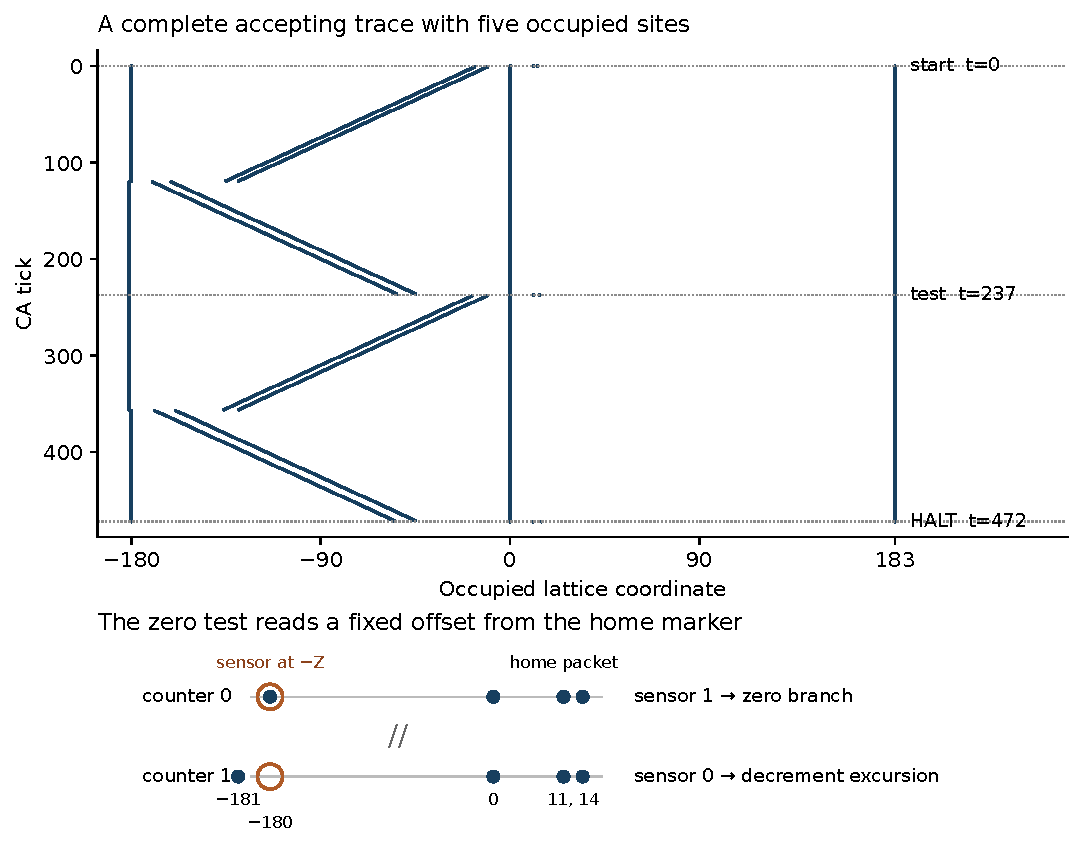
\includegraphics[width=\linewidth]{figures/14-five-binary-five-particle-trace.pdf}
\caption{Top: every occupied site at every tick of the accepting example.
The two excursion clocks are 237 and 235. Bottom: two valid home configurations
at control test, showing the fixed read site $-Z=-180$ for counter values
zero and one. The home packet occupies 11 and 14 in both. The unchanged right
endpoint at 183 is omitted from the bottom detail, and the broken axis
compresses the remote empty interval. The orange circle marks a read location,
not an additional particle or state.}\label{fpa:bc:fig:trace}
\end{figure}

Order branches as bad ADD, start ADD, test positive SUB, test zero SUB.
The two one-hot selector vectors are $(0,1,0,0)$ and $(0,0,1,0)$, with
postcounters $(1,3)$ and $(0,3)$. In the emitted variable order, the complete
clocked natural witness is
\[
 (0,1,0,0,1,3,\ 0,0,1,0,0,3,\ 472).
\]
The file \texttt{example\_frontend.json} explicitly contains its 12 squared
residual slots, 11 of them nonzero, in 13 variables. It has degree at most
four, 48 collected residual monomial occurrences and expansion bound 288.
The first-layer zero guard specializes to zero since the initial tested
counter is zero, explaining the one empty residual without changing the slot
ledger. The provided witness evaluates the polynomial to zero. An independent
fresh generator reconstructs both this JSON and its witness byte-for-byte,
then separately replays the CA to validate that the polynomial clock is the
actual first halt time.

\subsection{External input variants and their costs}
The universal raw positive-input interface can be parameterized mathematically
by an external natural $x$ using $a_0=x+1,b_0=0$. This is an input coordinate,
not a trace witness. It preserves the variable, degree and uniqueness
statements. However substitution into first-layer zero guards can produce
additional monomial occurrences, for example
$e(x+1)=ex+e$. The atomic-input bound \eqref{fpa:bc:eq:rawcost} must therefore be
recomputed for that emitted substitution; it is not inherited without charge.
This optional symbolic substitution is not implemented by the present
constant-input emitter.

Similarly the loading map $(L,R)\mapsto2^L3^R$ is outside the polynomial
trace compiler. These exponentials are not silently treated as polynomial
atoms inside \eqref{fpa:bc:eq:sos}. The certificate begins with the supplied natural
physical counters and describes exactly $h$ literal source instructions.
The primary TM input, its stack encoding and prime loading remain separate
computable inputs with potentially enormous costs.

\section{Executable specification and independent checks}\label{fpa:bc:sec:checks}
The released compiler \texttt{five\_binary.py} is the executable counterpart
of Sections~\ref{fpa:bc:sec:geometry}--\ref{fpa:bc:sec:counts}; \texttt{frontend.py} emits
the residuals in Sections~\ref{fpa:bc:sec:frontend}--\ref{fpa:bc:sec:real}. Their final
SHA-256 digests are recorded in the release manifest and audit receipts:
\begin{quote}\small\ttfamily
five\_binary.py\\
\seqsplit{9022006a4669c7c637ac337a89ea792c55612c23a92c7bedda34af9c9707d90f}\\[4pt]
frontend.py\\
\seqsplit{4d5b3ce9facb439d60a152890b3910c021b242996fbecbeefef7e4c0ba793ca5}\\[4pt]
source-replay/source/literal2.json\\
\seqsplit{85e16b44828f2f3d4ad6d0805dcc9e9922893a6d286874f2018d6a33af864b00}
\end{quote}
The final API hardening changes neither the valid mathematical rule nor the
small and universal polynomial fixture bytes. Source rows are copied into
immutable snapshots; machine, CA and frontend lookup data cannot be changed
after construction. Mutating the caller's original dictionary or lists does
not mutate the compiled rule.

Public source counters and horizons require exact nonnegative Python integers,
including on halt fast paths; Boolean and floating-point substitutes are
rejected. Occupied-site coordinates are exact integers, with negative integers
allowed. Duplicates in a supplied coordinate iterable, Boolean coordinates and
floating-point coordinates are rejected before converting to a set. Source
instruction lengths, operations, counters and destinations are validated.
These are host-language representation contracts. They must be distinguished
from malformed \emph{binary configurations}, whose distinct integer occupied
sites are legitimate inputs to the CA and whose conservation was proved
without an encoding promise.

The natural witness evaluator uses exact natural integers. The paid real
version's numerical sample evaluator accepts nonnegative integers and exact
\texttt{Fraction} values, rejecting floats, NaN and infinities. The exported
polynomial has the proved real-orthant semantics over all nonnegative reals;
this exact sample evaluator is not a claim to implement arbitrary real
arithmetic.

The evidence has four logically separate layers:
\begin{enumerate}
\item The mathematical component proof establishes arbitrary-configuration
conservation, finite locality and all-natural-input simulation.
\item The source proof establishes the all-input TM-to-three-counter and
three-to-two-counter simulation; the primary-source review establishes the
finite-input universal machine and exact table interpretation.
\item Independently written finite tests challenge boundary geometry, local
central outputs, conservation, exact clocks, observer exclusivity and witness
fibers. They provide falsifiable regression evidence, not a replacement for
unbounded proofs.
\item Fresh extracted replay verifies portable operation and byte identity of
code, source, examples and report fixtures against the manifests.
\end{enumerate}

The independent compiler audit covers 450 complete source macros, 52,885
analytical microstates, 238,835 local-center comparisons, 9,907 finite
conservation cases and 9,520 translation comparisons. It also includes 1,190
pair/triple shapes with sensor variants, 4,096 exhaustive dense words, 51 long
connected boundary phases, 1,000 adversarial multiple-component cases and
288 periodic words. Separate literal-source boundary replay covers every one
of the 8,408 controls, 16,816 zero/one counter cases and 205,004 transitions
at dispatch, separation, target contact, reversal and home commit.

The frontend audit checks 2,016 fixed-input instances, 27,504 one-hot branch
sequences, 888 rational-coordinate mutations and 4,998 rational simplex points.
It checks the unpaid fractional counterexample and the paid correction.
The normal and optimized API suites each reject 904 invalid calls and survive
24 mutation/deletion attempts, including caller snapshot isolation. The full
independent mathematical regression suites run against both ordinary and
actual Python \texttt{-O} compiler imports. In the optimized runs, the audit
entry points are compiled with assertions explicitly retained; an optimized
interpreter therefore cannot make the audit pass by discarding its checks.

The producer also records 252 source macro cases, 186,386 CA microsteps,
428 multi-instruction source steps, 1,200 malformed finite configurations,
24,769 local-site checks and 20 local boundary cases. These ledgers are
reproducible counts of executed checks. None is a machine-checked theorem
about all source programs or all binary neighborhoods.

\subsection{Portable replay and artifact identity}
The top-level \texttt{replay.py} requires only Python 3.10 or later and its
standard library. It verifies all manifest hashes, runs the source verifier,
producer checks, independent normal and optimized suites, API checks, and
report-fixture reconstruction, and then verifies unchanged manifest bytes
again. It also tests the mathematical values printed in this report against
the exact fixture JSON. The release verification receipt records the fresh
archive extraction and replay result. No network or package installation is
needed for replay.

The PDF was built from the accompanying LaTeX and all pages were rendered
and visually inspected. Rebuilding the main document requires a conventional
LaTeX installation with the listed packages and the supplied vector figure.
Re-rendering the optional figure requires matplotlib; figure regeneration is
not a dependency of the standard-library verification. The vector graphic,
its source and the exact 473-state trace data are all included and hashed.
The companion Report 12 files are byte-preserved and independently hashed,
not regenerated as part of the new replay.

\wtag\ Neither the companion Report~12 files nor the delivered PDF are shipped with this report; the replay files are shipped under the prefix \path{14-five-binary-}, and three heavy generated inputs of the replay (\texttt{universal\_h1\_frontend.json} and the two \texttt{literal2} files) are rebuilt as described in the README.

\section{Further research directions}\label{fpa:rep:14:last}\label{fpa:bc:sec:questions}
The following are useful directions suggested by the construction. They are
not assertions that no prior work addresses them.
\begin{enumerate}
\item \textbf{Reduce the geometric constants.} The buffer inequalities are
intentionally generous. A smaller $K$ or a tighter locality proof could reduce
radius and observer length. A change must preserve malformed-input conservation,
not only valid trajectories, and must re-check every contact phase.
\item \textbf{Compress control without extra particles.} The present packet
gap alphabet has $m+2p$ codes. Determine which control and phase distinctions
can be merged without ambiguous travel direction, incorrect zero branches
or a premature halt code.
\item \textbf{Obtain alternative literal universal sources.} Fewer ADD/SUB
controls directly reduce $D$, $R$, the indexed schema count and polynomial
branch count. Any replacement needs its own finite-input interface, all-input
proof and complete pinned literal table; row count is not a universality test.
\wtag\ Report~16 (Part~\ref{fpa:part:two}) supplies another literal universal source with a complete pinned table and all-input proof, reversible but much larger (122,622 controls, 141,561 rows), for Report~15's reversible compiler; it does not reduce the constants of this construction.

\item \textbf{Formalize the full-shift extension.} A proof-assistant development
could link component parsing, disjoint bounded-write hulls and the local Boolean
evaluator, then verify the all-input simulation invariant and exact clock.
This would close the current gap between mathematical audit and formal proof.
\item \textbf{Account for bit complexity end to end.} The current report charges
numeric counter height, physical time, spatial extent and algebraic occurrences.
A full bit-cost analysis should include stack loading, prime encoding,
arbitrary-precision arithmetic, source expansion and polynomial serialization.
\item \textbf{Separate finite-horizon from unbounded arithmetic.} The explicit
unique-witness family does not combine its unbounded horizon into one fixed
polynomial. Investigate what additional machinery would achieve such a theorem,
without treating a family of ever-larger tableaux as a fixed-arity result.
\item \textbf{Study other particle models and observations.} Several unit
labels, active zero-weight backgrounds, reversible restrictions and intrinsic
universality alter the assumptions behind the lower or upper bounds. Their
thresholds require separate arguments.
\item \textbf{Complete the primary literature comparison.} Obtain missing full
papers and later primary work before making any novelty, priority or
optimal-resource claim. The construction's internal correctness does not answer
that historical question.
\end{enumerate}

\fpapart{A literal universal reversible source (Report 16)}{fpa:part:two}

\reportopening{16}{A literal universal reversible two counter source}{Complete expanded transitions and all input proofs for a binary five particle compiler}{Report 16 \quad Mathematical construction and reproducible audit}

\begin{reportabstract}{16}
This report supplies the fully expanded universal source left existential in
Report 15. One pinned machine has 122,622 controls and 141,561 literal
zero-test, positive-test, increment, decrement and identity branches on exactly
two natural counters. Its transition function is a partial injection on all
natural configurations, its start control has no incoming branch, and its halt
control has no outgoing branch. We give the finite-tape loader, complete
unbounded-input invariants and termination ranks for every simulation layer,
and exact state-dependent clocks. The construction starts from the published
Neary--Woods 15-state two-symbol Turing machine and uses directly proved and
independently reconstructed reversible history and prime-arithmetic graphs.
Its clean input family has no premature blocking: nonhalting is equivalent to
infinite continuation. Consequently the fixed binary five-particle compiler
instance also has undecidable positive return and periodicity on this family.
All source rows, reconstruction checks and source-level ledgers are bundled.
The much larger cellular-automaton factor list, local truth table and
universal-instance quartic polynomial are not materialized. Even empty-tape
initialization has a predicted two-counter clock near $8\cdot10^{13}$ steps;
only small literal macros and the fresh entry have been executed. A shared-offset primitive certificate reduces the fixed-horizon core to
$141\,565K$ witnesses and $23\,435K+1$ squares. Exact
certificate counts, reproducibility boundaries, and useful next questions are
included. This is an ordinary mathematical proof with executable audits, not
a proof-assistant formalization, efficient simulation, novelty claim or size
record.
\end{reportabstract}

\wtag\ Delivered as \path{Literal_Universal_Reversible_Source_Package.zip} (batch~82, archive~13; arrival \texttt{db37d18c8}), dated 3~October 2026; files placed by \texttt{bca6383e9} with the prefix given in Appendix~\ref{fpa:app:provenance}. Report~16 materializes the universal source that Report~15 (Part~\ref{fpa:part:one}) left existential. Its main file \texttt{report16.tex} and its ten section files are inlined.

\section{The machine and the exact claim}\label{fpa:rep:16:first}\label{fpa:ls:sec:source}
We use $\N=\{0,1,2,\ldots\}$. An instantaneous description (ID) of a
$k$-counter machine has a control $q\in Q$ and a vector $(c_0,\ldots,c_{k-1})\in\N^k$.
A primitive $(q,i,x,t)$ uses a counter index $i$, source and destination
controls $q,t$, and one of five symbols:
\begin{center}
\begin{tabular}{clll}\toprule
Symbol & Enabling condition & Counter change & Cost\\\midrule
$Z$ & $c_i=0$ & none & 1\\
$P$ & $c_i>0$ & none & 1\\
$+$ & true & $c_i\gets c_i+1$ & 1\\
$-$ & $c_i>0$ & $c_i\gets c_i-1$ & 1\\
$0$ & true & none & 1\\\bottomrule
\end{tabular}
\end{center}
Successful tests are separate steps. A combined conditional decrement is used
only in an earlier irreversible layer and is explicitly split before the
reversible construction. No unbounded register is stored in a control name.

\begin{theorem}[Pinned literal universal source]\label{fpa:ls:thm:literal}
Let $M$ be precisely \code{source/source.json} in this release. It has
122,622 controls and 141,561 branches, two natural counters, and class cutoff
$J=0$. Its one-step relation is an injective partial function on
$Q\times\N^2$. No branch enters $\START$, and no branch leaves $\HALT$.

Let $U$ be the Neary--Woods machine in Table 16 of \cite{fpa:nw}.
For every $L,R,T\in\N$ and every $C\ge1$ with $\gcd(C,2310)=1$, the run of
$M$ from
\[
             (\START,C2^L3^R5^T,0)                         \tag{1}\label{fpa:ls:eq:input}
\]
reaches $\HALT$ if and only if $U$, started in state $A=u_1$, scanning the
blank symbol $0=c$, with finite half tapes represented by $L,R$, reaches its
undefined $J1=(u_{10},b)$ transition. Every such source run either reaches
$\HALT$ in finite time or continues forever. This input family includes an
effective encoding of every program and finite input in the published
universality theorem. Thus this one fixed literal machine is computation
universal.
\end{theorem}
The theorem's proof is the complete layer-by-layer argument below. The table's
SHA-256 is
\begin{center}\small\ttfamily
38c586706fa1069442d3e5103151adb156448\\
b7d7c783f5c46d9d507b87fe73a
\end{center}
The line break is typographical; the digest has 64 hexadecimal characters.
The release manifest pins every other artifact independently.

The unrestricted all-natural statement is \emph{partial injection}; the
universality and no-premature-blocking statements have the clean-input promise
(1). An arbitrary second physical counter is not permitted. Nor may arbitrary
initial powers of 7 and 11 be silently added: these encode history and work
counters in the construction. The advertised loader initializes both to zero.
The history invariant actually permits an arbitrary initial history exponent,
but does not permit arbitrary nonzero work. We retain the narrower clean API.

\subsection{What is literal and what remains a finite specification}
Every operation of $M$ is a row in the saved JSON. The Python generator,
macro certificates, prime list, proofs and checkers are \emph{not} primitives
available to $M$. They explain or verify the finite table. There are no row
callbacks, arithmetic oracles, unexpanded macro invocations, symbolic infinite
lists or hidden work counters in the two-counter source.

By contrast, the downstream binary CA is given by the already audited finite
\emph{indexed construction} of Report 15 applied to this literal source.
Its enormous factor array and truth table have not been allocated. The fixed
source horizon quartic is likewise specified by a counted finite formula;
no giant universal-instance polynomial is included. Distinguishing these
materialization levels prevents the new source artifact from implying work
that was never performed.

\begin{figure}[ht]
\centering
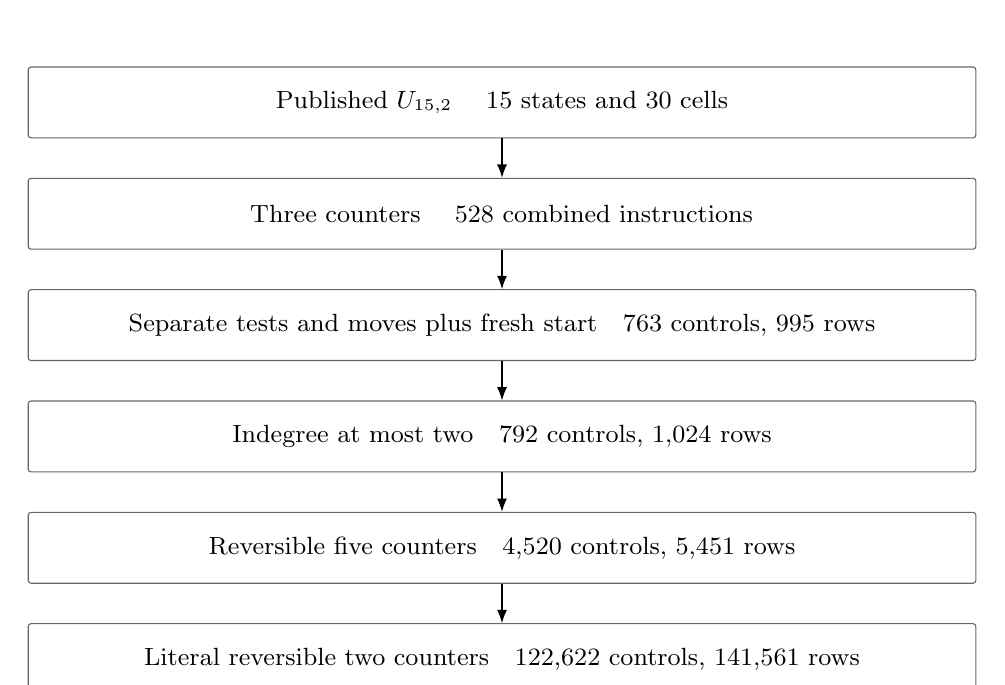
\begin{tikzpicture}[node distance=5mm,>=Latex,
  box/.style={draw=black!60,rounded corners=1pt,align=center,text width=11.8cm,
  minimum height=9mm,font=\small}]
\node[box] (tm) {Published $U_{15,2}$ \quad 15 states and 30 cells};
\node[box,below=of tm] (v) {Three counters \quad 528 combined instructions};
\node[box,below=of v] (s) {Separate tests and moves plus fresh start\quad 763 controls, 995 rows};
\node[box,below=of s] (n) {Indegree at most two\quad 792 controls, 1,024 rows};
\node[box,below=of n] (r) {Reversible five counters\quad 4,520 controls, 5,451 rows};
\node[box,below=of r] (p) {Literal reversible two counters\quad 122,622 controls, 141,561 rows};
\foreach \a/\b in {tm/v,v/s,s/n,n/r,r/p} \draw[->] (\a)--(\b);
\end{tikzpicture}
\caption{All counter-machine stages are saved as finite literal tables. The
last stage, rather than an existence citation, is the input to Report 15.}
\label{fpa:ls:fig:pipeline}
\end{figure}
\section{The finite tape and the irreversible front end}\label{fpa:ls:sec:frontend}
\wtag\ \textbf{A second presentation.} The 528-instruction three-counter front end of this section, with its file \code{virtual3.json}, is byte for byte the program of quadratic-orthant-certificates Part~V (shipped there as \path{data/16-universal-membrane-virtual3.json}); its correctness is that report's Lemma \path{qoc:um:lem:virtual}. It is kept here because the later layers cite its clocks. The prime encoding of Section~\ref{fpa:ls:sec:primes} is a reversible variant of that report's Lemma \path{qoc:um:lem:prime}, not the same lemma.

\subsection{Primary table and exact finite loader}
The 30 cells of Table 16 in \cite{fpa:nw} were compared with the saved
\code{tm\_table.json} against rendered primary PDF page 17 (printed page 121).
Printed page 112 was also visually checked for the input conventions. The
machine table, using $0=c$, $1=b$, and states $A,\ldots,O$ for
$u_1,\ldots,u_{15}$, is reproduced here. An entry writes its first symbol,
moves as specified, and enters its last state.
\begin{center}
\begin{tabular}{c*{5}{c}}\toprule
Scanned & A & B & C & D & E\\\midrule
0 & 0RB & 1RC & 0LG & 0LF & 1RA\\
1 & 1RA & 1RA & 0LE & 1LE & 1LD\\\midrule
Scanned & F & G & H & I & J\\\midrule
0 & 1LD & 0LH & 1LI & 0RA & 1LK\\
1 & 1LD & 1LG & 1LG & 1LJ & undefined\\\midrule
Scanned & K & L & M & N & O\\\midrule
0 & 0RL & 0RM & 0LB & 0LC & 0RN\\
1 & 1RN & 1RL & 1RL & 0RO & 1RN\\\bottomrule
\end{tabular}
\end{center}
The undefined cell is $J1$, not $J0$. A known prose/display discrepancy later
in the article is not a reason to alter the pinned transition table. The
old bibliographic comment in the byte-preserved compact machine file gives
inaccurate page numbers; the bibliography of this report uses the corrected
105--126 range without editing that dependency.

\wtag\ \textbf{Correction (3~October 2026).} Here too the ``old bibliographic comment'' gives the publisher's pages: Neary--Woods is \emph{Fundamenta Informaticae} 91(1) (2009), 123--144, DOI \path{10.3233/FI-2009-0036}; 105--126 is the author-hosted PDF's pagination, and the DOI \path{10.3233/FI-2009-0008} that Report~16 printed belongs to another paper (Appendix~\ref{fpa:app:provenance}). The table above agrees entry by entry with Table~\ref{fpa:bc:tab:tm} and with quadratic-orthant-certificates' Table \path{qoc:wf:tab:tm}, where the $(u_{10},b)$ discrepancy is recorded.

Definition 3.1, equations (3)--(4), Tables 1--3 and Section 3.5 of the primary
paper specify the finite program/data encoding. Its separator $G$ for this
machine is $bc$, and the initial head is on its rightmost symbol $c=0$.
Thus fixing the initially scanned symbol to zero retains the universal input
family. Both tails are blank $c$, rather than nonblank periodic backgrounds.
The reduction from an arbitrary program/input to that finite universal tape
is the published universality dependency, not a claim that the loader below
reimplements the full program compiler.

Place the head at coordinate zero. For finite nearest-head-first words
$\ell=\ell_0\cdots\ell_{a-1}$ and $r=r_0\cdots r_{b-1}$, put symbol
$\ell_i$ at $-i-1$ and $r_i$ at $i+1$. Unmentioned cells and the scanned
cell are zero. Define
\[
 L=\sum_{i<a}\ell_i2^i,\qquad R=\sum_{i<b}r_i2^i,
 \qquad \mathcal L(\ell,r)=(\START,2^L3^R,0).             \tag{2}
\]
\code{loader.py:from\_tape} implements exactly (2). Its checks reject
nonbinary characters and non-string tape arguments. The counter interface
\code{from\_counters} supplies optional $T,C$ from (1), rejecting Boolean
pseudo-integers, negative values, zero cofactors and cofactors not coprime to
2310. These APIs return exact integers. The command-line interface prints
hexadecimal to avoid interpreter decimal-digit limits.

Every input gives finite values by finite sums and powers. This is a
computability statement, not a feasible-memory promise. For example,
\code{left=101,right=01} means $L=5,R=2$ and physical input $A=288,B=0$.
The loader neither simulates $U$ nor solves any halting question.

\subsection{Three counters with the scanned symbol in control}
The pinned three-counter program has 528 active instructions: 295 increments
and 233 combined conditional decrements. It uses data counters $L,R$ and
scratch $T$. A combined instruction $\operatorname{SUB}(i,q,z)$ decrements a
positive $c_i$ and goes to $q$, or leaves zero unchanged and goes to $z$.
An increment is unconditional. Consequently every nonhalt instruction is
enabled on every natural vector.

At a TM cut, the state and scanned bit are in finite control, the two half
tapes use low-order bits nearest the head, and $T=0$. The initial prologue is
\[
 \mathsf{init\_clear\_T}:\quad
 \operatorname{SUB}(T,\mathsf{init\_clear\_T},\mathsf{tm\_A0\_pop0}).
                                                               \tag{3}
\]
It takes exactly $T+1$ combined instructions and clears arbitrary initial
scratch. The later reversible history retains enough information to invert
this clearing; no irreversible erasure is asserted for the final machine.

For a defined TM instruction $(q,s)\mapsto(w,D,q')$, let $X$ be the half
tape in the direction $D$ and $Y$ the other half tape. Write $X=2Q+\rho$,
$\rho\in\{0,1\}$. The following finite graph is instantiated separately for
each instruction and parity branch. Labels denote controls, not procedures
called by the final machine:
\begin{align*}
 \mathsf{pop0}&:\operatorname{SUB}(X,\mathsf{pop1},\mathsf{back0}),\\
 \mathsf{pop1}&:\operatorname{SUB}(X,\mathsf{pair},\mathsf{back1}),\\
 \mathsf{pair}&:\operatorname{ADD}(T,\mathsf{pop0}).
\end{align*}
After $k$ full loops, $X=2(Q-k)+\rho$ and $T=k$. For $k<Q$ both
subtractions are enabled. The rank $Q-k$ decreases. At $k=Q$, one failed test
if $\rho=0$, or one success and a failure if $\rho=1$, determines the bit
$\rho$ and leaves $X=0,T=Q$.

For the selected parity, a transfer loop alternates a successful
$\operatorname{SUB}(T)$ with $\operatorname{ADD}(X)$, then takes the zero exit.
After $j$ transfers $X=j,T=Q-j$; rank $T$ proves termination at $X=Q,T=0$.
The whole pop stage takes
\[
                    3Q+1+\rho+2Q+1=5Q+\rho+2.        \tag{4}
\]

The push loop consumes one $Y$ and adds two units to $T$ per iteration.
After $k$ iterations $Y=Y_{\rm old}-k,T=2k$; rank $Y$ decreases. At exit,
$Y=0,T=2Y_{\rm old}$. A second transfer loop decreases $T$ one at a time and
increases $Y$, preserving $Y+T=2Y_{\rm old}$. This terminates at
$Y=2Y_{\rm old},T=0$. If $w=1$, one final increment writes the new low bit;
if $w=0$, the control edge is linked directly to the next cut. The next state
is $(q',\rho)$. The push cost is $7Y_{\rm old}+2+w$. Hence one TM step costs
exactly
\[
             5Q+\rho+7Y_{\rm old}+w+4                  \tag{5}\label{fpa:ls:eq:tmclock}
\]
combined instructions and realizes
$(X,Y,T)\mapsto(Q,2Y_{\rm old}+w,0)$, exactly the TM update.

All 29 defined TM cells use this graph. The undefined $J1$ continuation is
$\HALT$ and has no instruction. The loops have no internal halt and terminate
for every natural half tape by the displayed ranks. A cut requires both its
control label and $T=0$: the pop loop can revisit its entry label with $T>0$.
Checking labels alone would give a false simulation boundary. The saved-row
checker covers all 528 instructions with 437 affine paths, using arbitrary
natural parameters rather than a finite sample grid.

\subsection{Separate tests and a genuinely fresh start}
Replace every combined $\operatorname{SUB}(i,q,z)$ by a zero test to $z$,
and a positive test to a fresh private control followed by a decrement to
$q$. The zero case takes one primitive step; the positive case takes two.
An original increment still takes one. If a virtual trace uses $v$ combined
instructions with $v_+$ successful conditional decrements, its split cost is
$v+v_+$.

The old initial control in (3) has a self-loop and cannot be declared
predecessor-free. Insert $\START$ with one identity edge to that control
\emph{before} reversibilization. This changes no data and costs one step.
The literal split table has 763 controls and 995 rows. Its start has no
incoming row and halt has no outgoing row. No reversible edge is casually
prepended at a later stage, where it could create an overlapping range.

\subsection{Reducing indegree without changing data}
For an original target with ordered incoming rows $e_1,\ldots,e_k$, $k>2$,
introduce $k-2$ private merge controls $u_1,\ldots,u_{k-2}$. Redirect $e_1,e_2$
to $u_1$, and $e_j$ to $u_{j-1}$ for $3\le j<k$, leaving $e_k$ directed to
the old target. Chain the new controls by identity rows toward that target.
Every new merge has indegree two, and the old target receives only the chain's
last edge and $e_k$. No operation is changed.

The extra cost after row $e_j$ is
\[
                         k-\max(2,j).                  \tag{6}
\]
The number of remaining chain nodes is a strictly decreasing rank; all chains
are finite and cannot block. The present table has 16 affected targets, adding
29 controls and 29 identity rows. The normalized source has 792 controls and
1,024 rows. Edges into halt are normalized too. The no-incoming start and
no-outgoing halt conditions survive unchanged.
\section{Reversible history with five counters}\label{fpa:ls:sec:history}
\wtag\ Sections~\ref{fpa:ls:sec:history}--\ref{fpa:ls:sec:composition} make literal the existence argument of signal-machine-collision-certificates Part~IV, \S\path{smc:sl:sec:safe} (Morita's history counter, a scratch counter, prime encoding with a scratch-zero invariant, and induction on legal progress): here the machine is fixed and its costs and termination ranks are exact. In substance this answers that report's question ``Print one safe universal source'' (Part~IV, \S\path{smc:sl:sec:questions}, item~1), for the guarded syntax of Report~15 rather than source~13's pulse interface.

The construction is inspired by Morita's separate-test and separate-move
machines \cite{fpa:morita1996}, in particular the history and counter-reduction
constructions. Primary text extraction was consulted at printed pages
308--309 and 314--316. The scan could not be visually verified: PDF screenshot
requests failed and a live download endpoint returned HTML. We therefore
make no visual-transcription claim for Morita's diagrams or ambiguous OCR.
Instead the actual local graphs below are explicitly generated, independently
reconstructed from their preceding layer, and proved directly. No uncertain
OCR symbol is a premise of the proof.

Add history $H$ and work $W$ to the normalized three-counter source. Its
boundary invariant is
\[
                   (\mathbf d,H,W)=(\mathbf d,h,0),\quad h\in\N, \tag{7}
\]
where $\mathbf d=(L,R,T)$. At a target with fewer than two incoming edges,
or with a complementary $Z/P$ pair on the same counter, leave the incoming
rows unchanged. Those images are already disjoint. Such a row costs one step
and leaves $H,W$ unchanged.

Every other indegree-two target has a colliding pair. Give its rows branch
numbers $b=0,1$. Each new path first executes its original source operation,
then checks $W=0$ and enters a history transfer loop. In particular, a
negative update is blocked before history work when its original counter is
zero. The source guard has not been weakened.

\begin{lemma}[Exact history macro]\label{fpa:ls:lem:history}
For every enabled colliding source row and every $h\ge0$, its expanded path
maps $(\mathbf d,h,0)$ to $(\mathbf d',2h+b,0)$ at the old destination in
exactly $10h+4+2b$ primitive steps. It cannot stop or run forever internally.
\end{lemma}
\begin{proof}
After the source operation and work-zero guard, the transfer loop has
\[
                   H=h-j,\quad W=j,\quad 0\le j\le h.   \tag{8}
\]
One iteration tests $H>0$, decrements $H$, increments $W$, and tests $W>0$.
It costs four steps. Rank $H$ decreases, and every decrement has its required
positive test. At the final $H=0$ test, the pair is $(0,h)$.

Branch zero enters the doubling loop directly. Branch one first increments
$H$ and tests $H>0$, taking two steps. At the doubling-loop test after $j$
iterations, the invariant is
\[
                   H=b+2j,\quad W=h-j,\quad 0\le j\le h.\tag{9}
\]
One iteration tests $W>0$, decrements $W$, increments $H$, tests $H>0$,
increments $H$ again and tests $H>0$ again. It costs six steps and decreases
rank $W$. The final zero test on $W$ reaches the original destination with
$(2h+b,0)$. All post-increment positive tests are enabled. The exact cost is
\[
            1+1+4h+1+2b+6h+1=10h+4+2b.                \tag{10}
\]
Both ranks and all guards remain valid when $h=0$: the two branches cost four
and six steps respectively.
\end{proof}

\begin{figure}[ht]
\centering
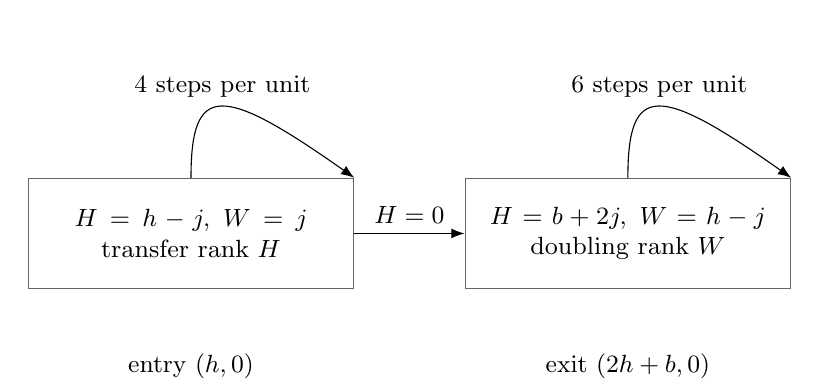
\begin{tikzpicture}[>=Latex,node distance=10mm,
 n/.style={draw=black!60,align=center,text width=3.9cm,minimum height=14mm,font=\small}]
\node[n] (a) {$H=h-j,\ W=j$\\transfer rank $H$};
\node[n,right=14mm of a] (b) {$H=b+2j,\ W=h-j$\\doubling rank $W$};
\draw[->] (a)--node[above,font=\small] {$H=0$} (b);
\draw[->] (a.north) .. controls +(0,12mm) and +(-17mm,12mm) .. node[above,font=\small] {4 steps per unit} (a.north east);
\draw[->] (b.north) .. controls +(0,12mm) and +(-17mm,12mm) .. node[above,font=\small] {6 steps per unit} (b.north east);
\node[below=7mm of a,font=\small] {entry $(h,0)$};
\node[below=7mm of b,font=\small] {exit $(2h+b,0)$};
\end{tikzpicture}
\caption{The two history invariants. Branch one pays two additional steps
between the loops. This diagram summarizes the fully expanded finite graph;
it is not an extra machine operation.}
\label{fpa:ls:fig:history}
\end{figure}

\subsection{Why history recording is globally reversible}
The guards inside this graph do more than ensure intended execution. At a
transfer-loop entry, its first arrival has $W=0$, while loop returns have
$W>0$. At the joins in the doubling part, the relevant incoming paths have
$H=0$ and $H>0$. These are disjoint image conditions on all natural inputs.
Replacing the displayed tests by identity arrows would destroy reversibility.

More generally, the independent graph checker groups all rows by source
control and all rows by destination control. Any group with more than one row
must be exactly a complementary $Z/P$ pair on the same counter. Each single
primitive is an injective partial map; those pairs have disjoint domains
when outgoing and disjoint images when incoming. Therefore the \emph{entire}
five-counter relation is deterministic and partial-injective, including on
unclean work values or unreachable configurations. This is a finite structural
proof of an all-natural property, not a test of sample histories.

There are 233 recording pairs, hence 466 replaced incoming rows. Each pair's
explicit graph uses 21 rows in place of its two and adds 16 controls. Thus
\[
 1024+233(21-2)=5451,\qquad 792+233\cdot16=4520.          \tag{11}
\]
The actual row multiset is compared with an independently reconstructed graph;
the count is not used as a substitute for that comparison. Private controls
are fresh and no source destination is entered before the macro terminates.
All normalization edges, including those into halt, were included in this
history pass.
\section{Prime encoding into exactly two counters}\label{fpa:ls:sec:primes}
Use primes $(p_0,p_1,p_2,p_3,p_4)=(2,3,5,7,11)$. At a five-counter
boundary, represent $\mathbf a=(a_0,\ldots,a_4)$ by
\[
 A=C\prod_{i=0}^4p_i^{a_i},\qquad B=0,
 \qquad C\ge1,\quad\gcd(C,2310)=1.                    \tag{12}\label{fpa:ls:eq:prime}
\]
Unique factorization says $a_i>0$ exactly when $p_i$ divides $A$; it says
$a_i=0$ exactly when $p_i$ does not divide $A$. The cofactor $C$ is preserved.
Although $A$ can vanish inside a macro, it is positive at every boundary.
At the initial boundary, $a_3=a_4=0$, giving (1).

One identity source edge is copied as one physical identity edge. For all
other source edges, a zero test first checks $B=0$. The remainder below is
always a bounded finite-control index from $0$ to $p-1$, not an uncounted
natural register. The construction has 4,519 source macros, one for each
nonterminal five-counter source control, and 2,330 destination-shared
restorers. Complementary source tests at one control share one division
macro. All graphs are expanded in the saved two-counter table.

\subsection{Common transfer for arithmetic moves}
For a prime $p$ and boundary value $A=N\ge1,B=0$, both the multiplication
and division graphs first transfer $A$ to $B$. At the loop test after $j$
iterations,
\[
                       A=N-j,\quad B=j,\quad0\le j\le N.\tag{13}
\]
An iteration tests $A>0$, decrements $A$, increments $B$, then tests $B>0$.
It costs four steps and decreases rank $A$. The final $A=0$ test produces
$(0,N)$. Including the initial $B=0$ guard, this phase costs $4N+2$.
The post-increment positive guard is important to the all-natural reverse
join, even though it is automatic on the intended forward path.

\subsection{Multiplication and an encoded increment}
At the multiplication-loop test after $j$ iterations,
\[
                        A=pj,\quad B=N-j,\quad0\le j\le N.\tag{14}
\]
One iteration tests $B>0$, decrements $B$, performs exactly $p$ increments
of $A$, then tests $A>0$. It costs $p+3$. Rank $B$ decreases and the final
$B=0$ test reaches the five-counter target encoded as $(pN,0)$. The full
clock is
\[
                  4N+2+(p+3)N+1=(p+7)N+3.             \tag{15}
\]
Every decrement is enabled and every positive post-increment test is valid;
there is no internal blocking on a promised input. Multiplying by $p_i$
increments just the corresponding encoded exponent.

\subsection{Division and an encoded decrement}
For an enabled source decrement, $N=pQ$ with $Q\ge1$. After the common
transfer, the division-loop invariant after $j$ groups is
\[
                     A=j,\quad B=p(Q-j),\quad0\le j\le Q.\tag{16}
\]
A group tests $B>0$, makes exactly $p$ decrements of $B$, increments $A$,
and tests $A>0$. It costs $p+3$. Since $B$ is a positive multiple of $p$
at each continuing test, all $p$ decrements are enabled. The rank $Q-j$
decreases. The final zero test returns $(Q,0)$, with exact total cost
\[
                  4N+(p+3)Q+3=(5p+3)Q+3.              \tag{17}
\]
This decreases precisely the chosen exponent. On an unpromised
$N=pQ+\rho$, $0<\rho<p$, the graph makes $Q$ full groups, consumes the
remaining $\rho$ units, and blocks at a forced decrement before a source
boundary. Successful termination is not claimed on this disabled case.
In particular it does not falsely reach halt. Global partial injection of
these malformed runs is a separate structural property proved below.

\subsection{Division with a bounded remainder for tests}
A test source control has either one $Z$ or $P$ row, or a complementary pair
on one counter. Let $N=pQ+\rho$, $0\le\rho<p$. At division control $j$
after $k$ complete groups, the invariant is
\[
              A=N-pk-j,\qquad B=k,\qquad0\le j<p,       \tag{18}
\]
whenever the right side is nonnegative. Each consumed unit of $A$ requires a
positive test and decrement, taking two steps. Every full group closes with
an increment of $B$ and a positive test on $B$, adding two steps. The
unconsumed $A$ strictly decreases between at most two group-close steps.
Thus no infinite run is possible in the division phase. Equivalently one may
use a lexicographic rank consisting of unconsumed units and a finite pending
phase index.

The first zero test on $A$ occurs at remainder control $\rho$, with
$A=0,B=Q$. The clock through that zero test, including the entry guard, is
\[
                            2N+2Q+2.                  \tag{19}
\]
Remainder zero means the encoded counter was positive and selects its $P$
destination. Remainders $1,\ldots,p-1$ mean it was zero and select its $Z$
destination. If the source has only one of these tests, the other exit is
absent. A false singleton test blocks in this division graph and never enters
a source boundary. For an enabled source test, the correct exit exists.

\subsection{Destination sharing is essential for restoration}
For the selected target, enter its \emph{shared} restorer at remainder index
$\rho$. First add $\rho$ to $A$, using an increment and positive test for
each unit. At remainder-zero control the pair is $(\rho,Q)$. After $j$
whole restoration groups,
\[
                      A=\rho+pj,\quad B=Q-j,\quad0\le j\le Q.\tag{20}
\]
A group consists of a positive test and decrement on $B$, then $p$ pairs of
increment and positive test on $A$. Its cost is $2p+2$ and rank $B$
decreases. The last zero test returns $(N,0)$ to the chosen five-counter
destination. Restoration costs
\[
                           2\rho+(2p+2)Q+1.           \tag{21}
\]
Combining (19) and (21) and using $N=pQ+\rho$ gives the exact test clock
\[
                   4N+4\lfloor N/p\rfloor+3.          \tag{22}
\]
Tests preserve the entire exponent vector and cofactor.

It would be incorrect to build independent restorers per incoming test edge:
two copies would finish with overlapping $B=0$ images at a common source
destination. Instead restoration is shared by destination. Global
reversibility of the five-counter graph ensures that tests entering one
such destination use the same source counter and have at most one zero and
one positive row. The distinct remainder paths enter the shared graph through
complementary zero/positive guards. The independent reconstruction checks
those exact joins and every restorer's prime and target.

\begin{lemma}[Prime macro correctness and exact costs]\label{fpa:ls:lem:prime}
Every enabled five-counter row on a boundary (12) has a unique finite
physical path to its correct encoded destination. No other five-counter
boundary is visited internally. With selected prime $p$ and pre-step encoded
integer $N$, its cost is
\begin{center}
\begin{tabular}{ll}\toprule
Source operation & Physical primitive steps\\\midrule
identity & $1$\\
increment & $(p+7)N+3$\\
enabled decrement & $4N+(p+3)(N/p)+3$\\
enabled zero or positive test & $4N+4\lfloor N/p\rfloor+3$\\\bottomrule
\end{tabular}
\end{center}
Every cost is a finite positive integer. The cofactor remains unchanged.
\end{lemma}
\begin{proof}
The preceding invariants prove the stated postconditions and exact clocks.
Their ranks prove termination, and the positivity arguments prove that no
required decrement or test blocks. All macro-internal controls and restorer
controls are fresh relative to the five-counter boundary controls. The final
edge alone reaches the intended source destination. Unique factorization
translates multiplication, division and remainder tests into exactly the
chosen exponent operation.
\end{proof}

\subsection{Partial injection on every pair and strict serialization}
The two-counter graph satisfies the same structural criterion as the
five-counter graph: any multiple outgoing or incoming group consists of
complementary $Z/P$ tests on one and the same counter. Thus primitive
domains and images are pairwise disjoint on every natural pair. Every
single primitive is individually injective. This proves global partial
injection without a well-formedness promise.

The strict serialized schema maps counter index zero to side $-1$, index
one to side $+1$, updates to $-1,0,+1$, and guards as follows:
\begin{center}
\begin{tabular}{lll}\toprule
Primitive & Serialized domain & Exact image condition\\\midrule
$+$ & true & selected counter $>0$\\
$-$ & selected counter $>0$ & true\\
$Z$ & selected counter $=0$ & selected counter $=0$\\
$P$ & selected counter $>0$ & selected counter $>0$\\
$0$ & true & true\\\bottomrule
\end{tabular}
\end{center}
All other counters are unchanged. Hence domain and image predicates are
constant on each of the four cells formed by $\{0,>0\}^2$; $J=0$ suffices.
The indexed validator derives each image from its original update and guard,
including nonnegativity of the predecessor. It does not trust a separately
supplied image predicate. It checks exact field names and types, valid
references, unique branch names, the guard syntax, natural outputs, source
and target class disjointness, no incoming start and no outgoing halt.
Its four-cell proof covers all natural pairs, rather than only four tested
sample values, because each predicate is constant on those cells.

The final table has 33,436 increments, 32,630 decrements, 23,429 zero tests,
52,036 positive tests and 30 identities. Their sum is 141,561. Thus the
compiler moving and zero-update row counts are
\[
                   p=66\,066,\qquad a=75\,495.          \tag{23}
\]
Certificates specify private-state names, but independent reconstruction
checks their claimed source rows, targets, primes, kinds and coverage before
comparing complete edge multisets. Certificates are not trusted assertions
that an unchecked macro worked.
\section{Composition on all promised inputs and exact clocks}\label{fpa:ls:sec:composition}
\subsection{Finite prefixes and the no blocking theorem}
At an intended boundary, each simulation layer agrees with the preceding
layer on data and control. Section~\ref{fpa:ls:sec:frontend} proves the exact TM
transition for arbitrary natural half tapes and clears arbitrary initial
scratch. Splitting preserves each branch with one or two primitive steps.
Normalization follows it by its finite identity chain. The history layer
preserves the three data counters and updates only $(H,W)$ as in
Lemma~\ref{fpa:ls:lem:history}. The prime layer preserves the representation (12)
and realizes each five-counter primitive by Lemma~\ref{fpa:ls:lem:prime}.

Initialize $(L,R,T,H,W)$ to $(L,R,T,0,0)$. For every finite valid source
prefix, induction on its transitions shows that the literal simulation
reaches the corresponding encoded boundary after the sum of the finite
positive macro costs, with the stated invariants. Fresh internal controls
prevent an unintended layer boundary from being mistaken for the final
state. In the three-counter front end the additional $T=0$ cut condition is
used wherever the loop revisits its entry label. All edges into halt are
included in every expansion; no premature internal halt is available.

\begin{proposition}[Clean runs cannot block before halt]\label{fpa:ls:prop:continue}
On every input (1), either $M$ first reaches $\HALT$ in finite time or its
literal primitive run is infinite. The second case occurs exactly when $U$
does not halt on the associated finite tape.
\end{proposition}
\begin{proof}
The scratch prologue terminates by decreasing $T$. Every nonhalt combined
three-counter instruction is enabled on every natural vector. Every defined
TM step expands into a finite terminating front-end macro. Every enabled
split/normalized edge expands to a finite enabled history macro on $W=0$;
every resulting five-counter edge expands to a finite enabled prime macro
on (12). Thus a valid boundary cannot lead to nonfinal blocking or an
infinite internal stutter. A finite TM halting path reaches literal halt by
composition. If $U$ never halts, it has infinitely many defined steps, and
therefore infinitely many literal steps, since every expanded duration is
positive. Conversely a literal halt must occur at the correctly simulated
halt boundary. This proves both alternatives and completes
Theorem~\ref{fpa:ls:thm:literal}.
\end{proof}
The proposition is stronger than halting equivalence alone. An arbitrary
guarded source could have a finite nonhalt stuck run, which still reflects
periodically under Report 15. Such an input is ruled out here only on the
clean family (1). It is not ruled out for every malformed pair in $\N^2$.

\subsection{The complete clock composition}
There is no claimed uniform constant slowdown. Use the actual intermediate
values to compute the following exact clock layers:
\begin{enumerate}
\item The initial scratch prologue takes $T+1$ combined instructions; each
TM step takes (5) with its own $Q,\rho,Y_{\rm old},w$.
\item Add one fresh-entry step. Charge one for each increment or zero
conditional-decrement branch, and two for each positive
conditional-decrement branch.
\item For each primitive edge $e_j$ entering a normalized indegree-$k$
target, append the $k-\max(2,j)$ identity steps in (6). Unchanged targets
append zero.
\item Let $h_s$ be the pre-step history of each normalized edge. An unchanged
edge has cost one and $h_{s+1}=h_s$. A recording edge of branch $b_s$ has
cost $10h_s+4+2b_s$ and $h_{s+1}=2h_s+b_s$.
\item For \emph{every} resulting five-counter primitive, including history
and work operations, form its actual encoded pre-step integer $N_t$ from
(12), choose its counter's prime, and sum the costs in Lemma~\ref{fpa:ls:lem:prime}.
This gives the exact two-counter primitive time.
\item For every literal two-counter row of the resulting run, use the
Report 15 CA clock in Section~\ref{fpa:ls:sec:binary}. This last sum is the exact
physical CA observation time. One CA step means its entire fixed factor
composition, not one individual local involution.
\end{enumerate}
Each item is a finite sum for any finite source prefix. The formulas are
exact even when calculating the integer or traversing the corresponding
run is impractical. Simulation-prefix induction, rather than empirical
extrapolation, establishes the clock equality.

\subsection{Predicted clocks and what was actually executed}
For the empty finite tape and standard cofactor, the five-counter prologue
from fresh start to the first $A0$ TM cut takes 142 steps and reaches
\[
                         (L,R,T,H,W)=(0,0,0,15,0).
\]
The exact theorem-derived two-counter cost is
\[
                              79\,936\,151\,060\,302.   \tag{24}
\]
The saved clock calculation executes the short five-counter trace and sums
the prime macro formulas. It does \emph{not} traverse these approximately
$8\cdot10^{13}$ two-counter steps. A literal trial was stopped at a
5,000,000-step budget; neither a complete two-counter prologue nor a
universal computation is reported as executed.

\begin{center}
\begin{tabular}{rr}\toprule
$(L,R,T,C)$ & Predicted two-counter prologue clock\\\midrule
$(0,0,0,1)$ & $79\,936\,151\,060\,302$\\
$(1,0,0,1)$ & $159\,872\,302\,120\,216$\\
$(0,1,0,1)$ & $239\,808\,453\,180\,106$\\
$(0,0,0,13)$ & $1\,039\,169\,963\,779\,214$\\\bottomrule
\end{tabular}
\end{center}
These four cases each have the same 142-step five-counter prologue. Initial
scratch $T=1$, even with $L=R=0,C=1$, produces a 459-step five-counter
prologue with $H=47$, and a predicted physical cost exceeding $8\cdot10^{40}$.
The exact full integer is recorded in \code{prologue-predicted-clocks.json}.
This growth is a concrete reason to separate proof-level simulation from
feasible end-to-end testing.

Small macros, history examples and five fresh-entry paths are literally
executed by supplementary tests. The independent macro audit checks 2,330
history traces and 27,743 prime traces. These tests help catch implementation
mistakes; neither their finite ranges nor their runtime budgets establish
universality. The all-input proof comes from complete graph reconstruction,
affine identities, invariants and decreasing ranks.
\section{The fixed binary five particle instance}\label{fpa:ls:sec:binary}
Report 15 supplies the independently audited compiler theorem and its explicit
finite indexed gate construction \cite{fpa:r15}. Its source hypothesis is a
finite two-natural-counter partial injection with terminal halt and guards
constant on finitely many natural-number classes. The present literal source
satisfies those hypotheses on \emph{all} natural IDs by
Section~\ref{fpa:ls:sec:primes}. The source's clean-input restriction concerns
simulation correctness, and does not weaken the compiler's global
reversibility hypothesis.

The exact byte-preserved compiler proof and authored Report 15 are bundled.
Their assertions that their own universal source was not materialized remain
correct descriptions of that earlier release. This report provides the new
source input separately, without silently editing their history or replacing
their finite nonuniversal examples.

\subsection{Indexed construction and global reversibility}
For context, the compiler assigns an unsigned home mode $\HH_q$ to every
source control and two traveling modes to every moving branch. Every mode
has plus and minus versions with distinct gaps in $\{1,\ldots,D\}$. A
head is a close pair of ones whose gap stores one signed mode. Three isolated
ones encode left counter endpoint, origin and right counter endpoint. The
initial five-particle support for source ID $(q,c_0,c_1)$ is
\[
 \enc(q,c_0,c_1)^+=
 \{-(Z+c_0),0,Z+c_1,S,S+d(\HH_q^+)\}.                 \tag{25}\label{fpa:ls:eq:caenc}
\]
There are no other nonzero cells, no extra tracks and no varying background.

Each compiler factor is an isolated equal-mass pattern swap. At an eligible
key it interchanges two finite supports of the same cardinality that are not
translates. Eligibility checks a bounded empty halo, separation from other
raw keys, and, when needed, a context predicate identical at the paired
endpoints. The isolation lemma proves that the \emph{entire raw-key set} and
eligibility are unchanged by the simultaneous rewrite on arbitrary dense or
infinite binary inputs. Applying the same factor again restores the input.
Each factor is therefore a translation-equivariant local involution and
preserves finite numerical mass. A finite composition is globally bijective
on the full binary shift; this conclusion does not rely on admissible-input
simulation or finite-support injectivity.

On encoded inputs the compiler builds a partial-injective micrograph by
subdividing every source move into dispatch, outbound travel, endpoint
update, return travel and commit. A zero-update row is one guarded home edge.
Intermediate modes carry the original branch identity; domains and exact
image predicates make the relevant home joins disjoint. The admissible
intermediate states are precisely the subdivisions of \emph{enabled} source
edges, not every geometrically plausible traveling packet.

A block $E$ swaps the plus end of each microedge with its minus destination.
A block $P$ flips the signed mode. On the admissible doubled graph their
factor products realize those matchings. One CA step is $F=P\circ E$.
Thus a plus state with successor advances one microedge; a minus state with
predecessor moves backward one edge. At a missing edge the sign flips in
one step. The global proof is factor-by-factor even on malformed inputs;
the matching proof is a separate argument only on the precisely defined
admissible set. Report 15 supplies all patterns, contexts and boundary cases.

\subsection{All compiler parameters for this source}
The defining formulas and their exact values are
\begin{center}
\begin{tabular}{llr}\toprule
Parameter & Definition & Value\\\midrule
$m$ & source controls & $122\,622$\\
$p$ & moving rows & $66\,066$\\
$a$ & zero-update rows & $75\,495$\\
$J$ & natural class cutoff & $0$\\
$D$ & $2m+4p$ & $509\,508$\\
$S$ & $2D+2$ & $1\,019\,018$\\
$B_2$ & $D+1$ & $509\,509$\\
$L_{\rm gate}$ & $3D+4$ & $1\,528\,528$\\
$B_3$ & $4D+5$ & $2\,038\,037$\\
$Z$ & $10B_3+10+2J$ & $20\,380\,380$\\\bottomrule
\end{tabular}
\end{center}
The notation $L_{\rm gate}$ distinguishes the compiler isolation constant
from the left half-tape integer $L$. It is called simply \code{L} in the
machine-readable ledger. The factor families are
\begin{align*}
 n_2&=4p=264\,264,\\
 n_3&=8pD+23p+m=269\,290\,886\,364,\\
 n_c&=2p+a=207\,627.
\end{align*}
Therefore the exact indexed factor count and the unoptimized compositional
radius upper bound are
\begin{align}
 N_{\rm factors}&=8pD+29p+m+a=269\,291\,358\,255,       \tag{26}\\
 R_{\rm CA}&=n_2(6D+8)+n_3(24D+32)+n_c(Z+J+12D+16)\notag\\
            &=3\,292\,955\,588\,459\,274\,804.         \tag{27}
\end{align}
This is a radius bound, not a claim of least possible radius. The finite
local binary truth table could in principle be generated by this indexed
composition and would have $2^{2R_{\rm CA}+1}$ slots at the stated radius.
It was not generated. Neither was the list of 269 billion factor objects.

\code{target-ledger.json} and the loader derive these numbers directly from
the pinned source. The original eager \code{compile\_source} was not invoked
on this universal table: its quadratic validation and huge object allocation
are impractical. A separate source-indexed schema/image validator establishes
compatibility without allocating gates. Building an operational lazy compiler
would be additional implementation and audit work, not a feature claimed here.

\subsection{Loader and exact CA observation clock}
The serialized control list puts start first, so $d(\HH_{\START}^+)=1$.
The standard empty-tape source input is $(\START,1,0)$; its CA support is
\[
       \{-20\,380\,381,\ 0,\ 1\,019\,018,\ 1\,019\,019,\ 20\,380\,380\}.
                                                               \tag{28}
\]
\code{five\_particle\_input} validates the clean source input and the source
hash before producing these coordinates. It does not accept a caller's
unverified ledger override. Its clean condition $A>0,B=0$, no factors 7 or 11,
is equivalent to (1), since the 2, 3 and 5 valuations can be absorbed into
$L,R,T$ and the remaining factor is coprime to 2310.

For a literal moving branch with update $\delta\in\{-1,1\}$ and selected
pre-counter $c$, the exact number of CA microedges is
\[
 \tau_e(c)=3+2(Z+c)+\delta-4S
          =36\,684\,691+\delta+2c.                    \tag{29}\label{fpa:ls:eq:caclock}
\]
A zero-update branch costs one. If the literal source first halts after
$K$ primitive rows, let
\[
                        \Theta=\sum_{t=0}^{K-1}\tau_{e_t}(c_t).\tag{30}
\]
The CA first reaches its plus-halt home at time $\Theta$. Reflection
\emph{after} that observation is not charged. Executing one local factor is
not one CA time step.

\wtag\ Equation~\eqref{fpa:ls:eq:caclock} is Report~15's clock~(5) in Section~\ref{fpa:sec:micrograph} with this source's constants; Report~18 rewrites it as $\lambda+|(c+\delta)^2-c^2|$ (equation~\eqref{fpa:cc:eq:rowtime}).

The anchored halt word occupies $[0,S+D]$ and has ones exactly at
$0,S,S+d(\HH_{\HALT}^+)$. Its length is $3D+3=1\,528\,527$. The endpoint
particles lie outside that interval and distinct signed gaps separate the
halt mode from all other modes. This fixed word appears along the valid
orbit exactly when the forward source run reaches halt, even though halt
is not absorbing.

\subsection{Positive return and periodicity now have an unconditional clean family theorem}
\begin{corollary}[Return and periodicity on the explicit family]\label{fpa:ls:cor:period}
For the one fixed binary CA specified above and each clean encoded input $x$
from (1), the following are equivalent:
\begin{enumerate}
\item $U$ halts on the corresponding finite tape;
\item $F^t(x)=x$ for some $t>0$;
\item $x$ is periodic, or equivalently eventually periodic, under $F$.
\end{enumerate}
When the input halts with CA clock $\Theta$, the least positive return time
and least period are exactly $2\Theta+2$. Positive return and periodicity
are recursively enumerable complete on this computable five-particle input
family.
\end{corollary}
\begin{proof}
The source start has no incoming row on any counter values, so its plus
home has no predecessor in the unsigned micrograph. A halting run of length
$\Theta$ microedges follows its distinct plus vertices, flips once at its
terminal endpoint, retraces the minus copies, then flips once at the initial
endpoint. Partial injectivity and predecessor freedom prohibit repeated
unsigned vertices on that finite path: a repetition would propagate
backwards to supply an incoming edge at the initial vertex. Plus and minus
modes are different, so all $2\Theta+2$ states before return are distinct.
This proves the least-period formula, not just an upper bound.

If $U$ does not halt, Proposition~\ref{fpa:ls:prop:continue} supplies an infinite
source path. Every enabled subdivision is finite, so the unsigned micrograph
path is infinite. It cannot repeat a vertex by the same partial-injectivity
and predecessor argument. The CA stays on its distinct plus states forever,
never reflecting and never returning. This uses the clean-family
no-blocking theorem; a malformed nonfinal stuck source input can have a
finite reflected cycle and is outside the claim.

For any bijection, eventual periodicity implies periodicity: from
$F^{s+t}x=F^s x$ with $t>0$, apply $F^{-s}$ to obtain $F^t x=x$.
The fixed finite rule can be simulated effectively, so positive return is
semidecidable by enumeration of positive times. The universal finite-tape
halting reduction provides many-one hardness. This proves the completeness
claim.
\end{proof}
Report 15 left this periodicity conclusion conditional on absence of
nonfinal blocking. The present source and its clean loader establish that
missing premise. The $\Theta$ in this corollary uses the \emph{base-source}
constants above, rather than raw two-counter step count or a clean-wrapper
clock.

\subsection{Relationship to the four mass lower bound and exact targets}
The companion Report 12 proves exact finite-configuration reachability
for fixed one-dimensional conservative CAs with a unique vacuum, positive
integer nonvacuum weights and at most one weight-one symbol at mass at most
four \cite{fpa:report12}. A binary number-conserving CA satisfies those model
hypotheses. Positive return of $x$ is equivalent to ordinary nonnegative-time
reachability of $x$ from $F(x)$; mass conservation keeps the latter input at
the same mass. The companion theorem therefore decides positive return at
mass at most four. In a reversible CA it also decides eventual periodicity.
Together with Corollary~\ref{fpa:ls:cor:period}, this gives the sharp threshold five
for these questions in the stated binary reversible setting. The lower
bound is imported from that byte-preserved companion, not presented as a
new independent classification here.

\wtag\ Report~12 is printed as source~17 (Part~VI) of \path{signal-machine-collision-certificates}; its delivered companion copy is not shipped here.

The clean exact-target wrapper of Report 15 also applies because no row
enters this source's initial control. Its forward and backward source copies
and two bridges have $m'=245\,245$, $p'=132\,132$, $a'=150\,992$, with
$J=0$ after the simple reverse-guard serialization. They return the original
input counters to a new terminal control. The resulting exact target depends
computably on the input. All compiler constants must be recomputed for this
larger wrapper, and its first target clock is $2\Theta'+2$, its reflected
period $4\Theta'+6$, with $\Theta'$ measured using those enlarged constants.
That wrapper and its CA remain effective theorem-level constructions here;
the present release materializes the base source, not a second giant table.
\section{Exact finite horizon quartic certificate counts}\label{fpa:ls:sec:certificates}
Report 15's natural sum-of-squares construction applies to the strict source
now actually provided. We state its complete finite formula and specialize
its counts, without claiming that the universal-instance polynomial was
emitted. Fix a natural input $(q_0,c_{0,0},c_{0,1})$ and a literal source
horizon $K$. Here $K$ counts \emph{two-counter primitive rows}; it is not a
TM-step count, history-macro count or CA time. A new finite polynomial is
specified for each fixed $K$. Varying $K$ outside the polynomial does not
create a single unbounded-horizon Diophantine representation.

\subsection{Disjoint class normalization and counted witnesses}
For $J=0$, each counter class is exact zero or the tail $\star=\{1,2,\ldots\}$.
For every original branch and all four class pairs, retain a normalized
branch $\beta$ exactly when its guard is true on that cell. This partitions
the original branch's domain; it does not add instructions to its execution.
Let $B_{\rm cls}$ count retained cells, $r_{\rm tail}$ count tail-coordinate
occurrences among them, and $P_{\rm cls}$ count retained moving cells. These
names avoid confusion with the physical auxiliary counter $B$ and compiler
moving-row count $p$.

The exact enumeration gives
\[
 B_{\rm cls}=350\,054,\qquad r_{\rm tail}=411\,291,
 \qquad P_{\rm cls}=199\,004.                           \tag{31}
\]
They can also be checked by the following class contributions:
\begin{center}
\begin{tabular}{lrrrr}\toprule
Row family & Rows & Cells per row & Tails per row & Moving cells per row\\\midrule
increment & 33,436 & 4 & 4 & 4\\
decrement & 32,630 & 2 & 3 & 2\\
zero test & 23,429 & 2 & 1 & 0\\
positive test & 52,036 & 2 & 3 & 0\\
identity & 30 & 4 & 4 & 0\\\bottomrule
\end{tabular}
\end{center}
For example a positive guard leaves two cells, with one selected tail in
each and one extra tail for the other coordinate in one cell, hence three
tail occurrences. Complete cells prevent duplicate witnesses from redundant
Boolean formula descriptions.

Give the controls distinct codes $0,\ldots,m-1$. Write $s_\beta,t_\beta$
for normalized source/target codes, $\delta_{\beta,j}$ for its counter updates,
and $\alpha_{\beta,j}\in\{0,\star\}$ for its class. For $K\ge1$ introduce
natural selectors $e_{t,\beta}$ for $0\le t<K$, two postcounters at each
layer, and one natural slack $z_{t,\beta,j}$ precisely for each tail
coordinate. The initial control and counters are external parameters or
specialized constants; they are not counted as witness variables.

\subsection{Every residual and the full natural zero fiber}
Use these integer polynomial residuals, for all indicated indices:
\begin{align}
 A_t&=\sum_\beta e_{t,\beta}-1,                         \tag{32}\\
 Q_0&=\sum_\beta s_\beta e_{0,\beta}-q_0,              \tag{33}\\
 Q_t&=\sum_\beta s_\beta e_{t,\beta}
             -\sum_\beta t_\beta e_{t-1,\beta},\quad t>0,\tag{34}\\
 U_{t,j}&=c_{t+1,j}-c_{t,j}-\sum_\beta\delta_{\beta,j}e_{t,\beta},\tag{35}\\
 E_{t,\beta,j}&=e_{t,\beta}c_{t,j},\quad\alpha_{\beta,j}=0,\tag{36}\\
 T_{t,\beta,j}&=e_{t,\beta}(c_{t,j}-1)-z_{t,\beta,j},
                                  \quad\alpha_{\beta,j}=\star,\tag{37}\\
 F_K&=\sum_\beta t_\beta e_{K-1,\beta}-h.             \tag{38}
\end{align}
There is one class residual for every $(t,\beta,j)$, either (36) or (37).
Let $\mathcal P_K$ be the sum of their squares, including all the one-hot,
control, update and final residuals. Each residual has degree at most two,
so $\deg\mathcal P_K\le4$. This is a finite ordinary integer polynomial
representation, with no floor, exponentiation or unbounded predicate atoms.

\begin{theorem}[Complete natural witness fiber]\label{fpa:ls:thm:quartic}
For the fixed natural initial input, the full natural zero fiber of
$\mathcal P_K$ is empty or a singleton. It is a singleton exactly when the
literal source first reaches its designated halt after exactly $K$ rows.
The uniqueness includes every selector, postcounter and slack.
\end{theorem}
\begin{proof}
A sum of real squares vanishes exactly when every residual vanishes. Over
$\N$, $A_t=0$ forces one selector to be one and the others zero. The control
residuals make that branch start at the actual current control, and the update
residuals impose its exact natural postcounters. A selected exact-zero class
forces its old counter to zero by (36). A selected tail forces
$z=c_{t,j}-1\ge0$ by (37), exactly the positive class. An inactive tail has
$z=0$, so no unconstrained slack remains. Thus each selected original row is
enabled. The terminal residual enforces halt, and no earlier layer can have
halted because halt has no outgoing row.

Conversely a legal first-halt trace determines its one-hot cell selectors,
postcounters, selected tail slacks, and zero inactive slacks. These satisfy
every residual. Deterministic source semantics and the disjoint cell partition
make that entire tuple unique by induction on layers.
\end{proof}
At $K=0$, use $(q_0-h)^2$ with no witnesses. Its empty tuple is the unique
zero exactly when $q_0=h$. This special case is not obtained by interpreting
a negative last-layer index in (38).

\subsection{Exact cost and optional clocks or real domain}
The core counts for $K\ge1$ are
\begin{align}
 V_K&=K(B_{\rm cls}+2+r_{\rm tail})=761\,347K,           \tag{39}\\
 S_K&=K(4+2B_{\rm cls})+1=700\,112K+1.                \tag{40}
\end{align}
Residual slots are counted even if specializing an input makes a row
identically zero. Before collecting or substituting large initial constants,
the raw residual monomial-slot bound is
\[
 K(7B_{\rm cls}+P_{\rm cls}+r_{\rm tail}+5)+2
                         =3\,060\,678K+2.             \tag{41}
\]
If residual $i$ has $L_i$ collected terms, expanding the sum of its squares
has at most $\sum_iL_i^2$ ordered occurrences before final collection. Thus
squaring is not cost-free; these bounds do not claim a small expanded sparse
polynomial.

The exact CA clock can be included with one natural variable $\Theta$ and
one additional residual
\[
  \Theta-\sum_{t,\beta}e_{t,\beta}
            \tau_{\operatorname{original}(\beta)}(c_{t,j_\beta}).\tag{42}
\]
It is quadratic and uses the unchanged base compiler constants in (29).
This adds one variable and one square, and at most $1+549\,058K$ raw monomial
slots. Its value is uniquely forced. Alternatively $\Theta$ can be an
external parameter, adding only the square. A deadline $N$ can add one
natural slack $d$ and square $(N-\Theta-d)^2$, uniquely fixing the slack
when the deadline is met. None of these devices combines all horizons into
one uncharged polynomial.

To obtain the same full zero fiber over the nonnegative real orthant, add
for every layer
\[
                            \sum_\beta e_{t,\beta}^2-1.\tag{43}
\]
Together with nonnegativity and (32), this forces one-hot selectors: expanding
the square of their sum gives a sum of nonnegative pair products equal to
zero. The update recurrence from natural initial counters then forces natural
postcounters and slacks. This costs $K$ more squares and
$K(B_{\rm cls}+1)$ raw slots, with no extra variables and degree still at
most four. The unclocked orthant count is $700\,113K+1$ squares. This is not
an unrestricted-real theorem; dropping the orthant requirement breaks the
one-hot argument.

For input height $M_0=\max(c_{0,0},c_{0,1})$, every valid postcounter and
slack is at most $M_0+K$. The largest moving clock constant is
$\kappa_{\max}=36\,684\,692$, so the accepting clock obeys
\[
 0\le\Theta\le K(36\,684\,692+2M_0)+K(K-1).            \tag{44}
\]
These are bounds on values at the unique witness, not the complexity of
finding it. The input encoder can already make $M_0$ enormous.

No polynomial with hundreds of thousands of variables per source step is
emitted in this release. Report 15 includes fully emitted small example
certificates; its generic construction and the present exact source-class
ledger justify (39)--(44). The new result here is the universal source
instantiation and independently checked counts, not a materialized giant
coefficient array or an unbounded single-fold Diophantine claim.
\subsection{A smaller certificate using shared primitive test offsets}\label{fpa:ls:sec:direct}
The full-cell construction is general, but the present source uses only five
primitive forms. A specialized construction can avoid its cell copies and
per-cell slacks. Let $n$ denote the original branch count, $n_Z,n_P$ the
numbers of zero and positive identity tests, and $n_M$ the moving-row count.
A decrement is enabled exactly when its pre-step counter is positive;
increments and identities are unguarded. This specialization does not accept
arbitrary Boolean guards, nonzero thresholds or guarded increments. Its
certificate theorem needs determinism and terminal halt, but not source
reversibility.

For every step $0\le t<K$, use selectors $e_{t,e}$ for the $n$ original
rows, shifted postcounter coordinates $z_{t+1,0},z_{t+1,1}$, and two shared
natural offsets $b_{t,0},b_{t,1}$. Write $\mathcal P_j$ for the positive-test
rows testing counter $j$, and define actual counter expressions by
\[
 C_{0,j}=c_{0,j},\qquad C_{t,j}=z_{t,j}+b_{t-1,j}\quad(t\ge1).       \tag{45}
\]
Keep the one-hot, state and final rows (32)--(34) and (38), replacing the
cell index $\beta$ by the original row $e$. Replace all update/class rows by
\begin{align}
 U_{t,j}&=z_{t+1,j}+b_{t,j}-C_{t,j}
                       -\sum_e\delta_{e,j}e_{t,e},              \tag{46}\\
 B_{t,j}&=b_{t,j}-\sum_{e\in\mathcal P_j}e_{t,e},                 \tag{47}\\
 G_{t,e}&=e_{t,e}z_{t+1,i_e}\qquad(e\text{ a zero test on }i_e).  \tag{48}
\end{align}
The zero guard in (48) deliberately uses a \emph{shifted postcounter}.
There are no positive-test slack variables. All residuals have degree at most
two; their sum of squares has degree at most four. The offsets are shared by all
positive tests on a counter at that step, rather than duplicated per row.

\begin{theorem}[Primitive shared offset fiber]\label{fpa:ls:thm:direct}
For fixed natural initial input and $K\ge1$, the full natural zero fiber of
the shared-offset polynomial is empty or a singleton, and is a singleton
exactly for first halt after $K$ original literal rows. The same conclusion
holds over the nonnegative real orthant after adding the $K$ selector-norm
rows (43).
\end{theorem}
\begin{proof}
The one-hot rows force one original selector to be one on the natural
domain. Equation (47) then fixes each offset to one exactly when the
selected row is a positive test on that counter, and zero otherwise. Thus
all active and inactive offsets are uniquely determined. Equation (46)
imposes the exact update on the actual counters $C$, which are natural
because they are sums of natural coordinates. Check the enabled domain by
primitive type:
\begin{itemize}
\item An increment or unguarded identity has no guard to prove
\item For a selected decrement, both current offsets vanish; its natural
shifted postcounter is the old selected counter minus one, forcing that old
counter to be positive
\item For a selected positive test on $j$, the update is zero and
$b_{t,j}=1$, so its old and new actual counter is $z_{t+1,j}+1\ge1$
\item For a selected zero test on $j$, the update and both offsets are zero;
(48) gives $z_{t+1,j}=0$, hence its old actual counter is zero
\end{itemize}
The state and final rows therefore give a legal trace ending at halt, with
no earlier halt possible because it has no exit. Conversely a legal
first-halt trace fixes its selectors, actual postcounters and offsets, then
uniquely fixes $z_{t+1,j}=C_{t+1,j}-b_{t,j}$. This is nonnegative for a
selected positive test by its guard, and is just the natural postcounter
otherwise. Every residual vanishes and no unused coordinate is free.

For nonnegative real witnesses, the added norm rows and one-hot rows force
one-hot selectors by the same pair-product argument used earlier. The
updates from natural initial constants and the offset equations then force
integral actual counters and integral shifted coordinates. The remaining
proof is unchanged. No unrestricted-real claim follows.
\end{proof}
At $K=0$ retain the separate constant residual $q_0-h$ and no core witnesses.
A clock, when requested, contributes its single variable and residual even
in this special case, forcing clock zero. A stuck nonhalt never supplies a
witness.

\subsection{The improved counts and the price of expansion}
There are $n+4$ variables per layer. Each layer has one one-hot row, one
state row, two update rows, two offset rows, and $n_Z$ zero-guard rows. With
one final row this gives
\[
 V^{\rm prim}_K=K(n+4),\qquad S^{\rm prim}_K=K(6+n_Z)+1.          \tag{49}
\]
The explicit written residual-term counts, retaining zero coefficients
before collection, are:
\begin{center}
\begin{tabular}{ll}\toprule
Row family & Written term slots\\\midrule
one-hot & $K(n+1)$\\
state & $n+1+(K-1)2n$\\
updates together & $n_M+6+(K-1)(n_M+8)$\\
offsets & $K(n_P+2)$\\
zero guards & $Kn_Z$\\
terminal & $n+1$\\\bottomrule
\end{tabular}
\end{center}
Their exact sum is $K(3n+n_M+n_P+n_Z+11)$. The initial constants count as
atomic terms. The first-layer update saving of two terms cancels the
state/final boundary contribution of two.

For the literal universal table, $n=141\,561$, $n_Z=23\,429$,
$n_P=52\,036$ and $n_M=66\,066$. Thus the improved core has
\begin{align}
 V^{\rm prim}_K&=141\,565K,\qquad
 S^{\rm prim}_K=23\,435K+1,                             \tag{50}\\
 L^{\rm written}_K&=566\,225K.                          \tag{51}
\end{align}
The generic counts (39)--(40) remain correct for their broader interface.
These are two different constructions; the improved count does not silently
remove coordinates from the old polynomial.

The clock row is (42) with old counter $C_{t,j}$ from (45), so remains
quadratic. It adds one variable and one square, and exactly
\[
             1+K(n+2n_M)-n_M=273\,693K-66\,065          \tag{52}
\]
written terms for $K\ge1$. Its first-layer old counter is one constant
instead of a sum of two coordinates. The paid real norm adds $K$ squares
and $141\,562K$ written terms, but no variables. All witness-height bounds
above remain valid; offsets and selectors are at most one, and shifted
postcounters are at most the corresponding actual counters.

One can substitute the selector sums from (47) and remove the two offset
variables and equations. That reduces the core to $141\,563K$ witnesses and
$23\,433K+1$ squares, but increases its written terms to
$618\,255K-52\,034$. More importantly, the old counter in each later moving
clock then contains a sum of all previous positive-test selectors on that
counter. Since
\[
 \sum_{j=0}^1 n_{M,j}n_{P,j}=2\,342\,126\,148,
\]
the substituted clock costs $2\,342\,333\,775K-2\,342\,126\,147$ written
terms. The two shared offsets preserve a much smaller clock expression.
These are exact costs of specified formulas, not optimality lower bounds.

The indexed implementation computes exact collected row lengths $L_i$ and
$\sum_iL_i^2$ without enumerating the horizon's residual array. This latter
quantity charges all ordered products in expanding the squares; it is not
the final number of distinct collected monomials. Source snapshots and
adjacency maps are stored, while variable and residual indices are calculated
from the fixed horizon. Explicit row, full polynomial and witness export
have finite size guards. The universal instance is a finite indexed family,
not a fully emitted giant polynomial.

The small five-row example in \code{primitive-certificates/} does provide a
complete emitted certificate: 46 variables and 42 squares for source horizon
five, exact clock and paid real norms. Its expanded quartic has 1,100
collected monomials, and its entire witness evaluates to zero with clock
3,115. The same five-row source was also compiled into its actual small
binary CA: 387 factors, radius bound 199,300 and observer length 63. All
6,232 full CA steps through its first return were executed, with mass five
throughout, first plus-halt at 3,115 and no earlier return. Its complete raw
orbit and checked receipt are included; this is a finite test machine, not
the universal run. The universal horizon-one ledger is separate and uses the clean
empty-tape source input $(\START,1,0)$; it is not an accepting witness or a
full universal polynomial.

\subsection{Certificates for least period and return multiples}
For a clean halting input, Corollary~\ref{fpa:ls:cor:period} gives least period
$\Pi=2\Theta+2$. With the exact clock retained, a specified natural time $T$
is its least period exactly when one more residual
\[
                              T-2\Theta-2                         \tag{53}
\]
vanishes. This adds one square and no witness, and preserves both the natural
and paid real-orthant complete-fiber theorems.

To certify a positive return time instead, append a natural witness $u$ and
one residual
\[
                         T-(u+1)(2\Theta+2).                      \tag{54}
\]
This costs one variable and one square, stays quartic, and has the unique
extension $u=T/\Pi-1$ exactly when $T$ is a positive multiple of $\Pi$;
on such a zero, $0\le u<T$. The augmented coordinate-height bound is the
maximum of the core-with-clock bound and $T$.
Its fully written expansion has at most five monomial slots. The multiplier
must remain \emph{natural}, or be explicitly a nonnegative integer coordinate in a
mixed-domain statement. Allowing all witnesses to be nonnegative real would
incorrectly accept $T=\Pi+1$ with $u=1/\Pi$; the selector-norm proof does not
make this newly introduced coordinate integral. These two period rows are
theorem-level additions, not advertised CLI options of the bundled module.

There is a standard structural obstruction to replacing that integer
multiplier by finitely many purely real polynomial witnesses. Fix one
halting input and its horizon, hence a period $\Pi\ge2$. A projection of a
finite real polynomial equation/inequality system is semialgebraic by
Tarski--Seidenberg \cite[Theorem 2.1]{fpa:basu}. In one variable its defining
polynomial signs stabilize beyond their finitely many roots, so membership
on sufficiently large natural $T$ is constant. Positive multiples of $\Pi$
and their complement are both unbounded. Therefore no such fixed finite
real-witness system represents exactly those natural return times, even
without a uniqueness requirement. This does not rule out (53), mixed integer
witnesses, or fixed finite bounded-time formulations.
\section{Evidence and portable reproduction}\label{fpa:ls:sec:evidence}
\subsection{Independent layers of evidence}
The evidence has several distinct scopes. Mathematical induction supplies
unbounded quantifiers. Whole-graph reconstruction connects the proof graphs
to the saved rows. Executable affine paths check loop bodies on arbitrary
natural parameters. Finite interpreter runs provide additional implementation
checks. The claims should not be interchanged.
\begin{center}
\begin{tabular}{p{.43\linewidth}p{.47\linewidth}}\toprule
Check & Exact scope\\\midrule
Primary transcription comparison & All 30 TM cells; the recorded visual
review also checks the initial scanned symbol\\[3pt]
Virtual affine checker & 437 affine paths covering all 528 combined
instructions and all 29 defined TM transitions\\[3pt]
Reversible affine checker & 54,084 affine paths covering every one of the
5,451 five-counter and 141,561 two-counter rows\\[3pt]
Independent reconstruction & Complete edge multisets of splitting,
normalization, history, prime expansion and signed serialization\\[3pt]
Independent macro interpreter & 2,330 history runs and 27,743 prime runs,
including clocks and disabled singleton behavior\\[3pt]
Supplementary concrete interpreter & 444 prime examples, 2,330 history
examples and five literal fresh-entry paths\\[3pt]
Separate release audit & 2,349 small TM macros; all-natural symbolic
source/image masks; API rejection and isolation; five prologue predictions;
regeneration; normal and optimized mutation rejection\\[3pt]
Primitive certificate checks & Thirteen exact implementation tests in both
modes; independent 53,786-check audit with 136 expected rejections per
mode; source ledger and bounded-allocation checks; complete small polynomial
and its 6,232-step actual CA orbit\\\bottomrule
\end{tabular}
\end{center}
The supplementary concrete counts include 53,990 prime primitive steps,
58,250 history primitive steps and 350 fresh-entry primitive steps. They do
not include a traversed full physical prologue. The new primitive-certificate example additionally executes all 6,232 actual
CA steps to its first return, with the clock and period given in
Section~\ref{fpa:ls:sec:direct}. The larger independent prime
run count is a separate test suite and is not substituted for the affine
coverage count.

The independent release-level audit reviewed the all-input composition and
periodicity argument, reproduced the class ledger and CA constants, and
checked byte identity of the relevant previous front-end and compiler
snapshots. It is explicit about inherited dependencies: neither that audit
nor the saved transcription comparator re-proves the Neary--Woods universality
theorem from scratch, repeats the primary visual inspection, or independently
proves Report 12's four-mass theorem.

\subsection{Checker hardening before the final freeze}
An audit found that early checker versions used Python assertions for proof
obligations. A deliberately corrupted serialization was rejected under
normal Python but could produce a passing receipt under \code{python -O},
which removes assertions. All substantive conditions were replaced by
explicit runtime checks and raises. The final eight stages pass in normal
and optimized Python, and the independent release audit rejects six controlled
corruptions in both modes. These include a serialized row, a prime primitive,
the TM table, the virtual program, a prime certificate, and a malformed guard
submitted to the class-count helper.

The class helper also pins the exact source and checks its $J=0$ primitive
guard vocabulary before deriving its counts. These fixes concern checker
robustness. The mathematical source table and its SHA-256 did not change.
The packaged files are the final hardened versions, not the vulnerable
intermediate versions. Deep or cyclic arbitrary in-memory guard objects are
not part of the finite parsed JSON source interface; no broad hostile-object
parser-security theorem is asserted.

\subsection{Release inventory and exact manifest}
The portable release contains:
\begin{itemize}
\item This PDF, its complete LaTeX sources and a rebuild script
\item The literal source, all saved intermediate counter tables, the pinned
TM/front-end dependency, loader, generator, proof notes, eight substantive
checkers and deterministic receipts
\item The independent macro and periodicity proofs, plus the finalized
release-level audit script, two mode receipts and stabilized hash record
\item One unchanged compiler implementation/schema/proof snapshot and the
byte-preserved authored Report 15 and Report 12 companion documents with
their required LaTeX sections and vector figures
\item A standard-library replay driver and an exact per-file size/SHA-256
manifest for this release
\item The specialized indexed primitive certificate module, complete proof,
normal/optimized test receipts, one fully expanded small example with its
entire witness, and that example's complete actual CA orbit
\end{itemize}
Third-party paper PDFs, screenshots, working logs, cache directories, private
scratch replay trees and previous huge release archives are not included.
The source's old package-wide manifest is not reused after those exclusions;
the present manifest covers exactly the files actually shipped. The audit scripts use package-relative defaults and mandatory bundled
dependency pins. Their receipts were regenerated for this portable tree;
\code{PACKAGING-ADAPTATIONS.md} records the exact script and metadata
adaptations. The current manifest binds the final document and release bytes.

\subsection{One fresh standard library replay}
From a fresh extraction, run \code{python3 replay.py}. It first verifies
the release inventory, lengths and SHA-256 hashes. It performs the substantive
source checks and regeneration inside a temporary copy, so the shipped files
and historical receipts remain unchanged. It invokes the independent
release-level script in normal and optimized modes on private copies. It also runs the specialized certificate tests and source audit in
both modes, regenerates the small polynomial artifacts, and replays every
step of the small certificate example's CA orbit. The final result is a concise passing receipt written outside the
published tree when requested. No network access or third-party Python
package is needed for these checks; Python 3.10 or newer is required. Rebuilding the PDF separately
uses \code{sh build.sh} and a normal TeX Live installation.

The generator must reproduce every byte of seven generated JSON files:
\begin{itemize}
\item \code{primitive3.json}, \code{normalized3.json}, \code{reversible5.json}
\item \code{reversible2-primitives.json}, \code{source.json}
\item \code{certificates.json}, \code{build-stats.json}
\end{itemize}
The driver verifies
those hashes after regeneration. It never invokes the eager universal CA
compiler, allocates a giant factor list, simulates a full physical prologue,
or claims to re-run the earlier companions' entire computational suites.
Their byte-preserved proofs and prior test descriptions are included as
bounded dependencies.

The command \code{python3 source/loader.py -{}-left 101 -{}-right 01
-{}-particles} demonstrates the finite loader. Its huge-integer computation
can become expensive for long tape halves; the exact API and clean domain
are the relevant guarantee, not a uniform operational budget.

\subsection{What remains unmaterialized}
The source table is a 32,034,272-byte expanded JSON document. The alternative
primitive serialization and every intervening source table are also present.
This should not be confused with execution scale: even the empty tape's
initialization is immense after prime coding. The following are deliberately
outside the delivered materialization claim:
\begin{enumerate}
\item A full physical universal run or complete two-counter initialization
\item The CA's approximately 269-billion-element factor array or its local
binary truth table
\item A universal-instance expanded quartic polynomial or full accepting
universal witness
\item A proof-assistant formalization, optimized machine/radius, practical
universal emulator, or new literature priority result
\end{enumerate}
These boundaries leave a precise positive result: one exact finite literal
source with proved all-natural partial injection, a complete clean-input
universality reduction, state-dependent exact clocks, and an auditable
interface to the already specified finite binary CA.
\section{Further questions that follow from this release}\label{fpa:rep:16:last}
The most useful next work is to reduce a specific bottleneck or strengthen a
particular interface while preserving the exact proof obligations.
\begin{enumerate}
\item \textbf{Reduce the initialization cost.} The blank-input history of 15
already creates a large power of 7. Can a different incoming-edge ordering,
source normalization, or reversible prologue reduce that history without
introducing overlapping ranges? Compare exact prologue clocks, not only
control counts, and preserve the no-incoming start normal form.
\wtag\ Answered by Part~\ref{fpa:part:three}: Report~17's four history-tag swaps reduce empty startup from the derived 79,936,151,060,302 source steps to 138 executed ones, keep the no-incoming start, and are optimal within the fixed templates (Theorem~\ref{fpa:st:thm:greedy}); Report~18 proves the same comparison for the automaton's clock.

\item \textbf{Build a lazy indexed compiler.} Implement random access to the
finite gate families and a verified on-demand local evaluator, avoiding the
eager object array. Audit boundary cases, actual image guards and factor
order on small fully materialized instances before applying its indexing to
the universal source. A lazy implementation would improve access to the
specification; it would not by itself make the enormous radius efficient.
\wtag\ Answered by Part~\ref{fpa:part:four}: Report~19's lazy evaluator (Theorem~\ref{fpa:lz:thm:main}), with arithmetic factor access and no factor array.

\item \textbf{Study further certificate tradeoffs.}
The shared-offset construction already improves the general class partition
for this primitive source. Eliminating its two wires saves coordinates but
makes the clock's written expansion much larger. Can additional structured
sharing reduce the remaining selectors or expanded square cost while
preserving degree four, exact clocks and complete-fiber uniqueness? Any
comparison must include every wire, equation, coefficient and expansion
cost, rather than counting witness coordinates alone.
\wtag\ Reports~20 and~28 of the series (batch~82M2; their files are in this report's directory, to be printed as Parts~V--VI) give further fixed-horizon quartic certificates for this automaton; whether they meet this question's full accounting is for those Parts to state.

\item \textbf{Mechanize the small trusted core.} Formalize natural-counter
primitive semantics, the source/image disjointness criterion, macro loop
invariants and the composition lemma. Then connect a verified JSON parser and
graph reconstruction to the pinned table. The current checks and independent
reviews are not a substitute for that formalization.
\item \textbf{Separate source size from physical complexity.} Which exact
tradeoffs between controls, history growth, prime ordering, factor count and
radius are attainable? A smaller source need not produce a faster first
observation, and reducing a summed radius bound need not alter the true local
dependency radius by the same amount.
\item \textbf{Strengthen execution evidence at an honest scale.} Find and
publish short source instances whose complete literal and CA traces fit a
reasonable budget, including both halting and indefinitely extendable test
families. Accelerated macro traces should carry verified clock summaries and
be labeled as accelerated. They must not be described as raw execution of the
astronomical primitive trajectory.
\item \textbf{Investigate stronger algebraic goals separately.} The exact
finite-horizon fibers here do not resolve an unbounded single-fold
Diophantine representation problem. Any proposal combining all source
horizons must explicitly account for that quantification, polynomial size,
auxiliary witnesses and their uniqueness.
\end{enumerate}
The immediate gap from Report 15 is closed: universality no longer rests on
an uninstantiated reversible-source existence citation. The finite table and
its clean loader are now fixed, auditable data. The remaining large objects
have exact finite specifications and counts, with their nonmaterialization
and practical limits stated explicitly.

\fpapart{Startup histories and cellular clocks (Reports 17 and 18)}{fpa:part:three}

\reportopening{17}{Startup history in a literal reversible source}{Four tag swaps preserve every clean input and give earlier literal arrival at every TM cut}{Report 17 \quad Separate construction and reproducible audit}

\begin{reportabstract}{17}
Four local swaps of incoming history tags remove the empty-startup explosion
in the literal reversible universal two-counter source of Report 16. The new
fixed source has the same 122,622 controls and 141,561 expanded rows. It
preserves global partial injection on all natural configurations and the
entire original clean-loader domain, including nonzero initial scratch.
For scratch $T=0$, the exact startup clock is
$76A+4\lfloor A/5\rfloor+24\lfloor A/7\rfloor+48\lfloor A/11\rfloor+62$,
where $A=C2^L3^R$. Empty startup was actually traversed in 138 serialized
steps, followed by exactly one TM transition in 210 more steps. The old
79,936,151,060,302-step startup is a theorem-derived comparison, not an
executed run. An order-preserving embedding of primitive operations proves
that runs from the same clean input reach every corresponding normalized
boundary no later, and every TM cut strictly earlier, in the new literal
machine. This is compatible with an executed 28-to-104-step slowdown from
an unrelated equal-history internal state. Within the fixed recorder and prime templates, a first-encounter theorem
also proves that the six startup choices are optimal. The report gives the
unbounded proof, exact delta, nonzero-scratch formula, trace accounting, and a pinned
offline replay package. No raw cellular-automaton speed comparison or
universal-program completion is claimed.
\end{reportabstract}

\textbf{Release separation.} This is a new machine and a new indexed CA
instance. Report 16 and its frozen artifacts are not revised by this report.
Equal counts and geometry do not identify the two CA maps.

\textbf{Evidence levels.} The mathematical statements below are ordinary
proofs supplemented by independent graph checks and finite executions. They
are not proof-assistant formalizations, novelty claims, efficiency claims for
universal computation, or machine-size records.

\wtag\ Delivered as \path{Reversible_Startup_Optimization_Package.zip} (batch~82, archive~16; arrival \texttt{db37d18c8}), dated 3~October 2026; files placed by \texttt{bca6383e9} with the prefix given in Appendix~\ref{fpa:app:provenance}. Report~17 starts from Report~16's frozen source (Part~\ref{fpa:part:two}) and answers its first question.

\section{The machine and the precise comparison}\label{fpa:rep:17:first}
\label{fpa:st:sec:statement}
Let $M_{\rm old}$ be the frozen literal machine of Report 16 and let
$M_{\rm new}$ be the present \code{source.json}. Every branch is one
increment, decrement, zero test, positive test, or identity on exactly two
natural counters. A successful test counts as a step. No history macro,
prime operation, Python callback, or hidden register is available as a
single instruction to either literal machine.

The simulated data are three natural counters $(L,R,T)$. The five-counter
history layer adds $(H,W)$; the literal two-counter layer encodes a boundary by
\begin{equation}
 N=C2^L3^R5^T7^H11^W,\qquad B=0,
 \quad C\geq1,\quad \gcd(C,2310)=1.
 \label{fpa:st:eq:encoding}
\end{equation}
The \emph{clean loader} means $H=W=0$ initially. It does not require $T=0$.
A finite binary tape with scanned symbol zero is loaded by taking $L$ and
$R$ to be its nearest-head-first half-tape binary integers and using $T=0$,
$C=1$. Initial data are finite and computable, though possibly enormous.

\begin{theorem}[Preserved semantics and improved paired clocks]
\label{fpa:st:thm:main}
For every $L,R,T\in\N$ and positive $C$ coprime to $2310$, compare the two
runs from the same physical input
\[
 (\START,C2^L3^R5^T,0).
\]
They simulate the same normalized three-counter path and hence the same
Neary--Woods universal TM computation. Each enabled simulated edge completes
in finite time. Each machine reaches $\HALT$ if and only if that source
computation halts. Both literal step relations are partial injections on
\emph{all} natural configurations, including unencoded and unreachable ones.

At every corresponding normalized-source boundary, the cumulative literal
two-counter clock of $M_{\rm new}$ is no larger. At every TM cut, including
the first cut after initialization, it is strictly smaller. These assertions
hold for every finite prefix of an infinite run as well as a halting run.
\end{theorem}

A normalized boundary means a completed history macro (or a completed
nonrecording edge), not an arbitrary internal physical control. A TM cut
also requires $T=0$; a pop loop can revisit a cut label with nonzero scratch.
The theorem compares source-step clocks. It supplies neither an ordering of
all intermediate physical states nor a comparison of raw CA evaluation time.

The new literal source SHA-256 is
\begin{center}\small\ttfamily
fa61d06178d718511232a80a05e02192d940fde3c273f0c202f0623253b2ade3
\end{center}
The frozen comparison source SHA-256 is
\begin{center}\small\ttfamily
38c586706fa1069442d3e5103151adb156448b7d7c783f5c46d9d507b87fe73a
\end{center}
These identify different byte strings. The unchanged lower three-counter
inputs, complete reconstructed graphs, and a mandatory pinned comparison
baseline make the difference reproducible without consulting another release.

\section{The exact four swaps}
\label{fpa:st:sec:delta}
The normalized three-counter source has indegree at most two. At each of its
233 colliding incoming pairs, reversibilization chooses a bijection to
$\{0,1\}$. The choice of which edge gets zero is not a semantic property of
that data operation. The new policy assigns zero to six distinct startup
edges. Two already had zero; four pairs are actually permuted.

\begin{table}[htbp]
\centering\small
\begin{tabular}{@{}llccl@{}}
\toprule
Destination & Startup edge & Old & New & Companion edge\\
\midrule
\code{init\_clear\_T} & \code{entry} & 0 & 0 & \code{v0000d}\\
\code{n0001\_0} & \code{v0000z} & 0 & 0 & \code{v0003}\\
\code{n0001\_1} & \code{n0001e0} & 1 & 0 & \code{v0028}\\
\code{n0001\_2} & \code{n0001e1} & 1 & 0 & \code{v0066}\\
\code{n0001\_3} & \code{n0001e2} & 1 & 0 & \code{v0155}\\
\code{tm\_A0\_pop0} & \code{n0001e3} & 1 & 0 & \code{v0303z}\\
\bottomrule
\end{tabular}
\caption{The six explicit policy choices. Each companion has the opposite bit.
The last four rows are the complete history-label delta.}
\label{fpa:st:tab:swaps}
\end{table}

No pair is asked to give both edges zero. All other 227 pairs retain their
original order; the first two policy pairs also retain theirs. Thus 229 of
233 pair assignments are unchanged. The first three changed companions are
counter-$L$ increments from \code{tm\_A1\_0\_write},
\code{tm\_B1\_0\_write}, and \code{tm\_E0\_0\_write}. The fourth is
the $T=0$ test from \code{tm\_I0\_0\_restore}.

The primitive and normalized three-counter files are byte-identical to the
predecessor. Splitting combined instructions, inserting the fresh start,
normalizing indegrees, selecting primes, and expanding prime graphs all
retain the same rules. The different tag assignment changes the expanded
reversible rows and therefore the fixed literal machine, while preserving
all numerical dimensions.

\begin{table}[htbp]
\centering
\begin{tabular}{@{}lrr@{}}
\toprule
Layer & Controls & Rows\\
\midrule
Split three counters with fresh start & 763 & 995\\
Normalized three counters & 792 & 1,024\\
Reversible five counters & 4,520 & 5,451\\
Literal reversible two counters & 122,622 & 141,561\\
\bottomrule
\end{tabular}
\caption{All four counts agree exactly with the predecessor.}
\end{table}

At the literal layer the census remains 33,436 increments, 32,630 decrements,
23,429 zero tests, 52,036 positive tests, and 30 identities. The five-counter control and row-name sets are unchanged, with exactly eight
named rows changed. At the expanded two-counter layer, enumeration propagates
the swaps into private-control names; equality of the old and new control-name
sets is not claimed. The label change
is not a row-deletion argument, a scratch restriction, or a reduced-state
construction.

The exact expanded census replaces 51 control names by 51 new names and
63 row names by 63 new names. Among rows sharing a name, eight differ;
622 row positions differ when the serialized lists are compared in order.
These are representation-level delta measures, not 622 new history choices.
The full old/new comparison is in \code{exact-delta-receipt.json}.

\section{Why the whole original input theorem survives}
\label{fpa:st:sec:inherit}
\subsection{The history invariant is independent of the bit assignment}
A recorded edge first performs its original data operation. With boundary
history $H=h$ and work $W=0$, the transfer loop then has invariant
\[
 (H,W)=(h-j,j),\quad 0\leq j\leq h.
\]
One transfer iteration is the four-operation word
\[
 P_H,\ -H,\ +W,\ P_W.
\]
Its decreasing rank is $H$. The exit is $Z_H$. Bit one then inserts
$+H,P_H$; bit zero inserts nothing. The doubling loop has invariant
\[
 (H,W)=(b+2j,h-j),\quad 0\leq j\leq h,
\]
and six-operation word
\[
 P_W,\ -W,\ +H,\ P_H,\ +H,\ P_H.
\]
Its rank is $W$, and its exit is $Z_W$. Every decrement and following
positive test is enabled by the invariant. The original data operation's
domain is preserved because it is performed before this history work.

\begin{lemma}[History recording]
\label{fpa:st:lem:history}
For either $b\in\{0,1\}$, every enabled recorded edge terminates from
$(\text{data},h,0)$ at its original destination with the exact post-operation
data and $(H,W)=(2h+b,0)$. Its five-counter duration is
\begin{equation}
 1+1+4h+1+2b+6h+1=10h+4+2b.
 \label{fpa:st:eq:historyclock}
\end{equation}
A nonrecording edge costs one five-counter step and leaves $H,W$ unchanged.
\end{lemma}
\begin{proof}
The two displayed invariants and their strictly decreasing ranks prove
termination and the output. The seven summands count the source operation,
entry $Z_W$, transfer body, transfer exit, preparation, doubling body, and
final exit. No part assumes a prescribed ordering of a collision pair.
\end{proof}

Zero history can remain zero after appending a zero bit. This does not make
the machine irreversible: the companion input reaches the same destination
with odd history, and internal joins retain disjoint tests. The complete
configuration, including finite control, determines the predecessor. The
history integer alone is not asserted to encode every arbitrary bit string
with its length.

\subsection{Prime graphs and exact literal costs}
The unchanged prime encoding \eqref{fpa:st:eq:encoding} represents the five counters
using $2,3,5,7,11$. For an enabled five-counter primitive at positive encoded
integer $N$, acting on prime $p$, its expanded two-counter cost is
\begin{equation}
\begin{array}{c|l}
\text{primitive} & \text{literal two-counter steps}\\\hline
0 & 1\\
+ & (p+7)N+3\\
- & 4N+(p+3)(N/p)+3 \quad (p\mid N)\\
Z\text{ or }P & 4N+4\floor{N/p}+3.
\end{array}
\label{fpa:st:eq:primeclocks}
\end{equation}
These are costs of explicitly saved paths, not accelerated instructions.
Unique factorization identifies a zero exponent with nondivisibility and a
positive exponent with divisibility. A test records a bounded remainder and
restores the original $N$ using a destination-shared restorer. Multiplication
and division consume a finite work counter; division is enabled only on a
whole number of prime-sized groups. The complete invariants and decreasing
ranks are bundled in \code{independent-macro-audit.md} and \code{PROOF.md}.
Private controls are separated from boundaries and from each other, except
for explicitly shared restorers. Per-edge independent restorers would not
provide the required disjoint incoming images.

All costs in \eqref{fpa:st:eq:primeclocks} are finite and positive, and
nondecreasing in $N$ on their enabled domains. This monotonicity will be used
only after an operation-by-operation matching has been constructed.

\subsection{Global injection and nonblocking simulation are separate}
Each literal primitive is individually injective on its domain. In both
reversible graphs, outgoing multiple edges have complementary zero/positive
domains on the same counter; incoming multiple edges have complementary
zero/positive images on the same counter. Complete graph reconstruction and
all such joins are checked again after relabeling. Hence every natural
configuration has at most one successor and at most one predecessor.

The serialized-source checker independently derives image guards. A
decrement's image is all naturals; an increment's image is positive; a
test's image is its guard. Since the class cut is $J=0$, every predicate is
constant on each of the four product classes obtained from zero/positive
in the two counters. Exhaustive checks of those classes establish the
all-natural property, not a finite-grid extrapolation. The start has no
incoming row and the halt has no outgoing row.

For a promised clean input, the normalized data source always has an enabled
nonhalt continuation. Lemma~\ref{fpa:st:lem:history} and the prime ranks expand
it in finite positive time without a premature halt. Induction on source
edges yields the same finite data prefixes and halting equivalence. An
infinite source run produces infinitely many completed finite macros, so
cannot become stuck or spend infinitely long inside one macro. This proves
the semantic assertions of Theorem~\ref{fpa:st:thm:main}. It does not promise
successful simulation from arbitrary dirty-work inputs, even though global
partial injection holds there too.

\section{Exact initialization for all natural scratch values}
\label{fpa:st:sec:startup}
\subsection{Zero scratch keeps the entire history at zero}
For $T=0$, the six startup bits are now $0,0,0,0,0,0$. Every history macro
therefore has $h=0,b=0$, costs four five-counter steps, and preserves
$H=W=0$. The entire startup consists of exactly five identities, one $Z_T$,
six $Z_H$, and twelve $Z_W$. Neither $L$ nor $R$ changes.

Set $A=C2^L3^R$. At every prime boundary of this prologue the encoded integer
is $A$ and the auxiliary counter is zero. Define
$F_p(A)=4A+4\lfloor A/p\rfloor+3$. Summing the 24 actual five-counter
operations gives the following exact result.
\begin{proposition}[Zero-scratch startup clock]
\label{fpa:st:prop:startup}
For all $L,R\in\N$ and admissible $C$, the startup from
$(\START,A,0)$ to the first \code{tm\_A0\_pop0} boundary has duration
\begin{align}
 P_0(A)&=5+F_5(A)+6F_7(A)+12F_{11}(A)\notag\\
 &=76A+4\floor{A/5}+24\floor{A/7}+48\floor{A/11}+62.
 \label{fpa:st:eq:startup}
\end{align}
It ends with five-counter data $(L,R,0,0,0)$ and physical pair $(A,0)$.
\end{proposition}

\begin{figure}[htbp]
\centering
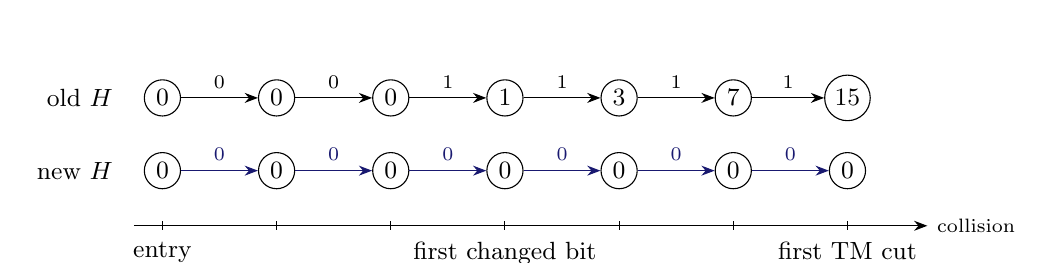
\begin{tikzpicture}[x=1.45cm,y=.56cm,>=Stealth,font=\small]
 \draw[->] (-.25,0)--(6.7,0) node[right]{\scriptsize collision};
 \foreach \x in {0,...,6} {\draw (\x,.1)--(\x,-.1);}
 \node[anchor=east] at(-.35,2.9){old $H$};
 \node[anchor=east] at(-.35,1.25){new $H$};
 \foreach \x/\v in {0/0,1/0,2/0,3/1,4/3,5/7,6/15}{
  \node[draw,circle,inner sep=2pt] (o\x) at(\x,2.9){\v};}
 \foreach \x in {0,...,6}{\node[draw,circle,inner sep=2pt] (n\x) at(\x,1.25){0};}
 \foreach \x/\y/\b in {0/1/0,1/2/0,2/3/1,3/4/1,4/5/1,5/6/1}{
  \draw[->] (o\x)--node[above,font=\scriptsize]{$\b$}(o\y);
  \draw[->,MidnightBlue] (n\x)--node[above,font=\scriptsize]{0}(n\y);}
 \node[below] at(0,-.15){entry};
 \node[below] at(3,-.15){first changed bit};
 \node[below] at(6,-.15){first TM cut};
\end{tikzpicture}
\caption{History at the six clean $T=0$ startup collisions, starting at
history zero. Edge labels are appended bits; each update is $H\mapsto2H+b$.
The numerical physical encoding amplifies the final old history to a factor
$7^{15}$. The drawing is a boundary diagram, not a physical trajectory.}
\label{fpa:st:fig:history}
\end{figure}

For $A=1$, \eqref{fpa:st:eq:startup} gives $138$. The old boundary history was
$15$, old five-counter startup took $142$ steps, and its exact predicted
literal clock was $79{,}936{,}151{,}060{,}302$. That old full physical run
was not traversed. Both the new formula and the old comparison are derived
from finite macro words and exact prime costs; only the new small literal
startup is also backed by direct full execution.

\subsection{No nonzero-scratch input is removed}
Let $T\geq0$ and $h_T=2^T-1$. The initial entry records zero. Each of the $T$
successful scratch decrements records one, preceded by its nonrecording
positive test. After $i$ clears the history is $2^i-1$. The zero exit and
four merge edges then append five zeros. Therefore
\begin{equation}
 H_{\rm new}=32(2^T-1),\qquad
 H_{\rm old}=32(2^T-1)+15,\qquad W=0.
 \label{fpa:st:eq:allT}
\end{equation}
The data at the end are $(L,R,0)$ in both machines.

The exact new five-counter clock is
\begin{align}
 P_5(T)
 &=4+\sum_{i=0}^{T-1}\bigl(10(2^i-1)+7\bigr)
       +\sum_{j=0}^{4}\bigl(10\cdot2^j h_T+4\bigr)\notag\\
 &=320\cdot2^T-296-3T.
 \label{fpa:st:eq:allTclock}
\end{align}
For $T=0$, the empty first sum gives $24$. The old five-counter clock is
exactly $P_5(T)+118$ for every natural $T$. One way to see the constant
$118$ is to compare the five final macros: their old added-history
increments are $0,1,3,7$ before the last four relevant costs, contributing
$10(0+1+3+7)$, plus four two-step preparations, for $110+8$.

At $T=1,L=R=0,C=1$, the new five-counter startup takes $341$ steps and ends
with $H=32$. Its composed literal clock is
\[
 18{,}595{,}602{,}803{,}420{,}561{,}611{,}627{,}873{,}065.
\]
This is a theorem-predicted value, not a traversed two-counter run.
Formula~\eqref{fpa:st:eq:startup} must not be applied to this input. Nonzero scratch
is fully supported semantically, but its recorded clearing history remains
in an exponent and can be prohibitive.

\section{The order preserving comparison proof}
\label{fpa:st:sec:dominance}
A smaller final history by itself does not prove a smaller runtime: the
intermediate work counter also enters the prime encoding. The needed
comparison matches actual primitive operations in chronological order.

\begin{lemma}[Recorded macro domination]
\label{fpa:st:lem:dominance}
Fix equal data and cofactor and an enabled normalized recording edge.
Let its old history be $h+d$ and new history $h$, with $h\geq0,d\geq1$,
and let the old and new tags be any $b_o,b_n\in\{0,1\}$. Its full old
literal two-counter duration is strictly larger than its new duration.
\end{lemma}
\begin{proof}
Match the common data operation, entry $Z_W$, and first $h$ transfer
iterations, preserving order. Each matched pair uses the same symbol and
counter, and the old encoded integer is $7^d$ times the new one. Then allow
the old run to perform its $d$ unmatched transfer iterations. Match the two
$Z_H$ exits; the ratio is now $11^d$.

Three bit cases are immediate. If both tags are one, match the two
preparation operations at ratio $11^d$. If both are zero, there are no
preparations. If $b_o=1,b_n=0$, leave the old preparation unmatched. In each
of these cases, let the old run complete $d$ surplus doubling iterations.
The two work counters now both equal $h$, and the old history exceeds the
new by $2d+b_o-b_n\geq1$. Match the remaining $h$ doubling iterations and
final $Z_W$; every encoding ratio is $7^{2d+b_o-b_n}\geq7$.

The case $b_o=0,b_n=1$ needs a different alignment. In the old run's first
doubling iteration, leave its $P_W,-W$ unmatched. Match the new preparation
$+H,P_H$ to the old iteration's \emph{first} $+H,P_H$ pair. Just before
these matches the old work exceeds the new by $d-1$, so the encoding ratio
is $11^{d-1}\geq1$. Finish that old iteration (its second $+H,P_H$ pair),
then complete the next $d-1$ old doubling iterations. Old and new work now
both equal $h$, while the old history is $2d$ and new history is $1$.
Match the new $h$ doubling iterations and exit to the old remainder at
ratio $7^{2d-1}\geq7$.

In every case, this is an order-preserving injection from new operations
into old operations. No old operation is used twice. Every matched pair has
the same prime and primitive, with old encoded integer at least new. The
exact costs \eqref{fpa:st:eq:primeclocks} are nondecreasing on those domains.
There are unmatched old positive-cost operations (in particular the extra
transfer iterations). Summing proves strict inequality.
\end{proof}

\begin{table}[htbp]
\centering\small
\begin{tabular}{@{}ccp{66mm}l@{}}
\toprule
$b_o$ & $b_n$ & Matching before the common doubling suffix & Final ratio\\
\midrule
0&0&Skip $d$ old doubling iterations &$7^{2d}$\\
1&1&Match preparation, then skip $d$ old iterations &$7^{2d}$\\
1&0&Skip old preparation and $d$ old iterations &$7^{2d+1}$\\
0&1&Match new preparation inside the first old iteration; finish $d$ old iterations in total &$7^{2d-1}$\\
\bottomrule
\end{tabular}
\caption{The four bit cases in the chronological matching. In the last row,
preparation is matched at ratio $11^{d-1}$ before the common suffix.}
\label{fpa:st:tab:embedding}
\end{table}

\begin{lemma}[The first strict gain]
\label{fpa:st:lem:first}
At equal incoming history, equal tags give equal costs. At equal history
with $b_o=1,b_n=0$, the old recorded macro is strictly longer.
\end{lemma}
\begin{proof}
Match the data operation, entry, transfer, and transfer exit. Skip the old
two preparation operations. The matched doubling suffix has the same work
but old history larger by one, so its encodings are larger by a factor of
seven. Monotonicity plus the skipped positive-cost operations proves the
strict claim, also when the doubling suffix is empty.
\end{proof}

\begin{proof}[Proof of the clock assertions in Theorem~\ref{fpa:st:thm:main}]
Both runs follow the same normalized data path. Throughout the common
scratch-clearing portion their histories and tags agree. The first changed
startup tag is old one/new zero, so Lemma~\ref{fpa:st:lem:first} yields the first
strict gain. Subsequent startup changes also have this favorable sign.
At the first TM cut, \eqref{fpa:st:eq:allT} gives a history difference $d=15$ for
every original loader input.

Afterward, a nonrecording edge leaves $d$ unchanged. On a recording edge,
\begin{equation}
 d'=2d+b_o-b_n\geq2d-1\geq d\geq15.
 \label{fpa:st:eq:gap}
\end{equation}
Thus the positive gap persists, whatever the later bit choices. Each
recorded macro is strictly improved by Lemma~\ref{fpa:st:lem:dominance}. For a
nonrecording edge, old and new use the same operation on equal data, and
old encoding is $7^d$ times new. Prime-cost monotonicity gives a nonlarger
new duration (an identity can tie). Induction on normalized edges proves
all cumulative inequalities. The strict gain already obtained in startup
persists to every TM cut.
\end{proof}

For an arithmetic cross-check, after the data operation put
$K=C2^L3^R5^T$. The exact costs of individual loop iterations are
\begin{align*}
\text{transfer at }(H,W)=(h-j,j):
 &\quad136K7^{h-j-1}11^j+12,\\
\text{doubling at }(H,W)=(b+2j,h-j):
 &\quad474K7^{b+2j}11^{h-j-1}+18,\\
\text{bit-one preparation after transfer}:
 &\quad46K11^h+6.
\end{align*}
Here a loop body is used only within its enabled iteration range. These
formulas are obtained by summing four, six, and two corresponding primitive
costs. They corroborate the embedding but do not replace its chronological
argument. The independent checker also tests 336 actual-row suffix embeddings,
covering all four bit pairs and several history gaps and cofactors.

\section{The exact optimum within the orientation class}
\label{fpa:st:sec:optimality}
There is a useful stronger conclusion, with a deliberately narrow comparison
class. Keep the normalized data program, recorder, prime encoding, and every
macro template fixed. An \emph{orientation} chooses one of the two bijections
to $\{0,1\}$ at each incoming recording pair. For this source there are
$2^{233}$ static orientations. This class changes labels only; it does not
vary algorithms, registers, primes, normalizations, or universal machines.

Fix a finite enabled normalized trace $e_1,\ldots,e_n$, including its data
values, and a common initial history $h_0\geq0$, $W=0$, and admissible
cofactor. Define a greedy orientation $G$: when an incoming edge first
traverses a previously unseen recording pair, assign that edge zero and its
companion one. Choices at pairs never traversed in the trace are arbitrary.
Merely starting at a pair's target does not count as encountering the pair.

\begin{theorem}[Finite-trace first-encounter optimality]
\label{fpa:st:thm:greedy}
Within the fixed orientation class, $G$ simultaneously minimizes the history
and the cumulative literal two-counter arrival clock at every normalized
boundary of the finite trace. If another orientation $O$ differs on any
encountered pair, then from its first such encounter onward its history and
cumulative clock are strictly larger. Orientations differing only on
unencountered pairs tie throughout the trace.
\end{theorem}
\begin{proof}
Two different orientations of a pair disagree on both incoming labels.
Thus their first disagreement along the trace must occur on the first
encounter of a pair. At that edge $G$ uses zero and $O$ uses one; incoming
histories agree, so the outgoing difference $H_O-H_G$ is one. A
nonrecording edge preserves this difference. A recording edge updates a
positive difference $d$ to
\[
 2d+b_O-b_G\geq2d-1\geq1.
\]
This includes later visits to either edge of the same pair. The history gap
therefore never closes.

Before the first disagreement, primitive operations and costs agree,
regardless of their private-control names. At that disagreement,
Lemma~\ref{fpa:st:lem:first} gives a strictly later alternative arrival. Afterward,
Lemma~\ref{fpa:st:lem:dominance} makes every alternative recorded macro strictly
longer, and prime-cost monotonicity makes every nonrecording edge no faster.
The cumulative strict gap persists. If there is no encountered disagreement,
all histories and clocks coincide. The termination ranks already proved
ensure that every finite arrival clock is defined.
\end{proof}

Equivalently, after $k$ recording events,
\[
 H_k=2^k h_0+\sum_{j=1}^{k}b_j2^{k-j}.
\]
The greedy feasible bit word is lexicographically smallest. Its leading
favorable difference outweighs all later forced opposite differences,
including repeated pair visits. This explains the history optimum; the
operation-embedding lemma is still essential for the literal-clock optimum.

\begin{corollary}[Every clean startup is optimal within this class]
\label{fpa:st:cor:optimalstartup}
For every original $L,R,T,C$ loader input, the present source minimizes
history and literal arrival time at every normalized startup prefix among
all $2^{233}$ orientations of the fixed templates. Exactly $2^{227}$ static
orientations attain the final startup minimum, counted as label assignments
rather than machines modulo isomorphism.
\end{corollary}
\begin{proof}
The normalized startup word for arbitrary natural $T$ is
\[
 \code{entry};\quad
 (\code{v0000p},\code{v0000d})^T;\quad
 \code{v0000z};\quad
 \code{n0001e0};\ \code{n0001e1};\ \code{n0001e2};\ \code{n0001e3}.
\]
The entry first encounters its pair, so it gets zero; later clearing
decrements use its companion and get one. The positive-test edges
\code{v0000p} are nonrecording. The next five distinct first encounters are
the zero exit and the four merge edges. Thus the same six zero choices in
Table~\ref{fpa:st:tab:swaps} are greedy for every $T$, independently of $L,R,C$.
Theorem~\ref{fpa:st:thm:greedy} applies. All six pairs are encountered even for
$T=0$, so a change on any of them is strictly worse by the final boundary.
The other 227 pairs are unused during startup and can be oriented freely.
\end{proof}

Consequently \eqref{fpa:st:eq:startup} is the exact minimum startup clock in this
class for every $T=0$ input; $138$ is its attained empty-input minimum.
This does not claim that the present orientations of the other 227 pairs
are optimal for later TM prefixes or simultaneously for all full inputs.
The theorem about this particular source and its predecessor remains
Theorem~\ref{fpa:st:thm:main}.

Given a finite trace, the greedy assignment is computed by one scan with a
set of encountered pairs. The resulting literal machine contains no
simulation callback or halting oracle. Nothing here supplies a uniformly
terminating procedure that compiles an optimal completed assignment for an
arbitrary infinite computation: an ongoing scan need not certify which
unseen pairs will never occur. No global machine/runtime optimality,
raw-CA optimum, or optimality beyond the fixed templates is asserted.
The separate proof and independent audit are bundled in
\code{reproducibility/orientation-addendum/}; they do not change any frozen
source or recorded execution bytes.

\section{The genuine equal history slowdown}
\label{fpa:st:sec:tradeoff}
The four companion edges in Table~\ref{fpa:st:tab:swaps} receive one instead of
zero. From \emph{equal} starting history $h$, each such macro now costs two
extra five-counter steps and ends at history $2h+1$ instead of $2h$. The
prime encoding can greatly magnify this local difference.

For example, execute the \code{v0303z} macro from
\code{tm\_I0\_0\_restore} with five-counter input $(0,0,0,0,0)$ and $C=1$.
The physical starting pair is $(1,0)$ in each machine. Direct literal replay
gives
\begin{center}
\begin{tabular}{@{}lrrl@{}}
\toprule
Machine & Literal steps & Final history & Final physical pair\\
\midrule
Frozen predecessor & 28 & 0 & $(1,0)$\\
New source & 104 & 1 & $(7,0)$\\
\bottomrule
\end{tabular}
\end{center}
Both reach \code{tm\_A0\_pop0}; both paths were traversed. This rules out
universal pointwise speedup from arbitrary internal states with equal
histories. It does not contradict Theorem~\ref{fpa:st:thm:main}: corresponding
clean-loader runs arrive here with old history already at least 15 larger.

More generally, along any fixed normalized path with $k$ recording events,
its history difference from an equal initial history is
\begin{equation}
 H_{\rm new}-H_{\rm old}
 =\sum_{j=1}^{k}(b_{n,j}-b_{o,j})2^{k-j}.
 \label{fpa:st:eq:arbitraryword}
\end{equation}
This expression may have either sign. The clean-loader theorem uses the
specific favorable startup and its persistent positive old-minus-new gap;
it does not infer a time comparison for arbitrary words from their final
history values alone.

\section{The executed 348 step prefix}
\label{fpa:st:sec:trace}
The literal interpreter evaluates the actual saved branch guards, selects
the unique enabled branch, changes one physical counter by its serialized
delta, and advances one control per step. It never jumps over a macro.
It traversed empty startup and one complete following TM transition in one
continuous run. All 348 source rows are recorded in the bundled
\code{empty-through-first-tm-literal-trace.json}.

\begin{figure}[htbp]
\centering
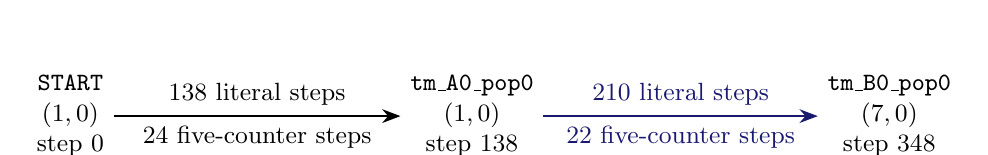
\begin{tikzpicture}[>=Stealth,font=\small]
 \node[align=center] (s) at(0,0){\code{START}\\$(1,0)$\\step $0$};
 \node[align=center] (a) at(5.1,0){\code{tm\_A0\_pop0}\\$(1,0)$\\step $138$};
 \node[align=center] (b) at(10.4,0){\code{tm\_B0\_pop0}\\$(7,0)$\\step $348$};
 \draw[->,thick] (s)--node[above]{138 literal steps}node[below]{24 five-counter steps}(a);
 \draw[->,thick,MidnightBlue] (a)--node[above]{210 literal steps}node[below]{22 five-counter steps}(b);
\end{tikzpicture}
\caption{The actual continuous source execution. Labels below the arrows
refer to a different simulation layer, not alternative counts of physical
steps. Exactly one TM transition occurs after the first cut.}
\end{figure}

\begin{table}[htbp]
\centering\small
\begin{tabular}{@{}lrrrl@{}}
\toprule
Arrival boundary & Five steps & Literal increment & Literal total & $(A,B)$\\
\midrule
\code{init\_clear\_T} & 4 & 22 & 22 & $(1,0)$\\
\code{n0001\_0} & 8 & 28 & 50 & $(1,0)$\\
\code{n0001\_1} & 12 & 22 & 72 & $(1,0)$\\
\code{n0001\_2} & 16 & 22 & 94 & $(1,0)$\\
\code{n0001\_3} & 20 & 22 & 116 & $(1,0)$\\
\code{tm\_A0\_pop0} & 24 & 22 & 138 & $(1,0)$\\
\code{tm\_B0\_pop0} & 46 & 210 & 348 & $(7,0)$\\
\bottomrule
\end{tabular}
\caption{A compact index into the saved trace. ``Five steps'' is cumulative
at the five-counter layer. ``Literal increment'' is the duration since the
preceding listed boundary. No individual physical row is omitted from the
machine-readable trace.}
\end{table}

At the empty input, each identity costs one literal step and every zero test
in the startup costs seven. The first history macro has one identity and
three tests, costing $22$; the second has four tests, costing $28$; each of
the last four again costs $22$. Their sum is $138$.

The first TM transition has four independent three-counter instructions and
22 five-counter steps. Its first four history macros have zero tags and
cost $28$ literal steps each. The last has bit one and its six primitive
costs are $1,7,7,17,35,31$, totaling $98$. Thus the literal duration is
$4\cdot28+98=210$. It reaches state $B$ scanning zero, with
$(L,R,T,H,W)=(0,0,0,1,0)$, hence physical $(7,0)$. This is a finite prefix,
not a completed universal program or evidence of efficient general simulation.

\begin{table}[htbp]
\centering
\begin{tabular}{@{}lrrr@{}}
\toprule
Executed segment & Zero updates & Decrements & Increments\\
\midrule
Startup & 100 & 19 & 19\\
First TM transition & 134 & 35 & 41\\
Continuous prefix & 234 & 54 & 60\\
\bottomrule
\end{tabular}
\caption{Serialized branch census. The rows sum to 138, 210, and 348,
respectively. ``Zero update'' includes tests and identities.}
\end{table}

The producer also traversed five other clean startups, at $A=2,3,13,72,78$,
with respective literal clocks $214,290,1130,6118,6650$. The independent
checker traversed 13 clean startups at
$A=1,2,3,4,6,9,13,17,26,27,81,243,351$; for $A=351$ the exact count is
$29{,}706$. These finite cases corroborate Proposition~\ref{fpa:st:prop:startup};
the 24-operation decomposition proves it for every allowed $A$.

\section{The binary compiler and the limits of the clock claim}
\label{fpa:st:sec:ca}
The unchanged strict compiler uses the numerical parameters
\[
 m=122622,\quad p=66066,\quad a=75495,\quad J=0,
\]
\[
 D=509508,\qquad S=1019018,\qquad Z=20380380.
\]
Its indexed construction still has $269{,}291{,}358{,}255$ local involution
factors and radius upper bound $3{,}292{,}955{,}588{,}459{,}274{,}804$.
The binary alphabet and five-particle encoding are unchanged. Empty input
is loaded at positions
\[
 \{-20380381,\ 0,\ 1019018,\ 1019019,\ 20380380\}.
\]
The source table differs, so this is a new indexed CA rule despite identical
geometry. No equality or conjugacy of its global map with the predecessor's
map is asserted.

For the unchanged compiler, a source zero update takes one CA microedge. A
source move with pre-move selected physical counter $c$ and
$\delta\in\{-1,1\}$ takes
\begin{equation}
 3+2(Z+c)+\delta-4S
 \label{fpa:st:eq:caclock}
\end{equation}
microedges. Summing this theorem-derived expression over the actually
executed source trace gives:
\begin{center}
\begin{tabular}{@{}lr@{}}
\toprule
Source segment & Predicted CA microedges\\
\midrule
Empty startup & 1,394,018,396\\
First TM transition only & 2,788,036,936\\
Through first TM transition & 4,182,055,332\\
\bottomrule
\end{tabular}
\end{center}
These are exact predicted CA clocks. No CA microedge run was traversed and
no full factor array was allocated. In particular, a count of fewer literal
steps does not by itself compare sums of \eqref{fpa:st:eq:caclock}, whose costs
also depend on intermediate physical counters. This report proves no old/new
raw-CA speed comparison and gives no uniform speedup ratio.

The source properties needed for the earlier binary composition are retained:
partial injection, predecessor-free start, terminal halt, and nonblocking
infinite continuation on clean inputs. Thus the existing periodicity argument
applies separately to the new CA instance. If a finite source run has total
CA microedge clock $\Theta$, its signed orbit has least period $2\Theta+2$;
if the source continues forever, the initial encoded configuration never
returns. The no-incoming start and partial injection exclude a repeated
unsigned forward node. This is proof inheritance through a newly verified
source, not an execution of a universal CA instance. The separate four-mass
lower-bound theorem of Report 12 is not re-proved or needed for the startup
comparison here.

\section{Reproducibility and provenance}
\label{fpa:st:sec:replay}
The portable bundle has three roles: this editable \LaTeX\ report and its
PDF; the exact source, proofs, traces, and reconstruction checks in
\code{reproducibility/}; and release-wide byte manifests. All runtime
references are relative to the extracted bundle. Verification requires
Python 3 and its standard library, and no network. Rebuilding this PDF
additionally requires a \LaTeX\ installation with the packages named in
its preamble.

The pinned source dependency is the 528-instruction three-counter program
for the Neary--Woods 15-state, two-symbol universal TM \cite{fpa:nw}.
Its source rows, normalization, and input encoding are unchanged. The
published finite-input universality theorem is an inherited mathematical
dependency. The bundled transition table and entry-by-entry comparison do
not purport to re-prove that published theorem. The earlier primary visual
check covered printed pages 112 and 121, including all 30 transition cells
and the initial scanned blank. The undefined transition is state $J$
scanning one. No new third-party PDF is bundled.

The history and prime constructions follow Morita's reversible-counter
method \cite{fpa:morita1996}, but their exact local graphs are independently
reconstructed and proved here. The prior primary scan was not visually
verified: the available endpoint returned HTML and screenshots failed.
No claim relies on resolving an ambiguous OCR symbol. These inherited
provenance limits remain explicit.

The checks have distinct logical jobs:
\begin{enumerate}
\item Reconstruct the primitive and normalized three-counter graph from
pinned input; verify the complete source simulation and its affine paths.
\item Verify every per-pair label bijection, reconstruct the full
five-counter graph, and reconstruct every expanded two-counter prime graph.
\item Check complete edge multisets, private-state separation, signed
serialization, global domain/image separation, and START/HALT conditions.
\item Independently derive the exact four relabelings from actual normalized
rows and compare against mandatory pinned predecessor inputs.
\item Traverse the startup and 348-step source prefix; check the nonzero-$T$
five-counter formulas, equal-history counterexample, and 336 suffix embeddings.
\item Rebuild all seven generated source outputs byte-for-byte, then replay
all checks both normally and with Python's optimization flag enabled.
\end{enumerate}
The checker uses explicit failure conditions rather than relying on
assertions that disappear under \code{-O}. The broader macro audit includes
2,330 history and 27,743 prime sample runs; the targeted relabel audit adds
1,398 history traces and eight five-counter prologues for $T=0,\ldots,7$.
Finite sample counts are supplemental evidence. The unbounded proofs are
the checked complete graphs together with their invariants and ranks.

Consult \code{reproducibility/README.md} for the exact replay commands and
\code{PORTABILITY.md} there for the adaptation ledger. Baseline files are
bundled and SHA-pinned; a missing baseline is a failure, not a reason to skip
the comparison. Any retained historical receipt is explicitly bounded to
its original role and labeled if adapted. Fresh portable replay receipts
attest to the shipped checkers, not to an undocumented external workspace.

The orientation addendum is a separate independently checked mathematical
argument. Its two notes and seal are verified as file dependencies; this hash
check does not mechanically prove their theorems or add literal-execution
coverage.

\begin{samepage}
The complete trace SHA-256 is
\begin{center}\small\ttfamily
6f6374db5fb0f8ce1de3afb628cbee1e46c354ad98d88b0d2c278601f6005e4d
\end{center}
\end{samepage}
\begin{samepage}
The new reversible-five graph SHA-256 is
\begin{center}\small\ttfamily
2f426dda9743a80d1677bf367f4c75b1522efbd31cd6f07ab59ff7643b4ed31f
\end{center}
\end{samepage}
The outer manifest covers the actual shipped files and excludes only itself
and its detached checksum to avoid self-reference. The archive has its own
separately recorded SHA-256. No developer logs, caches, absolute workstation
paths, or optional cross-release reads are part of the portable package.

\section{What is resolved and what remains useful}\label{fpa:rep:17:last}
\label{fpa:st:sec:questions}
\textbf{Does choosing zero lose reversibility?} No. The colliding pair still
has distinct zero/one labels, and every global join is rechecked. A repeated
zero history value at different controls is not a collision of complete
configurations.

\textbf{Does this quietly narrow the loader?} No. Equations
\eqref{fpa:st:eq:allT}--\eqref{fpa:st:eq:allTclock} cover all initial natural scratch, and
all original $L,R,C$ choices survive. The small formula
\eqref{fpa:st:eq:startup} is expressly restricted to $T=0$.

\textbf{Is the improvement only a startup benchmark?} No. The history-gap
recurrence and chronological embedding prove a whole-prefix comparison at
corresponding boundaries from every clean loader input. However, later
history can still become enormous, so the theorem supplies no practical
runtime guarantee for arbitrary universal programs.

\textbf{Can every internal state be made faster?} This particular change
cannot: the fully executed companion example costs 104 instead of 28 steps
at equal history. For a specified finite workload trace, Theorem~\ref{fpa:st:thm:greedy} gives the
optimal orientation within these fixed templates. That conclusion does not
optimize arbitrary internal inputs or changes to the recorder itself.

\textbf{What would make the next computation useful?} A sensible next target
is another explicitly bounded literal TM prefix with complete trace
accounting. One should first compute its five-counter and prime-expanded
clock to determine whether literal replay is feasible. This report stops at
the one transition that was actually executed; no pending run is presented
as a result.

\textbf{What remains at the CA layer?} A lazy indexed compiler or evaluator
would avoid eagerly allocating hundreds of billions of factors, but would
need its own semantic and indexing audit. A genuine old/new CA clock
comparison needs a separate argument controlling intermediate physical
counter values and move counts, not just Theorem~\ref{fpa:st:thm:main}. Those are
concrete next questions, not claimed consequences of the present proof.

\wtag\ Both questions are answered in this report: Report~18 (second half of this Part) gives the old/new comparison in the automaton's clock (Theorem~\ref{fpa:cc:thm:oldnew}), and Report~19 (Part~\ref{fpa:part:four}) the lazy evaluator (Theorem~\ref{fpa:lz:thm:main}).

\textbf{Bottom line.} A local, admissible choice of four history labels
preserves the complete original semantics and geometry while removing a
specific catastrophic clean-startup cost. The executed result is a 348-step
literal prefix. The stronger unbounded result is paired clean-input
boundary domination. Their evidence and limitations are deliberately kept
distinct.

\reportopening{18}{Cellular clocks for a literal reversible source}{Exact macro costs and first encounter domination}{Report 18 \quad Separate proof and reproducible audit}

\begin{reportabstract}{18}
The four history-tag swaps in Report 17 improve not only literal two-counter
arrival times but also the cellular-automaton clock of its fixed strict binary
compiler. The key identity is
$\Theta=\lam M+\TV(A^2)+\TV(B^2)+U$, with
$\lam=36{,}684{,}691$, moving-row count $M$, and zero-update count $U$.
Exact whole-prime macro costs are increasing in their enabled encoded input.
A proof that all $2^{233}$ static history orientations have the same compiler
constant then lifts the recorder's operation embedding to a CA-clock
comparison. For a fixed finite normalized trace, assigning zero to each
pair's first encountered edge minimizes every boundary arrival time at once.
Exactly $2^{227}$ assignments attain the complete clean-startup minimum
for every promised loader input. For zero initial scratch, that minimum
has an explicit quadratic and floor formula. The empty startup takes
138 executed literal rows and exactly 1,394,018,396 theorem-derived CA
microedges. The continuous executed source prefix has 348 rows and covers
one TM transition; no CA orbit or giant rule array was executed.
An independent graph reconstruction and normal and optimized Python replays
support the proof. The portable bundle preserves the exact scientific
source bytes and includes a mandatory pinned predecessor reconstruction.
\end{reportabstract}

\textbf{What changes.} This report settles the CA-clock comparison left open
by Report 17 within its fixed static-orientation, recorder, prime-template,
and compiler class. It does not change the Report 17 source. The two
compared CA rules can differ despite equal numerical geometry.

\textbf{Evidence and scope.} These are mathematical proofs with independent
executable audits, not proof-assistant formalizations. No novelty, optimal
universal-machine size, unrestricted speedup, or host-runtime claim is made.
A clock unit is one iteration of the compiled CA on its admissible forward
plus orbit, not one evaluation of an individual factor of its local rule.

\wtag\ Delivered as \path{Cellular_Clock_Domination_Package.zip} (batch~82, archive~04; arrival \texttt{db37d18c8}), dated 3~October 2026; files placed by \texttt{bca6383e9} with the prefix given in Appendix~\ref{fpa:app:provenance}. Report~18 continues Report~17 (first half of this Part) and settles the cellular-clock comparison that Report~17 left open.

\section{The comparison and its domain}\label{fpa:rep:18:first}
\label{fpa:cc:sec:main}
The normalized three-counter program has data $(L,R,T)\in\N^3$. Its fixed
recorder adds history $H$ and work $W$. A five-counter boundary is represented
in the literal two-counter machine by
\begin{equation}
 (A,B)=\bigl(C2^L3^R5^T7^H11^W,0\bigr),\quad
 C\geq1,\quad \gcd(C,2310)=1.
 \label{fpa:cc:eq:encoding}
\end{equation}
The clean-loader domain is $H=W=0$; it includes every natural initial
scratch value $T$, not just $T=0$. Every literal row is an increment,
enabled decrement, zero test, positive test, or identity. Tests cost time.

Let $\mathcal O$ consist of the $2^{233}$ static orientations of the 233
incoming collision pairs. An orientation gives distinct bits zero and one
to the two members of each pair. The normalized program, recorder,
prime order $(2,3,5,7,11)$, literal macro templates, and strict binary-five
compiler are fixed. Every member retains the recorder's global partial
injection and its enabled-macro completion property. Arrival times below
are at completed normalized-source edges, not at arbitrary internal rows.

\begin{theorem}[First encounter prefix optimality]
\label{fpa:cc:thm:optimal}
Fix a finite enabled normalized trace, common initial data, common history
$h_0\in\N$, clean work $W=0$, and common cofactor $C$ as in
\eqref{fpa:cc:eq:encoding}. Choose $G\in\mathcal O$ to give bit zero to the first
encountered edge of each used pair. Then $G$ minimizes cumulative CA arrival
time at every normalized boundary simultaneously. A competitor ties through
a prefix exactly when it agrees with $G$ on all pairs encountered in that
prefix. At its first encountered disagreement it becomes strictly slower,
and it remains strictly slower at every subsequent boundary.
\end{theorem}

\wtag\ The literal-clock statement is Theorem~\ref{fpa:st:thm:greedy} of Report~17.

\begin{theorem}[The frozen optimized and predecessor sources]
\label{fpa:cc:thm:oldnew}
On every common input $(\START,C2^L3^R5^T,0)$ in the clean-loader domain,
the Report 17 source reaches every corresponding normalized boundary no
later in CA microedges than the Report 16 predecessor. It arrives strictly
earlier by the first TM cut, and at every later corresponding boundary.
The assertion holds for every finite prefix, whether or not the run halts.
\end{theorem}

\wtag\ The literal-clock statement is Theorem~\ref{fpa:st:thm:main} of Report~17; this theorem answers the comparison that Report~17 left open (Section~\ref{fpa:st:sec:questions}).

A TM cut requires the designated TM control and $T=0$. A loop visit to a
cut label with nonzero scratch is not such a cut. Both sources have the
same normalized data trace, including the same TM transitions.

These theorems compare different fixed rules at matching semantic
boundaries. They do not order arbitrary equal-history internal states or
all intermediate physical configurations. They assert no equal-time
alignment, conjugacy, fixed speedup ratio, or globally optimal construction.
The finite trace in Theorem~\ref{fpa:cc:thm:optimal} is supplied; no halting decision
procedure or uniform discovery of an arbitrary infinite run's first
encounters follows.
\newpage

\section{An exact total variation identity}
\label{fpa:cc:sec:variation}
The inherited strict compiler subdivides a moving literal row, with old
selected counter $c$ and update $\delta\in\{-1,+1\}$, into dispatch,
outward travel, endpoint move, return travel, and commit. Their durations are
\[
 1,\quad Z+c-2S,\quad 1,\quad Z+c+\delta-2S,\quad 1.
\]
Thus its exact microedge clock is
\begin{equation}
 \tau(c,\delta)=3+2(Z+c)+\delta-4S
 =\lam+\left|(c+\delta)^2-c^2\right|,
 \qquad \lam=3+2Z-4S.
 \label{fpa:cc:eq:rowtime}
\end{equation}
For an increment $c\geq0$, the absolute difference is $2c+1$. For an enabled
decrement $c\geq1$, it is $2c-1$. A disabled decrement is not covered.
Every zero-update row, including each successful test and identity, takes
exactly one microedge.

\wtag\ Equation~\eqref{fpa:cc:eq:rowtime} is Report~15's clock~(5) (Section~\ref{fpa:sec:micrograph}) and Report~16's \eqref{fpa:ls:eq:caclock}, written as a total variation.

\begin{proposition}[Exact path clock]
\label{fpa:cc:prop:tv}
For every finite enabled literal path, let $M$ count moving rows and $U$
count zero-update rows. If $(A_t,B_t)$ are its actual physical counters, then
\begin{equation}
 \Theta=\lam M+\sum_t|A_{t+1}^2-A_t^2|
                   +\sum_t|B_{t+1}^2-B_t^2|+U
       =\lam M+\TV(A^2)+\TV(B^2)+U.
 \label{fpa:cc:eq:tv}
\end{equation}
\end{proposition}
\begin{proof}
Sum \eqref{fpa:cc:eq:rowtime} over moving rows and add one for each zero update.
Only the selected physical counter changes in a moving row, while neither
changes in a test or identity. Every row is counted once.
\end{proof}

Total variation must not be replaced by the endpoint difference of squares.
For example, a counter moving $N\to0\to N$ contributes $2N^2$, although
its endpoints agree. This distinction is why literal instruction-count
improvement alone was insufficient to establish CA-clock improvement.

\begin{figure}[htbp]
\centering
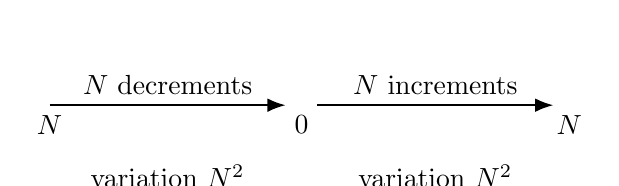
\begin{tikzpicture}[>=Latex,thick,x=1cm,y=1cm]
\draw[->] (0,0)--(3,0) node[midway,above] {$N$ decrements};
\draw[->] (3.4,0)--(6.4,0) node[midway,above] {$N$ increments};
\node[below] at (0,0) {$N$};\node[below] at (3.2,0) {$0$};\node[below] at (6.6,0) {$N$};
\node at (1.5,-.9) {variation $N^2$};\node at (4.9,-.9) {variation $N^2$};
\end{tikzpicture}
\caption{A return to the same counter value still contributes positive clock.}
\end{figure}

Writing $m$ for controls and $p_{\rm move}$ for moving rows, the compiler has
\[
 D=2(m+2p_{\rm move}),\qquad S=2D+2,\qquad Z=40D+60+2J,
 \qquad \lam=72D+115+4J>0.
\]
For the present class, $m=122622$, $p_{\rm move}=66066$, $J=0$,
$D=509508$, $S=1019018$, and $Z=20380380$, so
$\lam=36{,}684{,}691$. Section~\ref{fpa:cc:sec:invariance} proves that these values
are common to every compared orientation.
\newpage

\section{Whole prime macros from their literal paths}
\label{fpa:cc:sec:macros}
A five-counter operation at prime $p\in\{2,3,5,7,11\}$ begins with physical
counters $(N,0)$, $N>0$. Other encoded exponents are arbitrary naturals.
An enabled decrement or positive test requires $p\mid N$; an enabled zero
test requires $p\nmid N$. We count the entire macro through its restored
five-counter boundary, including its destination restorer.

\subsection{Increment and enabled decrement}
For increment, the first phase transfers $N$ units from $A$ to $B$; the
second removes each $B$ unit and increments $A$ exactly $p$ times. Hence
$A:N\to0\to pN$ and $B:0\to N\to0$. The exact counts are
\[
 M=(p+3)N,\qquad \TV(A^2)+\TV(B^2)=(p^2+3)N^2,\qquad U=4N+3.
\]
The three isolated tests are entry $B=0$, transfer exit $A=0$, and final
$B=0$. The transfer and return iterations each contribute two positive
tests. Therefore
\begin{equation}
 I_p(N)=(p^2+3)N^2+\lam(p+3)N+4N+3.
 \label{fpa:cc:eq:inc}
\end{equation}

For enabled decrement put $N=pQ$. The return loop removes $p$ units of $B$
per iteration and adds one to $A$, so $A:N\to0\to Q$ and $B:0\to N\to0$.
Every individual decrement in a $p$-block is charged. Divisibility prevents
an incomplete block. We obtain
\[
 M=3N+Q,\qquad \TV(A^2)+\TV(B^2)=3N^2+Q^2,\qquad U=2N+2Q+3,
\]
\begin{equation}
 D_p(N)=3N^2+Q^2+\lam(3N+Q)+2N+2Q+3.
 \label{fpa:cc:eq:dec}
\end{equation}

\subsection{Successful zero and positive tests}
Write $N=pQ+r$, $0\leq r<p$. The scanner decrements $A$ unit by unit,
tracks residue in finite control, and increments $B$ once per full block.
It exits at $(0,Q)$. Restoration first adds back $r$, then adds $p$ units
for each removed unit of $B$, ending at $(N,0)$. Consequently
\[
 M=2(N+Q),\quad \TV(A^2)+\TV(B^2)=2(N^2+Q^2),\quad U=2(N+Q)+3,
\]
\begin{equation}
 T_p(N)=2(N^2+Q^2)+2(\lam+1)(N+Q)+3,
 \qquad Q=\floor{N/p}.
 \label{fpa:cc:eq:test}
\end{equation}
The zero updates are one entry test, $N+Q$ scanner positive tests, one
scanner exit, $N+Q$ restoration positive tests, and one final test. The
formula includes restoration exactly once and is valid when $Q=0$.
It applies only to the selected successful branch. A wrong singleton test
blocks; we assign it no successful-boundary clock. An identity costs one.

These formulas evaluate exact paths in the serialized source. No repeated
arithmetic, division, residue test, or restoration becomes a unit-cost
operation of the simulated machine.
\newpage

\section{Monotonicity and the common compiler constant}
\label{fpa:cc:sec:invariance}
\begin{lemma}[Whole macro monotonicity]
\label{fpa:cc:lem:monotone}
For every real $\lam>0$, a fixed prime and a fixed successful primitive,
the whole macro clock is nondecreasing in its positive encoded input,
restricted to that primitive's enabled domain. It is strictly increasing
for increments, decrements, and tests; identity is constant. All costs are
positive.
\end{lemma}
\begin{proof}
All nonconstant coefficients of \eqref{fpa:cc:eq:inc} are positive. Substituting
$N=pQ$ in \eqref{fpa:cc:eq:dec} gives
$(3p^2+1)Q^2+[\lam(3p+1)+2p+2]Q+3$, strictly increasing for positive $Q$.
In \eqref{fpa:cc:eq:test}, both $N$ and $\floor{N/p}$ are nondecreasing and the
$N^2$ contribution strictly increases. Restriction to either enabled test
domain preserves the inequality. Identity has clock one.
\end{proof}

Comparing formulas with a common $\lam$ requires more than the observation
that the five-counter row count is unchanged. In particular, the literal
compiler shares restore blocks by destination. We prove the stronger
invariant needed to count those blocks.

At a collision pair, flipping orientation exchanges the two original
source-operation payloads feeding private bit-zero and bit-one entry
controls. The two transfer graphs and their shared doubling graph remain
fixed. Each original operation still appears once at its original source
and has the same selected counter and symbol. Therefore the multiset of
outgoing source groups, classified by prime and operation kind, is unchanged.

Every swapped source row has its own private entry destination. Exchanging
the two rows merely permutes whether each entry needs restoration, and for
which prime. It preserves the multiset of restorer primes. Other recorder
destinations and nonrecording destinations are fixed. The argument holds
after any set of other flips, so it covers all $2^{233}$ orientations.

\begin{center}\small
\begin{tabular}{@{}lrrr@{}}
\toprule
Template at prime $p$ & New controls & Literal rows & Moving rows\\
\midrule
Identity & 0 & 1 & 0\\
Increment or decrement & $p+7$ & $p+10$ & $p+3$\\
Test group $E$ & $2p+2$ & $2p+3+(p-1)\mathbf1_{Z\in E}+\mathbf1_{P\in E}$ & $p+1$\\
Destination restorer & $2p+2$ & $2p+3$ & $p+1$\\
\bottomrule
\end{tabular}
\end{center}

Distinct prefixes keep private controls disjoint. Include the 4,520
five-counter controls once. Summing these invariant signatures gives
122,622 literal controls and 141,561 rows: 33,436 increments, 32,630
decrements, 23,429 zero tests, 52,036 positive tests, and 30 identities.
There are 2,330 shared restorers, with counts $(116,116,234,932,932)$ at
primes $(2,3,5,7,11)$. The guard grammar always has class cut $J=0$.
Thus $m,p_{\rm move},a,J$, where $a=75{,}495$ counts zero-update rows,
and hence $D,S,Z,\lam$, are identical.

The indexed rules and row order may differ. The common symbolic factor
count and radius bound do not identify the rules or constitute an executed
CA construction. All-orientation invariance follows from the local proof;
233 individual flips and the all-flipped check corroborate it.
\newpage

\section{The recorder embedding charges complete CA macros}
\label{fpa:cc:sec:embedding}
A recording edge with incoming history $h$ and assigned bit $b$ has word
\begin{align*}
 &\text{source operation};\quad W=0;\\[-3pt]
 &(H>0,H-,W+,W>0)^h;\quad H=0;\\[-3pt]
 &(H+,H>0)^b;\quad
 (W>0,W-,H+,H>0,H+,H>0)^h;\quad W=0.
\end{align*}
Here every displayed test is a separate five-counter primitive. The recorder
ends at $(H,W)=(2h+b,0)$. Compare a higher run with history $h+d$ and bit
$a$ to a lower run with history $h$ and bit $b$, with equal data and $d\geq1$.

\begin{lemma}[Strict recording clock domination]
\label{fpa:cc:lem:record}
For all four bit pairs $(a,b)$, the higher-history recording edge has a
strictly larger whole CA clock. At equal history, bit one costs strictly
more than bit zero, and equal bits have equal clocks.
\end{lemma}
\begin{proof}
Construct an order-preserving injection of lower operations into higher
operations, matching the same symbol and selected prime:
\begin{enumerate}
\item Match the source operation, entry test $W=0$, and the first $h$
transfer iterations. The higher encoded input is $7^d$ times the lower.
\item Skip the higher run's $d$ surplus transfer iterations and match
$H=0$. The encoded ratio is now $11^d$.
\item If $a=b=1$, match preparation at ratio $11^d$. If $(a,b)=(1,0)$,
skip the higher preparation. If $(a,b)=(0,0)$, neither has preparation.
In these cases skip $d$ higher doubling iterations.
\item In the remaining case $(a,b)=(0,1)$, skip $W>0,W-$ in the first
higher doubling iteration. Match the lower preparation $H+,H>0$ to that
iteration's first such pair, at ratio $11^{d-1}\geq1$. Finish that higher
iteration and the following $d-1$ surplus iterations.
\item Both runs now have work $W=h$. The history gap is $2d+a-b\geq1$.
Match their remaining $h$ doubling iterations and final test at encoded
ratio $7^{2d+a-b}\geq7$.
\end{enumerate}
Every lower operation is matched exactly once, both matched operations are
enabled, and the higher encoded input is no smaller. Lemma~\ref{fpa:cc:lem:monotone}
compares their complete literal expansions in CA time, using the common
$\lam$ proved above. Unmatched higher operations have positive costs;
in particular its surplus transfer iterations exist. This makes the total
inequality strict. At equal history and bits, the words coincide. At equal
history with bits one and zero, skip the bit-one preparation and match
the doubling suffix and final test at history gap one, again strictly.
\end{proof}

\wtag\ Lemma~\ref{fpa:st:lem:dominance} of Report~17 is the same embedding for the literal clock; the startup history used below is Report~17's equation~\eqref{fpa:st:eq:allT}, not re-derived.

For a nonrecording edge the same data operation at larger history has
nondecreasing cost; identity may tie. The proof aligns whole five-counter
primitives. It does not require pointwise alignment of the intermediate
physical counters inside their literal prime expansions.
\newpage

\section{Prefix optimality and the four startup swaps}
\label{fpa:cc:sec:prefix}
\begin{proof}[Proof of Theorem~\ref{fpa:cc:thm:optimal}]
Before the first encountered differing pair, the two histories, operations,
and clocks coincide. The first differing edge must be that pair's first
encounter: swapping orientation changes both of its edge labels. The
first-encounter orientation uses zero there, while its competitor uses one.
Lemma~\ref{fpa:cc:lem:record} creates history gap one and a strict clock delay.

At each later recording edge the competitor's history gap satisfies
\begin{equation}
 d'=2d+b_{\rm competitor}-b_G\geq2d-1\geq d\geq1.
 \label{fpa:cc:eq:gap}
\end{equation}
The higher-history macro costs strictly more, for either pair of current
bits. A nonrecording edge preserves the history gap and has no smaller
clock. Therefore the cumulative delay cannot shrink. This proves every
prefix inequality and the stated equality characterization, including
repeated visits. Every finite enabled macro completes, so all compared
finite arrival times are well-defined.
\end{proof}

If a finite trace encounters $k$ distinct collision pairs, precisely
$2^{233-k}$ orientations minimize its complete-trace clock; all of them
also minimize every prefix clock. Unencountered assignments cannot affect
the trace. This counts static assignments, not isomorphism classes of
machines.

For every clean prologue, the first-encounter members are the same six:
\code{entry}, \code{v0000z}, \code{n0001e0}, \code{n0001e1},
\code{n0001e2}, and \code{n0001e3}. The Report 17 orientation assigns zero
to all six. The first two already had zero in its predecessor; exactly four
pairs were swapped. The other 227 assignments are irrelevant to startup.
Consequently exactly $2^{227}$ orientations attain the complete startup
minimum for every clean-loader input simultaneously.

\begin{proof}[Proof of Theorem~\ref{fpa:cc:thm:oldnew}]
The two frozen sources follow the same normalized data/control trace.
Their histories agree until the first changed startup assignment, which
has old bit one and new bit zero. Its old clock is strictly greater.
The common clearing loop ends with history $2^T-1$. The following five
recording edges give
\begin{equation}
 H_{\rm old}=32(2^T-1)+15,\qquad
 H_{\rm new}=32(2^T-1).
 \label{fpa:cc:eq:startup-history}
\end{equation}
Thus by the first TM cut the old history exceeds the new by exactly 15.
Thereafter \eqref{fpa:cc:eq:gap}, now with the old and new bits, preserves a gap
of at least 15. Recording macros cost more in the old run and nonrecording
macros no less. Induction gives the claim for every later finite boundary.
\end{proof}

This second theorem does not assume that the Report 17 orientation is
first-encounter optimal on every later computation. Its all-later-boundary
comparison follows from the already established positive history gap.
The scope remains paired clean inputs; unrelated equal-history internal
states are not a substitute for that hypothesis.
\newpage

\section{The exact minimum when initial scratch is zero}
\label{fpa:cc:sec:startup}
For $T=0$ write $A=C2^L3^R$ and $q_p=\floor{A/p}$. The optimized five-counter
startup has five identities and nineteen successful zero tests: one at
prime 5, six at prime 7, and twelve at prime 11. All occur at the same
encoded integer $A$ because all six first-encounter bits are zero. The
loader's coprimality and $T=H=W=0$ make these tests enabled.

\begin{proposition}[Closed clean startup clock]
The exact minimum CA startup time in $\mathcal O$ for $T=0$ is
\begin{align}
 \Theta_0(A)={}&38A^2+2q_5^2+12q_7^2+24q_{11}^2\notag\\
 &+2(\lam+1)(19A+q_5+6q_7+12q_{11})+62.
 \label{fpa:cc:eq:startupclock}
\end{align}
\end{proposition}
\begin{proof}
The startup costs $5+T_5(A)+6T_7(A)+12T_{11}(A)$. Substitute
\eqref{fpa:cc:eq:test} and collect terms. The constant is $5+3(1+6+12)=62$.
First-encounter optimality makes this achieved value the class minimum.
\end{proof}

At empty input, $A=1$, all three quotients vanish, so
\begin{equation}
 \Theta_0(1)=38\lam+138=1{,}394{,}018{,}396.
 \label{fpa:cc:eq:empty}
\end{equation}
The source actually takes 138 literal rows: 38 moves and 100 zero updates.
Their total square variation is 38, agreeing with
$\lam\cdot38+38+100$. The large CA count is derived from the compiler
travel-time theorem. The CA itself was not iterated that many times.

\begin{center}
\begin{tabular}{@{}lrr@{}}
\toprule
Executed source segment & Literal rows & Derived CA microedges\\
\midrule
Empty startup & 138 & 1,394,018,396\\
Next TM transition & 210 & 2,788,036,936\\
Continuous prefix & 348 & 4,182,055,332\\
\bottomrule
\end{tabular}
\end{center}

The third row is the continuous union of the first two segments, not a
third disjoint execution. The first transition ends at control
\code{tm\_B0\_pop0} with physical counters $(7,0)$, representing one unit
of history and zero data. The earlier cut is \code{tm\_A0\_pop0} at $(1,0)$.
Only one TM transition beyond startup is certified by this saved trace.

Formula~\eqref{fpa:cc:eq:startupclock} must not be used for $T>0$. Although the
same six choices minimize all promised startups, positive scratch drives
history growth according to \eqref{fpa:cc:eq:startup-history}. Optimality within
a fixed class does not make those clocks small.

\textbf{Input cost boundary.} Arithmetic performed by the simulated
machine is fully charged. Constructing the initial integer $C2^L3^R5^T$
and writing its spatial encoding are external input preparation. The host
arithmetic used to evaluate a formula is not claimed to be CA computation.
\newpage

\section{An exact formula for the recorded suffix}
\label{fpa:cc:sec:suffix}
The following formula is useful for exact arithmetic without enumerating
an enormous literal or CA path. It excludes the original normalized data
operation. Let $K=C2^L3^R5^T$ be the data factor \emph{after} that operation;
then $\gcd(K,77)=1$. The suffix starts at $(H,W)=(h,0)$ and uses bit $b$.
Here $K$ is a data factor, not an instruction horizon.

For one transfer iteration, let $X$ be the encoded integer immediately
after its $H-$ operation. For one doubling iteration let $Y$ be the
encoded integer immediately after $W-$. If $V$ is the input to bit-one
preparation, the whole phase costs are
\begin{align}
 \mathcal T(X)&=616X^2+(76\lam+60)X+12,\label{fpa:cc:eq:transfer}\\
 \mathcal D(Y)&=8208Y^2+(266\lam+208)Y+18,\label{fpa:cc:eq:double}\\
 \mathcal P(V)&=152V^2+(26\lam+20)V+6.\label{fpa:cc:eq:prepare}
\end{align}
Each is obtained by summing \eqref{fpa:cc:eq:inc}--\eqref{fpa:cc:eq:test} for every
primitive in that phase. For example, preparation is $I_7(V)+T_7(7V)$;
its coefficients are $52+100$, $10+16$, $4+16$, and $3+3$.

Define integer geometric sums, including the value zero at $h=0$,
\[
 U_1=\frac{11^h-7^h}{4},\quad U_2=\frac{121^h-49^h}{72},\quad
 V_1=\frac{49^h-11^h}{38},\quad V_2=\frac{2401^h-121^h}{2280}.
\]
The exact recorded-suffix clock is
\begin{align}
 \mathcal R(K,h,b)={}&T_{11}(K7^h)
       +616K^2U_2+(76\lam+60)KU_1+12h\notag\\
 &+T_7(K11^h)
       +b\bigl[152K^2 121^h+(26\lam+20)K11^h+6\bigr]\notag\\
 &+8208K^2 49^bV_2+(266\lam+208)K7^bV_1+18h\notag\\
 &+T_{11}(K7^{2h+b}).
 \label{fpa:cc:eq:suffix}
\end{align}

To see the sums directly, the transfer after-decrement inputs are
$X_i=K7^{h-i-1}11^i$ for $0\leq i<h$. Their sums are $KU_1$ and
$K^2U_2$ after squaring. The doubling after-decrement inputs are
$Y_j=K7^{b+2j}11^{h-j-1}$ for $0\leq j<h$, giving $K7^bV_1$ and
$K^2 49^bV_2$. Preparation has $V=K11^h$. Add the initial $W=0$,
intermediate $H=0$, and final $W=0$ tests. This proves
\eqref{fpa:cc:eq:suffix}, including the empty iteration blocks.

The producer compares this formula to explicit primitive words in 156
cases. The independent auditor separately derives the three coefficient
vectors by exact rational arithmetic. Neither calculation substitutes
finite tests for the all-natural derivation or adds a unit-cost arithmetic
operation to the simulated machine.
\newpage

\section{What was executed and what was inferred}
\label{fpa:cc:sec:evidence}
The saved continuous run traverses actual branches of the serialized literal
source. Both producer and independent checker replay every control,
counter pair, branch name, and per-row clock. A separate sum over the
saved five-counter traces gives the same CA totals.

\begin{center}\small
\begin{tabular}{@{}lrrrrr@{}}
\toprule
Segment & Moves & Zero updates & $\TV(A^2)$ & $\TV(B^2)$ & Five primitives\\
\midrule
Startup & 38 & 100 & 38 & 0 & 24\\
Next TM transition & 76 & 134 & 282 & 4 & 22\\
Continuous prefix & 114 & 234 & 320 & 4 & 46\\
\bottomrule
\end{tabular}
\end{center}

For example, the whole prefix satisfies
\[
 114\cdot36{,}684{,}691+320+4+234=4{,}182{,}055{,}332.
\]
The step totals are actual literal-row executions. The microedge totals
are exact theorem-derived predictions. Neither the giant local-factor
array nor a CA trajectory was allocated or executed. The independent
macro tests also traverse literal rows, but these are separate bounded
validation cases, not additional progress in the universal computation.

A separate old/new startup check executes 142 predecessor and 24 optimized
five-counter rows. Summing whole-prime clocks gives respectively
$126{,}594{,}455{,}831{,}808{,}973{,}674{,}445{,}902$ and
$1{,}394{,}018{,}396$ CA microedges. The predecessor's full literal startup
and both CA orbits remain unexecuted; the audit independently checks this
arithmetic and preserves the complete five-counter traces.

The independent audit reconstructs all 5,451 five-counter rows and all
141,561 literal rows, checking complete edge multisets and serialized
branches. Its graph reconstruction uses neither producer graph routines nor the compiler.
The actual rows are reconstructed from the preceding graph layer and
certificate private names, with certificate endpoints, operations, primes,
and coverage checked against that layer.

Its main finite test battery includes:
\begin{itemize}
\item 21,277 successful and 10,136 blocked macro traces, traversing
2,795,605 actual literal rows. Successful traces compare moving counts,
square variation, and zero-update counts separately.
\item 8,112 adjacent enabled-input monotonicity comparisons, including
floor transitions; 975 explicit recorder embeddings with 62,361 matched
primitive operations.
\item All 233 individual pair flips, the all-flipped orientation, and the
actual predecessor orientation, with the source-group/restorer census.
\item 4,096 startup comparisons from 64 inputs and all 64 startup
assignments, checked at 36,864 normalized boundaries, including the exact
equality and strictness conditions.
\end{itemize}

The startup grid has $L,R\in\{0,1\}$, $T\in\{0,1,2,3\}$,
$C\in\{1,13\}$, and $h_0\in\{0,1\}$. The embedding grid uses data factors
$1,13,30$, histories $0$ through $12$, positive gaps $1$ through $6$, all
four bit pairs, and equal-history comparisons. These tests do not enumerate
$2^{233}$ assignments. Structural invariance and the embedding argument
supply the unbounded proof. Every check uses explicit exceptions, so
Python optimization does not disable it.
\newpage

\section{Connection to finite horizon timing certificates}
\label{fpa:cc:sec:diophantine}
The inherited direct-primitive shared-offset certificate provides the
appropriate Diophantine connection \cite{fpa:shared}. Fix a literal source
instruction horizon $n$ as compiler syntax. At each layer its natural
selectors $e_{t,\alpha}$ choose one original branch, and its shifted
postcounter and offset variables define actual pre-counter expressions
$C_{t,j}$. Those expressions are constants at $t=0$ and sums of two
linear witness coordinates thereafter.

The certificate already retains an exact timing witness $\Theta$ and the
single residual
\begin{equation}
 \mathcal E_{\rm time}
 =\Theta-\sum_{t=0}^{n-1}\sum_{\alpha}
       e_{t,\alpha}\,\tau_\alpha(C_{t,j_\alpha}).
 \label{fpa:cc:eq:timingresidual}
\end{equation}
For a zero-update branch $\tau_\alpha=1$; for a moving branch it is
$\lam+2C_{t,j_\alpha}+\delta_\alpha$. Each summand has degree at most two,
so this residual has degree at most two and its square degree at most
four. The exact-clock extension adds one retained natural variable and
one squared residual to the core. Supplying a fixed clock externally
instead adds only the residual. At horizon zero it forces $\Theta=0$.

The inherited certificate's core enforces an enabled first-halt trace.
Its natural witness fiber is empty or a singleton. The timing equation
uniquely forces the clock and leaves that property intact. The separately
paid nonnegative-real version additionally uses one selector-norm residual
per layer; the timing result does not make those integrality-enforcing
rows free. Its CA interpretation remains conditional on the strict
compiler's simulation and observation theorem.

Proposition~\ref{fpa:cc:prop:tv} is an identity for the value already computed by
\eqref{fpa:cc:eq:timingresidual}. The complete prime-macro formulas are an exact
arithmetic evaluation shortcut. They need not be inserted as new floor,
absolute-value, geometric-sum, or auxiliary-variable relations in the
polynomial. In particular, this report does not silently treat those
expressions as polynomial primitives.

The branch census and compiler constant are invariant under orientation.
Thus the inherited fixed-horizon arity and written-term-count formulas
based on that census remain the same at the \emph{same literal horizon}.
A faster corresponding computation can have a different literal horizon;
that fact alone is not a same-$n$ certificate-size reduction. Full
coefficient encodings, square expansion, and numerical witness heights
retain their existing charges. No numerical arity improvement is claimed
here, and no giant universal-instance polynomial is emitted by this report.

Under the inherited signed-orbit theorem, a halting clean-loader run from
the predecessor-free START, with forward first-halt clock $\Theta$, yields
least period $2\Theta+2$; an infinite promised source run never returns to
the encoded start. If the paired computation halts,
Theorem~\ref{fpa:cc:thm:oldnew} therefore gives a strictly shorter such period for
the optimized instance. This is a conditional transfer through that
separate theorem, not a new CA execution or an unrestricted-time
unique-fiber Diophantine construction.
\newpage

\section{Reproducibility and scientific provenance}
\label{fpa:cc:sec:reproduce}
This release includes the editable \LaTeX\ source, its PDF, and a portable
Python-standard-library replay package. The scientific tables and saved
traces are byte-identical to the sealed Report 17 release. The predecessor
is regenerated from its bundled pinned generator and dependencies into
temporary storage, then checked against mandatory expected output hashes.
No external sibling release or optional fallback is needed.

From a fresh extraction, verify the complete delivered inventory:
\begin{quote}\ttfamily\small
python3 -B verify\_release.py
\end{quote}
Then run the aggregate checks:
\begin{quote}\ttfamily\small
cd reproducibility\\
python3 -B run\_checks.py
\end{quote}
The wrapper runs fresh normal and optimized Python copies. All required
checks and input pins remain mandatory. Its temporary replay leaves the
shipped files unchanged. The package documents portability adaptations
separately from the original scientific bytes, including adapted script
hashes and changed path/output plumbing. Individual checker commands can
regenerate receipts; use the aggregate wrapper for a nonmutating replay.
The proof and independent audit are ordinary mathematical documents,
while their executable checks are reproducible finite verification.

The unchanged Report 17 source SHA-256 is
\begin{center}\small\ttfamily
fa61d06178d718511232a80a05e02192d940fde3c273f0c202f0623253b2ade3
\end{center}
The mandatory regenerated predecessor source SHA-256 is
\begin{center}\small\ttfamily
38c586706fa1069442d3e5103151adb156448b7d7c783f5c46d9d507b87fe73a
\end{center}
The independently reviewed cellular-clock proof SHA-256 is
\begin{center}\small\ttfamily
f7385dc48b48fb4f3f95ca082477f36184d6b9cd83f8a97962e9edcc75f94c4c
\end{center}

The source dependency is the unchanged three-counter translation of the
Neary--Woods 15-state, two-symbol universal TM \cite{fpa:nw}.
Its published finite-input universality theorem is inherited, not re-proved
by these bounded executions. The transition table, provenance, and all
30 entry checks are bundled. Their earlier primary-page visual inspection
is historical evidence; replay checks the pinned transcription rather than
reopening the paper. The counter construction follows Morita's method
\cite{fpa:morita1996}; the exact implemented graphs have their own reconstruction
proof. The prior Morita scan was not visually verified, and no argument
here relies on ambiguous OCR. No third-party full paper is shipped.

The fixed compiler proof and source schema are bundled. The retained
certificate reference is proof-only: Report 18 checks its byte pin but
does not rerun the separate certificate software or materialize its
universal polynomial. Earlier Reports 16 and 17 remain separate, unchanged
releases. The new result strengthens their stated clock knowledge without
altering their historical evidence or claims.
\newpage

\section{Conclusions and remaining boundaries}\label{fpa:rep:18:last}
The obstruction to a CA-clock comparison was genuine: individual literal
moves have state-dependent cost, so counting fewer instructions is not
enough. The total-variation identity, exact whole-macro monotonicity, and
all-orientation compiler invariance supply the missing argument. The
recorder embedding then proves both the first-encounter prefix optimum and
the paired predecessor/optimized domination theorem.

The precise conclusions are:
\begin{enumerate}
\item Every matched normalized boundary in paired clean runs is reached
no later by the optimized source, with strict improvement by the first
TM cut and thereafter, in CA microedges.
\item First encounters determine all prefix-optimal static orientations
for any given finite enabled normalized trace. The startup family fixes
six choices and leaves exactly $2^{227}$ optimal assignments.
\item For zero initial scratch, the exact minimum is
\eqref{fpa:cc:eq:startupclock}; for a general recorded suffix,
\eqref{fpa:cc:eq:suffix} evaluates every charged phase without executing it.
\item The proof is backed by independent full-graph reconstruction,
finite macro/embedding tests, and a replay of the 348-row continuous
literal prefix in ordinary and optimized Python.
\end{enumerate}

The result does not optimize a different recorder, prime ordering,
encoding, compiler geometry, or arbitrary universal architecture. It does
not show a uniform ratio between arrival times. It neither compares
arbitrary internal initializations nor aligns different CA configurations
at equal times. Symbolic local-factor and radius counts are not allocated
objects. The universal computation represented by the saved prefix was
not completed, and no CA orbit was executed.

A useful next arithmetic question is whether the full nonzero-$T$ startup
has a comparably convenient closed CA-clock expression. A different
research problem is the tradeoff obtained by changing the recorder or
compiler itself. Neither is needed for the theorems proved here.

\fpapart{Exact lazy evaluation (Report 19)}{fpa:part:four}

\reportopening{19}{Exact lazy finite support evaluation of the frozen reversible binary CA}{Preserving an ordered product of 269291358255 factors}{Report 19 \quad Mathematical proof and portable reproducibility package}

\begin{reportabstract}{19}
The frozen compiler of Report 15 defines a reversible, number-conserving binary cellular automaton by an ordered finite product of isolated local involutions. Its pinned universal source from Report 17 yields 269,291,358,255 factors, making literal factor-array construction impractical. We give a source-sized metadata representation, arithmetic random access to an individual factor, and a sparse evaluator that is exactly equal to that same ordered product on every finite binary support. Candidate completeness, exact simultaneous single-factor semantics, and rediscovery after each change establish the result even for malformed configurations. The inverse uses the exact reversed order. Costs depend on support size, source incidence, and the actual factor cascade; no constant-time or polynomial-in-log-factor-count guarantee is claimed. Differential suites, a separate audit, an explicit malformed-input cascade, and 128 literal universal startup microsteps with reverse checks accompany the proof. The steps do not complete startup or a Turing transition. The package contains the exact compiler, the exact compressed source, complete implementation, proofs, normal and optimized receipts, and an offline extracted replay. This is an implementation-equivalence result, not a new universality proof, a proof-assistant formalization, or a claim of novelty.
\end{reportabstract}

\wtag\ Delivered as \path{Exact_Lazy_Reversible_CA_Evaluator_Package.zip} (batch~82, archive~09; arrival \texttt{db37d18c8}), dated 3~October 2026; files placed by \texttt{bca6383e9} with the prefix given in Appendix~\ref{fpa:app:provenance}. Report~19 evaluates Report~15's automaton (Part~\ref{fpa:part:one}) for Report~17's source (Part~\ref{fpa:part:three}) and answers Report~16's second question.

\section{Result and scope}\label{fpa:rep:19:first}
A binary configuration is $x\in\{0,1\}^{\Z}$. In this report its input representation is a finite support $X=\{i:x_i=1\}\subset\Z$, with zero at every other site. Its numerical mass is $n=|X|$. Arbitrarily large positive and negative coordinates are permitted. A malformed input is still a legitimate finite binary configuration: no encoded-state promise, head uniqueness, separation condition, or particle-count promise is required.

Let a source accepted by the frozen compiler produce factors $g_0,\ldots,g_{F-1}$ in the compiler's exact $E$-then-$P$ order. Denote the resulting map by
\[
\mathcal F(X)=g_{F-1}\bigl(\cdots g_1(g_0(X))\cdots\bigr).
\]
Each $g_i$ is an involution on the full binary shift, as established by the frozen isolated-swap construction \cite{fpa:r15}. The present evaluator computes the restriction of $\mathcal F$ to finite supports.

\begin{theorem}[Exact finite support evaluator]\label{fpa:lz:thm:main}
For every source accepted by the pinned reference compiler and every finite $X\subset\Z$, the operation \texttt{compile\_lazy\_source(source).step(X)} returns $\mathcal F(X)$. With \texttt{inverse=True}, it returns
\[
\mathcal F^{-1}(X)=g_0\bigl(g_1(\cdots g_{F-1}(X)\cdots)\bigr).
\]
No complete factor array, travel-interval enumeration, coordinate-span enumeration, or binary local truth table is constructed. Source validation retains explicit finite class tables.
\end{theorem}

\textbf{Which rule is preserved.} For a fixed source the rule, all local factors, their order, and the radius bound are unchanged. Source orientation and transition relabeling are not part of this evaluator. The benchmark takes the byte-pinned Report 17 source as supplied; it does not alter that source or repeat the prior universality derivation \cite{fpa:r17}. The full-shift construction is inherited from Report 15; this implementation does not accept infinite configurations as input.

The proof below concerns all finite inputs. Tests provide executable evidence for the implementation, not a finite substitute for the theorem. Neither inverse roundtrips alone nor the universal startup sample establishes equivalence to an eager universal oracle; the latter is deliberately never built.

\section{Pinned source semantics and metadata}\label{fpa:lz:sec:pinned}
\subsection{Input schema and validation}
The source schema is \texttt{reversible-two-counter-v1}. It supplies an ordered list of controls, designated start and halt controls, a nonnegative class cutoff $J$, and an ordered list of uniquely named branches. A branch has source and target controls, side $v\in\{-1,1\}$, update $\delta\in\{-1,0,1\}$, and a finite guard expression. The side selects the updated counter; enabled transitions must keep both counters natural. The halt control has no exits. The frozen source schema and compiler proof are included in the package.

The primitive exact-type checks, guard parser, guard evaluation, and immutable branch/gate data types are reused from the pinned compiler. Its bytes are hashed \emph{before execution}; the evaluator executes exactly the checked byte string. It does not import a reference compiler by an unpinned search-path lookup. The eager compiler is used only by tests on small sources.

Write $c=(J+2)^2$ for the number of representative counter-class pairs. The lazy validator evaluates each branch's domain and inverse-image guard on exactly those same classes, including negative-pre-counter and negative-post-counter conditions and cutoff checks. It represents outgoing and incoming class occupancy by integer masks, indexed by control. A conflict bit is present precisely when two branches share the same domain or image class at that control.

All rows are parsed and individually validated before overlap rejection. Conflicts are then considered in the frozen control order, least class first, with domain before image at a shared class. Thus the accepted source set, branch tables, and validation error precedence agree with the reference. This ordering matters: an earlier semantic overlap cannot hide a later schema/type error that the frozen parser would report first.

\subsection{Constants and stored data}
Let $m$ be the number of controls, $p$ the number of branches with nonzero update, and $a$ the number with zero update; put $b=p+a$. Filtering preserves original input order. Define
\begin{align*}
D&=2m+4p,&S&=2D+2,&B_2&=D+1,\\
L&=3D+4,&B_3&=4D+5,&Z&=10B_3+10+2J.
\end{align*}
A home control $q$ (zero-based index) has signed pair gaps $2q+1,2q+2$. Moving branch $e$ has outbound gaps $2m+4e+1,2m+4e+2$ and inbound gaps $2m+4e+3,2m+4e+4$. In each pair, odd denotes plus and even denotes minus. These gaps uniquely identify the signed mode.

The immutable metadata contains the ordered controls and branches, filtered moving/direct branches, source/target incidence lists, class tables, arithmetic constants, counts, and a recursively immutable source snapshot. No caller-owned mutable input container is retained. The convenience encoder is
\[
\operatorname{enc}(q,c_0,c_1,\sigma)
=\{-Z-c_0,\ 0,\ Z+c_1,\ S,\ S+d(q,\sigma)\}.
\]
This encoder is not used to recognize arbitrary inputs during a global step.

The exact factor counts are
\begin{align*}
|E|&=p(4D+15)+a,\\
|P|&=p(4D+14)+m,\\
F&=8pD+29p+m+a.
\end{align*}
The unchanged sum-of-factor-radii bound is
\begin{align*}
R={}&4p(6D+8)+(8pD+23p+m)(24D+32)\\
&+(2p+a)(Z+J+12D+16).
\end{align*}
This is the compiler's declared radius bound, not a claim of minimal radius.

\wtag\ These constants, counts and the radius bound restate Report~15's: equations~(3) and~(18) and the ledger of Section~\ref{fpa:sec:ledger}; for the universal source they take the values of Section~\ref{fpa:ls:sec:binary} (269,291,358,255 factors). The new content of Report~19 starts with Section~\ref{fpa:lz:sec:index}.

\section{Arithmetic access to the ordered factors}\label{fpa:lz:sec:index}
Put $r=D+3=L-S+1$, $U=2D+6$, $A=4D+15$, $V=2D+7$, and $C=4D+14$. In the following tables, branch $e$ is in moving-branch order and $k=0,1$ denotes outbound/inbound. Indexing is zero-based.

\begin{center}
\begin{tabular}{@{}lll@{}}
\toprule
$E$ factor & Index & Parameter range\\
\midrule
free & $eA+kU$ & \\
behind & $eA+kU+1+t-S$ & $S\leq t\leq L$\\
ahead & $eA+kU+r+t-S$ & $S+1\leq t\leq L$\\
dispatch & $eA+4D+12$ & \\
endpoint & $eA+4D+13$ & \\
commit & $eA+4D+14$ & \\
direct zero branch $j$ & $pA+j$ & $0\leq j<a$\\
\bottomrule
\end{tabular}
\end{center}

For $P$, add $|E|$ to each local index below.
\begin{center}
\begin{tabular}{@{}lll@{}}
\toprule
$P$ factor & Local index & Parameter range\\
\midrule
phase free & $eC+kV$ & \\
phase near negative & $eC+kV+1+t-S$ & $S\leq t\leq L$\\
phase near positive & $eC+kV+1+r+t-S$ & $S\leq t\leq L$\\
home phase $q$ & $pC+q$ & $0\leq q<m$\\
\bottomrule
\end{tabular}
\end{center}

\texttt{gate\_at(i)} inverts these partitions with integer division and remainder. It constructs one gate with exactly the frozen name, endpoint shapes, class table, key convention, and radius. The three interaction factors occur after both moving-mode travel lists. Direct branches occur after all moving branches. Home phases occur after all moving-mode phases. The implementation never loops across the travel range merely to locate a factor.

The included small-source differential checks compare complete factor descriptors, rather than only outputs on selected configurations. This tests index boundaries, shape order, contextual domain versus image selection, and radius arithmetic against the original compiler.

\section{Complete discovery of possible changes}\label{fpa:lz:sec:candidates}
A candidate set is allowed to contain false positives. Its required property is stronger and simpler than recognition of enabled computation: it must contain every factor with a raw endpoint occurrence.

\begin{lemma}[Unique close pair within an endpoint]
Every three-particle factor endpoint contains exactly one pair with gap at most $D$. Its remaining particle lies more than $D$ from each member of that pair. Every two-particle endpoint has its identifying pair.
\end{lemma}
\begin{proof}
The mode gap lies in $[1,D]$. The singleton's distance from the head anchor is at least $S=2D+2$, and therefore its distance from either head particle is at least $S-D=D+2>D$. At a translated endpoint reverse shape the marker has moved, but its relative head distance is again $S$. This proves the assertion about each endpoint; it makes no uniqueness assertion about an entire malformed configuration.
\end{proof}

Consequently, enumerate \emph{every} occupied increasing pair $(h,h+d)$ with $1\leq d\leq D$. Decode mode and sign from $d$. For a moving mode enumerate every distinct third occupied site $z$. Define $H=h-z$ and $\epsilon=0$ for plus, $1$ for minus. Let $w=v$ for outbound and $w=-v$ for inbound. The possible travel parameters follow by inversion:
\begin{center}
\begin{tabular}{@{}lll@{}}
\toprule
Family & Recovered parameter & Retain when\\
\midrule
behind & $t=wH-\epsilon$ & $S\leq t\leq L$\\
ahead & $t=-wH+\epsilon$ & $S+1\leq t\leq L$\\
phase near & $t=|H|$, side $=\sgn(H)$ & $S\leq t\leq L$\\
\bottomrule
\end{tabular}
\end{center}
The free and phase-free factors are candidates for every detected moving pair. The interaction cases are
\begin{center}
\begin{tabular}{@{}lll@{}}
\toprule
Signed mode & Relative position & Candidate\\
\midrule
$\Oo_e^+$ & $H=-vS$ & endpoint\\
$\Oo_e^-$ & $H=vS$ & dispatch\\
$\Ii_e^+$ & $H=vS$ & commit\\
$\Ii_e^-$ & $H=-vS$ & endpoint\\
\bottomrule
\end{tabular}
\end{center}
For a home pair the required singleton is $z=h-S$. A plus home pair adds all source-adjacent dispatch and direct factors; a minus home pair adds all target-adjacent commit and direct factors. Either sign adds its home phase. Incidence lists contain $O(b)$ entries in total.

\begin{lemma}[Candidate completeness]\label{fpa:lz:lem:complete}
If a frozen factor $g_i$ has any raw key on finite support $X$, candidate discovery emits $i$. Therefore every noncandidate factor is the identity on $X$.
\end{lemma}
\begin{proof}
The raw endpoint's close pair is included by the enumeration. In a triple its singleton is also enumerated. The tables above invert every endpoint family, for both signs, directions, and endpoint sides. The decoded family and parameter recover exactly its index from Section~\ref{fpa:lz:sec:index}. A home endpoint finds the necessary branch through the complete incidence list. Two-particle endpoints directly add the free families. No raw-window, isolation, competitor, context, or machine-admissibility predicate is used to remove candidates. Thus every raw occurrence is covered, regardless of any additional particles in $X$. Without a raw key the frozen factor has no active substitution.
\end{proof}

Two anchor distinctions are essential. A free reverse endpoint's raw key is the predecessor anchor $h-w$, not its present head anchor $h$. An endpoint reverse occurrence's invariant key is the new singleton position minus $v\delta$, not the new singleton itself. Candidate discovery only proposes the index; exact shape matching recovers these original keys.

\section{Exact sparse application of a factor}\label{fpa:lz:sec:factor}
For a gate with support bound $B$, let its two ordered shapes be $Q_0,Q_1$. The frozen isolation radius is $\ell=3B+1$; its competitor radius is
\[
M=\max(\ell+B,T+B)+1,
\]
where $T=0$ without context and $T=Z+J$ with context. The factor radius is $M+2B$. The travel constant $L$ from Section~\ref{fpa:lz:sec:pinned} and the gate isolation radius $\ell$ are distinct quantities.

\subsection{Raw keys and eligibility}
Sort the finite support once. For each shape $Q_j$ and each occupied coordinate $f$, test the possible raw key $u=f-\min Q_j$. Check membership of all two or three translated shape sites, and count occupied sites in the closed interval $[u-B,u+B]$ by two binary searches. A raw occurrence exists exactly when that count equals $|Q_j|$. Every real raw key occurs in this enumeration because its least shape site is occupied.

Retain \emph{all} raw keys, including those that will fail isolation or context. For sorted distinct raw keys, another key lies at positive distance at most $M$ if and only if an adjacent key in sorted order does. This nearest-neighbor test is therefore exactly the frozen all-raw-key exclusion predicate. In particular, an ineligible raw occurrence can still block another one.

Isolation is the exact inclusive count in $[u-\ell,u+\ell]$. A contextual gate reads the two closed intervals
\[
[u-Z-J,u-Z],\qquad [u+Z,u+Z+J].
\]
An empty read interval represents class $J+1$; exactly one represents its offset $k\in\{0,\ldots,J\}$; more than one rejects that side's guard. Membership in the pinned branch domain or image table then decides the context. Interval counting is equivalent to the original scan over all $J+1$ sites and does not enumerate that interval.

\subsection{Simultaneous substitution}
Compute the complete active-key list from the same pre-factor support $X$. Only afterward replace every translated $Q_j$ by $Q_{1-j}$. The frozen isolated-swap lemma gives disjoint simultaneous substitutions. In particular, no earlier rewrite within this factor is allowed to affect a later key's eligibility.

\begin{lemma}[Exact sparse factor]\label{fpa:lz:lem:factor}
For every frozen factor $g$ and finite support $X$, sparse application returns exactly the output of the frozen factor method.
\end{lemma}
\begin{proof}
Raw shape membership and inclusive interval cardinalities coincide. The adjacent-raw-key test equals the all-keys test. The contextual interval rule returns exactly the original class or rejects exactly the same malformed context. Both algorithms therefore construct the same active substitutions from the same $X$, and execute the same disjoint replacements.
\end{proof}
Optional verification uses explicit exceptions to check mass, the set of raw keys, and the factor's involution. These checks remain active under Python optimization. Verification is additional executable evidence; it is not an assumption of the main theorem.

\section{Ordered skipping and exact inverse}\label{fpa:lz:sec:order}
Maintain the current support $X$ and a strict index cursor. A forward call starts below index zero; an inverse call starts at $F$. Generate candidates on the current support, retain only indices beyond the cursor in the chosen direction, and sort them in that direction.
\begin{lstlisting}
cursor = F if inverse else -1
while True:
    pending = candidates(X) strictly beyond cursor
    sort pending descending if inverse, ascending otherwise
    for i in pending:
        Y = exact_simultaneous_factor(i, X)
        cursor = i
        if Y != X:
            X = Y
            break                 # rediscover on changed support
    else:
        return X
\end{lstlisting}

\begin{proof}[Proof of Theorem~\ref{fpa:lz:thm:main}]
Induct through the original ordered product. By Lemma~\ref{fpa:lz:lem:complete}, every factor skipped before the next candidate has no raw key and is the identity on the current support. The chosen candidate is executed exactly by Lemma~\ref{fpa:lz:lem:factor}. If it is the identity, the support and current candidate set remain valid. If it changes support, the cursor advances past it and candidates are regenerated before any further factor is considered. This finds newly created future candidates and reevaluates any changed isolation, competitor, or contextual conditions. Newly created candidates at already-passed indices are correctly ignored because the frozen ordered product does not revisit them. When no candidate remains, the entire remaining suffix acts as the identity. Every tested index advances strictly, so at most $F$ factors are tested and the process terminates. Descending order gives precisely the reversed product. Each factor is its own inverse, so this product is $\mathcal F^{-1}$.
\end{proof}

\begin{corollary}
On all finite supports the lazy evaluator preserves mass, is translation-equivariant, fixes the empty support, and satisfies both inverse roundtrip identities.
\end{corollary}
\begin{proof}
These properties follow from equality with the frozen ordered composition. They do not require encoded-state admissibility.
\end{proof}

\section{A malformed input with a real cascade}\label{fpa:lz:sec:cascade}
Take controls $q,h$, one true-guard right-counter increment from $q$ to $h$, and $J=0$. Then $D=8$, $S=18$, $B_3=37$, and the outbound signed gaps are $5,6$. On
\[
X=\{-118,-112,0,18,23\},
\]
the complete forward step changes four factors at global indices $0,1,47,60$:
\begin{center}
\begin{tabular}{@{}rlp{87mm}@{}}
\toprule
Index & Family & Support after this factor\\
\midrule
0 & free outbound & $\{-119,-114,0,18,23\}$\\
1 & behind at 18 & $\{-119,-114,0,19,25\}$\\
47 & phase free & $\{-119,-113,0,19,25\}$\\
60 & phase near at 19 & $\{-119,-113,0,19,24\}$\\
\bottomrule
\end{tabular}
\end{center}
The first change removes a particle at the inclusive boundary of a later triple's isolation window, allowing that later factor to act. A one-time candidate or eligibility snapshot would be unsafe.

The same input shows that an entire $E$ or $P$ block need not be an involution on malformed configurations:
\begin{align*}
E(E(X))&=\{-118,-112,0,19,25\}\ne X,\\
P(P(X))&=\{-118,-112,0,18,24\}\ne X.
\end{align*}
This agrees with the frozen proof: block matching is a statement on admissible configurations, while global reversibility follows from the individual involutions and reversed factor order. The evaluator must not substitute a matching shortcut or apply a whole block as its own inverse. The package includes complete event traces for this fixture in both the main and independent audit receipts.

\section{Complexity and resource limits}\label{fpa:lz:sec:complexity}
Let $G$ be total parsed guard-program size, $c=(J+2)^2$, and $\Delta$ the largest relevant source/target incidence list for a home signed mode. Let $K$ be the number of changing factors in one step, $A_{\rm test}$ the number tested, and $C_X$ an upper bound on candidate-set size across its snapshots. Then
\[
K\leq A_{\rm test}\leq F,\qquad
\text{candidate generations}=K+1,\qquad
C_X\leq F,\quad C_X=O(n^3+n^2\Delta).
\]
Mass remains $n$ throughout.

\subsection{Source metadata and class cutoff}
Metadata occupies $O(m+b+G+bc)$ words, plus label strings and numeric payloads. This includes the immutable source snapshot. With unit-cost integer and hash operations, class-table work is $O(cG+bc)$. The actual growing integer-mask implementation performs $c$ growing-mask operations per branch. A deliberately loose bit-work bound for those operations is $O(bc^2)$, in addition to guard evaluation and integer comparisons. Thus a large binary-encoded $J$ remains expensive. No polynomial-in-$\log J$ validation bound is claimed.

The source-sized characterization refers to source records and their explicit class tables, rather than $F$ factors. It does not claim that an arbitrary source can be validated without reading its explicit input, or that class tables are small for every cutoff.

\subsection{Expected hash model}
With customary constant-expected-time hashing and unit-cost arithmetic, one step excluding metadata and optional event storage costs
\begin{align*}
O\Bigl(& (K+1)\bigl[n\log(n+1)+n^3+n^2\Delta
                      +C_X\log(C_X+1)\bigr]\\
      &+A_{\rm test}\,n\log(n+1)\Bigr).
\end{align*}
Candidate enumeration and sorting give the first term; sparse gate application gives the second. Actual gate-name string-copy costs are additional. Work memory is $O(n+C_X)$ beyond fixed metadata. With \texttt{trace=True}, active-key event storage can add $O(Kn)$ coordinate words; with \texttt{trace=False} these events are not retained.

\subsection{Adversarial hashing and exact integers}
Python integer operations and hash tables do not provide constant-time worst-case primitives. Charging candidate insertions and dictionary lookups by linear container sizes gives the following conservative container-operation bound:
\begin{align*}
O\Bigl(& (K+1)\bigl[(n^3+n^2\Delta)(C_X+n+m+b+1)
                    +C_X\log(C_X+1)\bigr]\\
      &+A_{\rm test}\bigl[n^2+n\log(n+1)\bigr]\Bigr).
\end{align*}
It is intentionally loose. Source-validation dictionaries have analogous collision costs. Adversarial integer hashes affect speed, not the exactness argument.

Let $H_0$ bound initial absolute coordinates. Every endpoint lies within $[-B,B]$ with $B\leq B_3$, and its paired endpoint has equal cardinality. Pairing replaced particles in sorted order therefore bounds each displacement by $2B_3$. After $K$ changing factors,
\[
|x|\leq H_0+2KB_3
\]
for every occupied coordinate. Context arithmetic extends at most $Z+J$ farther. A uniform coordinate bit bound is
\[
W=O\bigl(1+\log(1+H_0+2FB_3+Z+J)\bigr).
\]
Charge coordinate addition, comparison, and hashing by $O(W)$ in a simple bit model; factor indices require $O(\log(F+1))$ bits. Other source integers and label payloads carry their actual costs. The coordinate span itself is never scanned.

\textbf{No uniform short cascade.} The worst case retains $K$ and $A_{\rm test}$, potentially as large as $F$. Malformed support can create future eligibility through geometry, contexts, isolation, or raw competitors. Although $F=O((m+b)^2)$, avoiding allocation of $F$ factors does not establish an input-independent bound polynomial in $\log F$. Few tested factors in a benchmark are observations about those inputs, not a theorem about all supports.

\section{Executable evidence and universal observations}\label{fpa:lz:sec:evidence}
\subsection{Differential regression and independent audit}
Every count below is per execution mode. Normal Python and \texttt{python -O} rerun the same cases; they are not counted as distinct mathematical inputs.
\begin{center}
\begin{tabular}{@{}lr@{}}
\toprule
Main regression & Count\\
\midrule
Small accepted sources & 12\\
Complete factor descriptor comparisons & 3,580\\
Whole-step lazy versus eager comparisons & 17,517\\
Sparse individual-factor comparisons & 71,695\\
Complete candidate-completeness sweeps & 241\\
Invalid-input and immutable-metadata checks & 35\\
\midrule
Independent audit & Count\\
\midrule
Small source fixtures & 5\\
Complete factor descriptor comparisons & 1,471\\
Raw endpoint candidate checks & 14,710\\
Sparse individual-factor comparisons & 52,956\\
Contextual guard checks & 268\\
Shape/random whole-step comparisons & 830\\
Exhaustive support/order comparisons & 8,192\\
Validation acceptance and exact-error fuzz cases & 1,000\\
Typed invalid cases & 15\\
\bottomrule
\end{tabular}
\end{center}
The 8,192 exhaustive comparisons are the $2^{11}$ subsets of each of two eleven-site universes, each tested in both orders: 4,096 distinct supports. With the 830 shape/random comparisons, the independent audit performs 9,022 whole-step comparisons per mode. Whole-step cases include inverse roundtrips and mass checks. Both suites share the same pinned reference by design; their separately written comparison paths and the mathematical audit are not claims of formally independent foundations.

The focused addendum adds 123 source-outcome comparisons, including 32 accepted sources at $J=17,64$ and 54 malformed-schema cases; 864 contextual patterns; 2,672 gate-bound checks; and 23,488 endpoint-pair displacement checks. Its uniform validation argument assumes enough resources for both validators to finish; it does not claim identical resource-exhaustion behavior. The 121 packaging checks cover exact container and element types, Boolean flags, direct-constructor rejection, nested immutability, snapshot independence, empty support, and rejection of a tampered compiler before execution. Detailed counts and precise tested hashes are in the accompanying receipts, rather than inferred from this summary.

\subsection{Literal universal benchmark}
The supplied universal source has the following exact ledger:
\begin{center}
\begin{tabular}{@{}lr@{}}
\toprule
Quantity & Value\\
\midrule
Controls $m$ & 122,622\\
Moving branches $p$ & 66,066\\
Zero branches $a$ & 75,495\\
Total branches $b$ & 141,561\\
Class cutoff $J$ & 0\\
$D$ & 509,508\\
$S$ & 1,019,018\\
$B_3$ & 2,038,037\\
$Z$ & 20,380,380\\
$|E|$ & 134,645,688,597\\
$|P|$ & 134,645,669,658\\
$F$ & 269,291,358,255\\
Declared radius bound $R$ & 3,292,955,588,459,274,804\\
\bottomrule
\end{tabular}
\end{center}
The source counts are also independently recomputed from the pinned table. The benchmark starts at the published support
\[
\{-20{,}380{,}381,\ 0,\ 1{,}019{,}018,\ 1{,}019{,}019,\ 20{,}380{,}380\},
\]
which is $\operatorname{enc}(\mathrm{START},1,0,+)$. It evaluates 128 actual CA microsteps. Every step uses the global finite-support evaluator, checks its reverse, and preserves five particles. All outputs are additionally checked against explicit startup geometry. For zero-based output index $i<3$, the expected home controls are \texttt{h0000B0T1}, \texttt{p00001R0T1}, and \texttt{p00001R0T2}. For $3\leq i\leq127$, the fixed markers are $\{-Z-1,0,Z\}$ and the plus outbound head is anchored at $-S-(i-3)$ with gap $2m+1$. The recorded final support is $\{-20{,}380{,}381,-1{,}019{,}142,-773{,}897,0,20{,}380{,}380\}$. This independent expected-output check supplements the inverse checks; it does not extend the observation window. It then evaluates 128 deterministic arbitrary endpoint/noise cases spread across the full factor-index range, alternating direction and checking inverse and mass. One translated input uses a 512-bit-scale coordinate. No source-boundary jump replaces any of these calls.

The producer's final normal receipt records 3.811 seconds for metadata compilation, 0.0412 seconds for the startup steps with their checks, and 0.0373 seconds for the malformed cases with their checks. Process peak resident size was 376,048 KiB (about 367.2 MiB), including parsed source, metadata, and traces. The largest tested/changed factor counts were $4/2$ on startup and $8/2$ on malformed cases. The optimized run also passed; its compilation observation was 5.461 seconds under concurrent load. These are environment-specific observations. Fresh portable replay timings are separately recorded and need not match.

\textbf{What was not completed.} The 128 startup microsteps do not complete startup, one Turing transition, or a halting computation. No eager universal factor-array comparison was attempted. The sample demonstrates literal global evaluation without mandatory factor materialization; all-finite-input equality is supplied by the proof and small-source differential comparisons.

\section{Public API and portable reproduction}\label{fpa:lz:sec:replay}
\subsection{Exact types and immutable results}
The supported API is Python 3.12 or later with the standard library only. \texttt{positions} must have exact type \texttt{set} or \texttt{frozenset}, and every element must have exact type \texttt{int}. Booleans, floats, container subclasses, lists, tuples, and arbitrary iterables are rejected. Thus no coercion silently changes the declared finite binary input. Empty support is accepted. Integer magnitude is unrestricted by the API.

Flags \texttt{inverse}, \texttt{verify}, and \texttt{trace} require exact Booleans. Factor indices require exact nonnegative integers below $F$. Controls and signs require exact strings; encoder counters require exact nonnegative integers. Direct construction of private frozen records is rejected.

\texttt{step} returns a \texttt{frozenset}. With tracing it returns the support and an immutable mapping containing tested-factor count, changed-factor count, generation count, and a tuple of event records. The source and branch snapshots, incidence maps, and control map are immutable. \texttt{ledger()} returns a detached ordinary dictionary; modifying it does not mutate the rule. \texttt{candidate\_indices(X)} returns sorted current candidates, and \texttt{gate\_at(i)} materializes one original factor.

\begin{lstlisting}[language=Python]
import json
from lazy_reversible import compile_lazy_source

with open("source.json", encoding="utf-8") as handle:
    rule = compile_lazy_source(json.load(handle))
x = rule.encode(rule.start, 1, 0)
y, stats = rule.step(x, verify=True, trace=True)
if rule.step(y, inverse=True, verify=True) != x:
    raise RuntimeError("roundtrip failed")
\end{lstlisting}

\subsection{Package contents and replay commands}
The ZIP contains this PDF and editable LaTeX, build script, exact evaluator and reference compiler, exact compressed source, the proof and audit narrative, all test scripts, the explicit cascade fixture, original normal/optimized receipts and traces, portable replay receipts, and file manifests. Standalone copies of Reports 15 and 17 provide background; neither external sibling directories nor network access are required.

From the extracted top-level directory run:
\begin{lstlisting}
python3 verify_release.py
python3 release_checks.py
python3 replay.py --out replay-output
\end{lstlisting}
The verifier checks the manifest and semantic pins. Replay verifies the package first, decompresses the source into a fresh working directory, checks its uncompressed SHA-256, and runs the main suite, independent audit, addendum, packaging checks, and universal benchmark in both ordinary and optimized Python. It compares deterministic counts, checks receipt linkage, and writes new logs and receipts under the chosen output directory. Original evidence is left untouched. All test failures use explicit exceptions or nonzero exit checks, so \texttt{-O} does not remove them.

The evaluator requires only the Python standard library. The supplied full replay was tested on Python 3.12.14 on Linux and targets Python 3.12 or later on Linux because the preserved benchmark uses the Unix resource module and Linux KiB RSS units. PDF rebuilding separately requires a working TeX Live installation with the packages named in \texttt{report19.tex}; run \texttt{sh build.sh}. Rebuilding the PDF is not needed to reproduce any mathematical or computational check. Replayed timings and process resource figures are not byte-deterministic; pinned sources, core code, expected counts, cascade outputs, and universal support traces are deterministic.

\subsection{Adaptation and integrity boundary}
The evaluator and frozen compiler are copied byte-for-byte. The source is compressed losslessly with a deterministic gzip header. The only benchmark adaptation replaces its environment-specific absolute source path by an adjacent \texttt{source.json}; replay places the verified decompressed bytes there. Its sampling seed, algorithms, step counts, and source hash are unchanged. The independent audit and its addendum are byte-preserved. Producer evidence remains distinguishable from fresh portable evidence.

The manifest records every delivered file's digest except itself and its detached digest. Verification rejects unexpected files and directories outside the exact generated trees \texttt{.build/} and \texttt{replay-output/}, and rejects symlinks. A custom replay output must lie outside the release; the default output directory must not already exist. This detects accidental or unilateral file corruption; a digest supplied together with its manifest is not a digital signature or an external trust anchor. The hard-coded compiler and source pins provide a reproducible identity boundary. The evaluator checks its adjacent compiler before executing it; changing that dependency causes an immediate failure.

\section{Conclusions}
Arithmetic factor access and raw-shape candidate completeness remove the requirement to allocate the frozen ordered product. Exact simultaneous gate application and strict-cursor rediscovery preserve its behavior on every finite support, including malformed cascades. Reverse evaluation is the true reversed factor sequence. The gain is a practical finite-support route to this already-defined rule with explicit source- and cascade-sensitive costs. The universal sample establishes literal microstep execution only; startup completion, full Turing transitions, uniform short cascades, and new universality or priority claims are outside this report.

\relax
\section{Byte identities}\label{fpa:rep:19:last}\label{fpa:lz:sec:bytes}
\wtag\ This section is Report~19's Appendix~A.
The following SHA-256 identities are complete, not abbreviations.

\textbf{Frozen compiler}\sha{f95a6028c9d3cc6f8b0b497cfc0cad68104da6d70e55205df04ad234e5d0c76f}
\textbf{Lazy evaluator}\sha{42e8aa65c05fcf373a03a02be51ebb89a4fdcb1f1070ad776ffe1e8e99049c61}
\textbf{Uncompressed universal source}\sha{fa61d06178d718511232a80a05e02192d940fde3c273f0c202f0623253b2ade3}
The source contains exactly 32,034,272 bytes before gzip compression. The package's provenance record also pins the original and adapted benchmark scripts, reference PDFs, and compressed source. Full release identities are in \texttt{release-manifest.json} and its detached digest.

% ---------------------------------------------------------------------------
% Parts V-VI (Reports 20, 26, 27, 28; batch 82M2, files placed by 7d2b1b245)
% are to be inserted here, before \appendix.
% ---------------------------------------------------------------------------

\appendix
\renewcommand{\fpaheadL}{Five-particle binary automata}\renewcommand{\fpaheadR}{Appendix}

\section{Provenance of the merge}\label{fpa:app:provenance}
\wtag\ This report was built from \textbf{six manuscripts}, all delivered on 3~October 2026 as batch~82 of ProveIt's incoming reports (cluster~M1) and arriving unchanged in commit \texttt{db37d18c8}. Their files were placed by commit \texttt{bca6383e9}; the text was merged by the write that added this appendix.
\begin{center}
\small
\begin{tabular}{@{}p{0.07\textwidth}p{0.29\textwidth}p{0.13\textwidth}p{0.42\textwidth}@{}}
\toprule
Report & archive (batch-82 number) & file prefix & contribution and printed place\\
\midrule
15 & \path{Reversible_Binary_Five_Particle_Package.zip} (15) & \path{15-rev-five-} & base: \path{report15.tex} with its three \verb|\input| files (inlined here) and figure; Sections~\ref{fpa:rep:15:first}--\ref{fpa:rep:15:last}\\
14 & \path{five-particle-binary-portable.zip} (23) & \path{14-five-binary-} & \path{report/five-particle-binary-compiler.tex} and its figure; Sections~\ref{fpa:rep:14:first}--\ref{fpa:rep:14:last}\\
16 & \path{Literal_Universal_Reversible_Source_Package.zip} (13) & \path{16-literal-source-} & \path{report16.tex} with its ten section files (inlined); Part~\ref{fpa:part:two}\\
17 & \path{Reversible_Startup_Optimization_Package.zip} (16) & \path{17-startup-} & \path{report17.tex}; first half of Part~\ref{fpa:part:three}\\
18 & \path{Cellular_Clock_Domination_Package.zip} (04) & \path{18-cell-clock-} & \path{report18.tex}; second half of Part~\ref{fpa:part:three}\\
19 & \path{Exact_Lazy_Reversible_CA_Evaluator_Package.zip} (09) & \path{19-lazy-eval-} & \path{report19.tex}; Part~\ref{fpa:part:four}\\
\bottomrule
\end{tabular}
\end{center}
\textbf{Pins.} No manuscript names a ProveIt commit, so none has a repository pin; each is dated 3~October 2026. The Reports pin one another by SHA-256: Report~16 pins Report~15's compiler (\texttt{f95a6028c9d3\ldots}); Report~17 pins Report~16's source (\texttt{38c586706fa1\ldots}); Reports~18 and~19 pin Report~17's source (\texttt{fa61d06178d7\ldots}); Reports~14--16 pin Report~12 (\texttt{803bf0c4194b\ldots}, the \LaTeX\ source of SMC source~17). The file prefixes are the series' Report numbers rather than batch numbers, because batch numbers 13, 15 and 16 coincide with other Reports' numbers.

\textbf{Where the merge had to choose.}
\begin{enumerate}
\item \emph{Order and grouping.} Report~15 (the base, and the compiler used by Reports~16--19) is printed before Report~14; Reports~17 and~18 share Part~\ref{fpa:part:three}. Each Report keeps its own sections, numbered continuously; its abstract and any front paragraphs are printed at its opening.
\item \emph{Duplicated results.} Report~15's threshold implies Report~14's (a globally reversible number-conserving binary automaton is a binary conservative automaton); both are printed, since the compilers differ, and Report~14's corollary carries a pointer. Re-proofs of results printed in SMC and QOC are kept as second presentations with pointers (Section~\ref{fpa:sec:relation}); nothing was deleted. Report~19's restatement of Report~15's ledger and the four occurrences of the compiler clock carry pointers.
\item \emph{Bibliography.} The six bibliographies are merged into one. Entries for the companion Reports~12, 15, 16 and~17 point to their printed places (SMC Part~VI, or a Part of this report); entries for bundled notes point to the shipped files. Bennett~\cite{fpa:bennett} is added for the clean-target wrapper.
\item \emph{Inputs.} Report~15's \path{certificate-section.tex}, \path{clean-target-section.tex} and \path{verification-details.tex}, and Report~16's \texttt{sections/*.tex}, are inlined; Report~19's appendix ``Byte identities'' becomes an ordinary section (Section~\ref{fpa:lz:sec:bytes}), and its prose reference ``Section~2'' became a cross-reference.
\item \emph{Macros.} The union of the six preambles is used; Report~14's \verb|\enc| (printing ``Enc'') is renamed \verb|\Enc| internally so that Reports~15--19 keep \verb|\enc| (printing ``enc''). No printed symbol changed.
\end{enumerate}

\textbf{Correction of a citation (dated 3~October 2026).} Reports~14, 16, 17 and~18 cite Neary and Woods as \emph{Fundamenta Informaticae} 91 (2009), 105--126, with DOI \path{10.3233/FI-2009-0008}, and Reports~14 and~16 call the page range 123--144 incorrect. The DOI \path{10.3233/FI-2009-0008} belongs to a different paper (Han, Salomaa and Wood, \emph{Nondeterministic state complexity of basic operations for prefix-free regular languages}, Fundamenta Informaticae 90 (2009), 93--106). The publisher's record of the Neary--Woods paper is volume~91, issue~1, pages 123--144, DOI \path{10.3233/FI-2009-0036} (checked against Crossref on 3~October 2026), as quadratic-orthant-certificates already cites it; 105--126 is the pagination of the author-hosted PDF, which the author-deposited archive flags as incorrect. The merged bibliography entry~\cite{fpa:nw} follows the publisher; the page locators ``printed p.~121'' and ``printed p.~123'' in the Reports refer to the author-hosted PDF. The Reports' sentences are kept, each followed by a dated note; the delivered audit and provenance files that repeat the old DOI are byte-identical and listed in the README.

\textbf{Labels.} The six manuscripts carry 194 labels (Report~14: 59, 15: 40, 16: 23, 17: 30, 18: 31, 19: 11); all are kept with their prefixes, and the write added the labels named in Section~\ref{fpa:sec:notation}.

\clearpage
\renewcommand{\fpaheadR}{References}
\begin{thebibliography}{99}
\bibitem{fpa:nw}
T.~Neary and D.~Woods. \emph{Four Small Universal Turing Machines}. Fundamenta Informaticae \textbf{91}(1) (2009), 123--144. DOI: \href{https://doi.org/10.3233/FI-2009-0036}{10.3233/FI-2009-0036}. Primary author-hosted copy: \url{https://dna.hamilton.ie/assets/dw/NearyWoods-FI09.pdf}, paginated 105--126; the author-deposited archive notes that pagination as incorrect, and the publication details here follow the publisher. \wtag\ Corrected 3~October 2026: Reports~14, 16, 17 and~18 printed ``91 (2009), 105--126, doi:10.3233/FI-2009-0008''; that DOI is a different paper (Appendix~\ref{fpa:app:provenance}). Locators used by the Reports, in the author PDF's pagination: finite input, Eq.~(3), Definition~3.1 and Table~1 (Reports~14, 16); literal machine, Section~3.5 and Table~16, printed p.~121 (PDF p.~17); halt display and prose discrepancy, printed p.~123 (PDF p.~19). Report~18: ``finite-input theorem and Table~16 are inherited dependencies.''

\bibitem{fpa:morita1996}
K.~Morita. \emph{Universality of a reversible two-counter machine}. Theoretical Computer Science \textbf{168}(2) (1996), 303--320. \href{https://doi.org/10.1016/S0304-3975(96)00081-3}{doi:10.1016/S0304-3975(96)00081-3}. Used for Definitions~2.1--2.3 and Theorems~4.1--4.2 (Report~15), Theorems~3.1 and~4.1 (Report~17: ``the exact bundled graphs are separately proved''), and as method attribution (Report~18: ``the actual graphs are independently reconstructed'').

\bibitem{fpa:moritaimai2001}
K.~Morita and K.~Imai. \emph{Number-conserving reversible cellular automata and their computation-universality}. RAIRO Theoretical Informatics and Applications \textbf{35}(3) (2001), 239--258. \href{https://www.numdam.org/item/ITA_2001__35_3_239_0/}{Primary publisher record}. In particular Lemma~3.5 and Theorem~3.6.

\bibitem{fpa:morita2012}
K.~Morita. \emph{Universality of One-Dimensional Reversible and Number-Conserving Cellular Automata}. 2012. \href{https://arxiv.org/abs/1208.2760}{arXiv:1208.2760}.

\bibitem{fpa:alhazovimai}
A.~Alhazov and K.~Imai. \emph{Particle Complexity of Universal Finite Number-Conserving Cellular Automata}. CANDAR 2016, 209--214. \href{https://doi.org/10.1109/CANDAR.2016.0045}{doi:10.1109/CANDAR.2016.0045}; \href{https://ieeexplore.ieee.org/document/7818615}{publisher abstract}. The five-particle numerical upper bound is attributed at abstract level; the full construction was not available to, or inspected by, the reviews of Reports~14 and~15.

\bibitem{fpa:kong}
G.-T.~Kong. \emph{A hierarchical structural interpretation of 1-dimensional 2-state number conserving cellular automata}. Doctoral thesis, Hiroshima University, June 2021, Section~2.4. \href{https://hiroshima.repo.nii.ac.jp/record/2002360/files/k8621_3.pdf}{Primary thesis}. The lower-particle statements cited in Report~12 concern binary NCCAs.

\bibitem{fpa:imai}
K.~Imai. \emph{Structure and computing efficiency of number-conserving cellular automata}. KAKEN project 17K00015 final research report, 25 June 2021, PDF pp.~3--4. \href{https://kaken.nii.ac.jp/file/KAKENHI-PROJECT-17K00015/17K00015seika.pdf}{Official research report}. Its short decidability statement does not specify every decision problem or all the hypotheses of Report~12's theorem.

\bibitem{fpa:bennett}
C.~H.~Bennett. \emph{Logical Reversibility of Computation}. IBM Journal of Research and Development \textbf{17}(6) (1973), 525--532. \url{https://doi.org/10.1147/rd.176.0525}. \wtag\ Added in the merge, for the clean-target wrapper of Section~\ref{fpa:sec:clean}.

\bibitem{fpa:basu}
S.~Basu. \emph{Algorithms in Real Algebraic Geometry: A Survey}. Author-hosted survey, Theorem~2.1, PDF page~5. \url{https://www.math.purdue.edu/~sbasu/raag_survey2011_final-sep4-2014.pdf}.

\bibitem{fpa:report12}
\emph{Four mass units and exact reachability}. Report~12 of the series, 3~October 2026: the four-mass decision theorem and binary timing certificate, an AI-assisted research report, not a refereed publication or proof-assistant formalization; Report~14: ``Independently inspected mathematical decision theorem and binary timing certificate \dots\ No primary publication or priority status is asserted.'' \wtag\ It is printed as source~17 (Part~VI) of the collection report \path{signal-machine-collision-certificates} (its Theorem \path{smc:fm:thm:main} and Corollary \path{smc:fm:cor:numerical}); the byte-identical companion copies of its \LaTeX\ source, PDF and figure that Reports~14, 15 and~16 delivered are not shipped here. Reports~14--16 use it as the four-mass lower bound, ``with its stated model and qualifications'' (Report~16).

\bibitem{fpa:r15}
\emph{Globally reversible binary computation with five particles}. Report~15, 3~October 2026; printed as the first half of Part~\ref{fpa:part:one}. Its compiler is shipped once, as \path{code/15-rev-five-compiler-reversible_binary.py} (SHA-256 \texttt{f95a6028c9d3\ldots}); Reports~16--19 delivered byte-identical copies of it, of its source schema and compiler proof, and Reports~16 and~19 copies of its PDF, which are not shipped. Report~16: ``The universal source there was existential; the present report materializes it separately.''

\bibitem{fpa:r16}
\emph{A literal universal reversible two counter source}. Report~16, 3~October 2026; printed as Part~\ref{fpa:part:two}. Report~17: ``Frozen predecessor construction; the exact source hash is recorded in Section~\ref{fpa:st:sec:statement}. This report is a separate follow-up, not a replacement edition.''

\bibitem{fpa:r17}
\emph{Startup history in a literal reversible source}. Report~17, 3~October 2026; printed as the first half of Part~\ref{fpa:part:three}. Report~19 uses the exact source identified in Section~\ref{fpa:lz:sec:bytes}.

\bibitem{fpa:shared}
\emph{Direct primitive shared-offset finite-horizon quartic certificates}. 3~October 2026. Report~18's ``inherited proof, especially Sections~5--7''; it is Report~16's shared-offset certificate (Section~\ref{fpa:ls:sec:direct}), shipped as \path{16-literal-source-primitive-certificates-PROOF.md} (Report~18 delivered a byte-identical copy as \path{certificate-reference/SHARED_OFFSET_PROOF.md}).

\bibitem{fpa:clockproof}
\emph{Cellular-clock domination for the fixed history-orientation templates}. 3~October 2026. Report~18's bundled producer proof and independent audit, shipped as \path{18-cell-clock-cellular-clock-CA_CLOCK_DOMINATION.md} and \path{18-cell-clock-cellular-clock-audit-AUDIT.md}.

\bibitem{fpa:lzproof}
\emph{Lazy exact evaluation of the frozen ordered binary CA}. Report~19's implementation proof, shipped as \path{19-lazy-eval-PROOF.md}.

\bibitem{fpa:lzaudit}
\emph{Independent audit of the lazy ordered reversible evaluator}. Report~19's audit narrative, addendum, executable checks and hash-linked receipts, shipped as \path{19-lazy-eval-audit-design.md}, \path{19-lazy-eval-audit-addendum.md} and the \path{19-lazy-eval-} files of \path{code/} and \path{data/}.
\end{thebibliography}

\end{document}
